%\documentclass[14pt,a4paper]{article}
\documentclass[14pt,a4paper]{extarticle}
\usepackage[14pt]{extsizes}


\usepackage[utf8]{inputenc} 
\usepackage[T2A]{fontenc} % before babel!
\usepackage[russian,english]{babel}
\usepackage[titletoc]{appendix}
\usepackage{amsmath}
\usepackage{amssymb}
\usepackage{bm}
\usepackage{caption}
\usepackage{color}
\usepackage{epigraph}
\usepackage{epsfig}
\usepackage{float}
\usepackage{gensymb}
\usepackage{graphicx}
\usepackage{hyperref}   
\usepackage{mathtools}
\usepackage{lipsum}
\usepackage{indentfirst,latexsym}
\usepackage{physics}
\usepackage{setspace}
\usepackage{subcaption}

\onehalfspacing

% \usepackage{fontspec}
\usepackage{polyglossia}
\setmainfont[Ligatures=TeX]{cmunrm.otf}
% \setmainfont[Ligatures=NoCommon]{Times New Roman}
\setmainlanguage{russian}
\setotherlanguage{english}
\newfontfamily\cyrillicfonttt{lmmonolt10-bold.otf}


% \usepackage{csquotes}

% \usec}
% \setmainfont[Ligatepackage[style=authoryear-comp, natbib=true, backend=biber]{biblatex}
% \addbibresource[datatype=bibtex]{Thesis.bib}

% \usepackage[backend=biber,bibencoding=ascii,style=authoryear,sorting=none]{biblatex}
% \addbibresource{biblatex-examples.bib}
% \bibliography{Thesis}

% \graphicspath{{pic/}}


\newcommand{\be}{\begin{equation}}
\newcommand{\ee}{\end{equation}}	
\newcommand*\df {\mathop{}\!\mathrm{d}}


\textheight 25.7cm % 29.7-2-2=25.7
\textwidth 17cm % 21-2.5-1.5=17.0
\hoffset -0.04cm %2.5-2.54=-0.04 слева 3см
\voffset -1.04cm %2-2.54=0.54 сверху 2см
\oddsidemargin 0cm
\headheight 0cm
\headsep 0cm
\topmargin 0cm
\setcounter{page}{1}
\def\sigspace{\\[1em]
\underline{\hspace{5cm}}\\[-0.2em]}



\begin{document}

\begin{titlepage}
	\begin{center}
		{
		{\bf Санкт-Петербургский Государственный Университет\\
		\vskip 1em
		Математико-механический факультет\\
		Кафедра Астрофизики} }

	\vspace{3cm}
    	
	{\large Локтев Владислав Аркадьевич}
    
    \vskip 2em
    

	\Large{\bf{Поляризация излучения рентгеновских миллисекундных пульсаров}}
    \vskip 1em
    {\normalsize {Дипломная работа}\\}
	\end{center}
	
	\vskip 5em
    
	{
		 \begin{flushright}
			Научный руководитель:\\
		    профессор Ю. Й.\,Поутанен\sigspace
		    Второй руководитель:\\
		    доцент П. А.\,Тараканов\sigspace
		    Рецензент:\\
		    PhD. А. А.\,Муштуков \sigspace
		    
		\end {flushright}
	}

	\vfill
	\begin{center}
	\small {Санкт-Петербург

	2018}
	\end{center}
\end{titlepage}

\newpage


\begin{titlepage}
	\begin{center}
		{
		{\bf Saint-Petersburg State University\\
		\vskip 1em
		Mathematics and Mechanics Department\\
		Chair of Astrophysics} }

	\vspace{3cm}
    	
	{\large Vladislav Loktev}
    
    \vskip 2em
    

	\Large{\bf{Polarization properties of radiation from millisecond X-ray pulsars}}
    \vskip 1em

    {\normalsize {Graduation Thesis}\\}
	\end{center}
	
	\vskip 5em
    
	{
		 \begin{flushright}
			Scientific supervisor:\\
		    prof. Juri Poutanen\sigspace
		    2nd scientific supervisor:\\
		    associate professor Peter Tarakanov\sigspace
		    Reviewer:\\
		    PhD. Alexander Mushtukov \sigspace
		    
		\end {flushright}
	}

	\vfill
	\begin{center}
	\small {Saint-Petersburg

	2018}
	\end{center}
\end{titlepage}
\newpage
\tableofcontents
\newpage




%Polarization properties of radiation from millisecond X-ray pulsars
%Поляризация излучения рентгеновских миллисекундных пульсаров
 
\newpage

	\section{Введение}\label{introduction}
		
		\subsection{Нейтронные звезды} % (fold)
		\label{sub:NS}

			% \epigraph{Как умирают болшие звезды?
			% 	Обычно --- от передозировки.}{}

			Пульсары это нейтронные звезды, проявляющие активность, наблюдаемую в радио диапазоне или в рентгеновских лучах, а наблюдаемое от них излучение имеет стабильный быстропериодический характер.
			Нейтронная звезда --- это конечная стадия в одном из сценариев эволюции массивных (с массами от 8 до 25 $M_\odot$) звезд. 
			Считается, что наиболее распространенный способ образования нейтронных звезд это коллапс ядра массивной звезды на конечном этапе её эволюции.
			Ядро звезды, исчерпавшей исчерпавшей потенциал для термоядерного синтеза состоит из слоёв тяжелых элементов вплоть до железа.
			Поскольку термоядерные реакции прекратились, давление излучения исчезло, и осталось только давление вырожденного электронного газа, не способное противостоять собственной гравитации звезды.  
			Коллапс ядра звезды и последующее падение на него внешней оболчки звезды приводит к вспышке сверхновой звезды второго типа. 
			
			Возможен так же сценарий коллапса белого карлика \cite{canal1997}, как компонента двойной звездной системы, который сам в свою очередь является остатком проэволюционировавшей звезды, состоящим из тяжелых элементов. 
			Масса белого карлика в ходе аккреции со звезды-компаньона может превысить предел Чандрасекара, что приведет к коллапсу.
			Обычно незадолго до этого в ядре белого карлика зажигается термоядерный синтез кремния из углерода и кислорода, что приводит к термоядерному взрыву. 
			Однако, если белый карлик образовался из массивной звезды и не содержит углерода, предел Чандрасекара может быть превышен, что приведет к коллапсу белого карлика и образованию нейтронной звезды. 

			Вещество коллапсирующего объекта под давлением, обеспеченным гравитацией в её центральных областях, нейтронизуется.
			Процесс нейтронизации представляет собой захват электронов различными атомными ядрами при высокой плотности вещества.
			В результате этих реакций гелий превращается в тритий, тяжелый изотоп водорода, а тяжелые элементы, соответственно, превращаются в тяжелые изотопы более легких элементов, возможно с выделением свободных нейтронов. 
			Немаловажно, что в результате этих ядерных реакций а также УРКА-процессов, играющих главную роль в охлаждении получающейся нейтронной плазмы, выделяется огромное количество нейтрино.   
			Таким образом, заряженных частиц (протонов и электронов) становится меньше, а количество нейтральных (нейтронов и нейтрино) - стремительно увеличивается, а вещество в отсутствии отталкивающих сил и термоядерных источников энергии начинает беспрепятственно сжиматься под действием самогравитации, приобретая предельно высокие плотности и концентрации. 
			Причем нейтрино, ввиду очень маленького сечения взаимодействия с практически любой формой наблюдаемой материи, беспрепятственно улетают в окружающее космическое пространство, пока вещество не достигнет такой высокой плотности, при которой даже нейтрино будут рассеиваться и  термолизоваться на вырожденных электронах. 



			В результате, получается объект, имеющий звездную массу (в среднем $M_{NS}\sim1.4 M_{\odot}$), но сжатый до размеров, сопоставимых с размером города: $R_{NS}\sim10$ км. 
			Плотности вещества внутри нейтронных звезд получаются настолько большими, что их радиусы, в сущности, превышают всего в несколько раз свой гравитационный радиус Шварцшильда, который для характерной для нейтронной звезды массы составляет всего
			\be r_s=\frac{2 G M}{c^2}\approx 
			   2.95
			   \frac{M}{M_{\odot}}
			   \text{км}.
			\ee
			Настолько компактный объект имеет в центральных областях макроскопическую плотность вещества достигающую и даже превышающую ядерную ($\rho_c \sim \rho_{nuc}=2\times10^{14}$г/см$^3$). 
			Фактически, нейтронные звезды являются самыми плотными и самыми компактными объектами во Вселенной, не имеющими горизонта событий.
			Уравнения состояния таких веществ на данный момент плохо изучены, поэтому соотношение между массой и радиусом нейтронной звезды сейчас обладают существенными неопределенностями.

		\subsection{Пульсары.} % (fold)
		\label{sub:PSR}

		    Для астрономов нейтронные звезды проявляют себя в первую очередь как источники короткопериодических сигналов, всплесков излучения в различных диапазонах спектра электромагнитных волн. 
			Первое такое проявление было обнаружено в 1967 году \cite{Hewish1968} астрономами Кембриджского университета Джозелин Белл и Энтони Хьюишом. 
			Это был радиопульсар --- источник испускающий импульсы радиоизлучения. 
			Позднее, в 1971 году, были обнаружены первые рентгеновские пульсары.

		    Спектральные особенности формируются под влиянием различных физических процессов, которые могут происходить на и над поверхностью нейтронной звезды. 
		    В частности, радиоизлучение пульсаров рождают частицы плазмы, движущиеся вдоль незамкнутых силовых линий магнитного поля пульсара. 
		    А его вращение вокруг своей оси, как правило, отличающейся от оси собственного магнитного диполя, придает излучению тот пульсирующий характер, который в свою очередь и дал название этому классу объектов.  
		    Сведения об особенностях и величинах магнитного поля пульсара коротко изложены в пункте \ref{sub:MF}.
		    Рентгеновское же излучение может рождаться в результате аккреции вещества на поверхность нейтронной звезды.
		    Аккреция имеет место в случае, если нейтронная звезда входит в состав тесной двойной системы, вторая звезда в которой либо обладает мощным ветром, либо заполняет свою полость Роша.

		    Если магнитное поле звезды достаточно слабо, аккрецирующее вещество равномерно накапливается на поверхности нейтронной звезды.
		    Тогда вокруг звезды образуется оболочка вырожденного газа, богатого водородом и гелием, и накапливается пока в нем не начнутся термоядерные реакции. 
		    Из-за вырожденности вещества, термоядерный синтез в этом случае имеет взрывной характер, и в целом реализуется механизм аналогичный тому, который приводит к вспышке новой звезды. 
		    В результате рождается рентгеновское излучение, имеющее тепловой спектр с характерными энергиями фотонов 1-20 кэВ. 
		    Такие вспышки, как правило, повторяются с периодичностью для разных объектов от нескольких часов до нескольких дней.
		    Такие объект называются барстерами. 
		    Между вспышками барстеры тоже имеют слабопеременное рентгеновское излучение, которое объясняется выделением гравитационной энергии аккрецируемого вещества. 
		    Мощность этого излучения меньше, однако энергия этого излучения за время между двумя последовательными вспышками, как правило превышает энергию самой вспышки на два порядка. 

		    Если же магнитное поле нейтронной звезды достаточно сильно, то может возникать эффект рентгеновского пульсара. 
		    Плазма, падая вдоль магнитных силовых линий и образуя тонкую аккреционную колонку, достигает поверхности нейтронной звезды в области магнитных полюсов.
		    В результате падения и удара о твердую поверхность, материя сильнейшим образом разогревается и излучает в рентгене. 
		    Рентгеновский спектр, тем не менее, получается не тепловой, а степенной, из за комптонизации излучения на электронах атмосферы нейтронной звезды. 
		    Подробнее процесс и результат формирования рентгеновского спектра будет рассмотрен в разделе \ref{Spectra}.


			Космические объекты, как правило, вращаются.
			Нейтронные звезды в этом смысле не исключительны, как и их звезды-предшественники. 
			Так как нейтронные звезды образуются из предшественников в результате колоссального сжатия в объеме до невообразимо малых радиусов по масштабам обычных звезд, их период вращения вокруг собственной оси становятся сопоставимо  меньше ввиду закона сохранения суммарного момента импульса. 
			Самые молодые из известных пульсаров, такие как известные пульсар в Крабовидной туманности и пульсар в Парусах, имеют периоды менее одной десятой доли секунды. 
			Впоследствии при взаимодействии нейтронной звезды и её магнитного поля с межзвездным веществом, её вращение замедляется. 
			Так, наблюдаемые одиночные пульсары в среднем имеют период порядка нескольких секунд. 
			Краткость и очень высокая стабильность продолжительности наблюдаемых импульсов излучения не позволяет объяснить природу периодичности сигнала через орбитальное вращение или что-либо помимо обращения самой нейтронной звезды вокруг своей оси. 
			Эффект пульсара возникает при отличии этой оси от магнитной.

			Однако, если нейтронная звезда входит в состав двойной системы, не разрушенной от взрыва сверхновой, в результате которого образовалась нейтронная звезда, то она может значительно ускорить своё вращение. 
			Проэволюционировав и заполнив собственную полость Роша, звезда-компаньон может позволить уже затормозившемуся пульсару аккрецировать на себя своё вещество, тем самым как бы вдыхая в него новую жизнь. 
			Набирая таким образом момент импульса, нейтронная звезда может раскручиваться, развивая скорости вращения в несколько сотен оборотов в секунду.
			По характерному значению периодов этих объектов, такие пульсары закономерно называются миллисекундными.
			Так как их высокая скорость вращения, а так же рентгеновское излучение, обуславливается аккрецией вещества на поверхность нейтронной звезды, они так же носят название аккрецирующих миллисекундных пульсаров.
			Объекты этого класса и являются предметом изучения в данной работе.   
			
			В 1982 году был открыт первый миллисекундный пульсар PSR B1937+21 \cite{Backer1982}.
			Он имеет частоту вращения вокруг своей оси 641 Гц и это на протяжении следующих 23 лет являлось самой высокой известной частотой для объектов этого типа до обнаружения следующего рекордсмена.			
			За десятки лет наблюдений за пульсаром, значение периода его вращения вокруг своей оси может стать известно с точностью более десятка знаков.
			Так, например, для пульсара в Крабовидной туманности и многих других удается \cite{Martin-Carrillo2012} обнаруживать спорадические скачки периода, так называемые пульсарные глитчи, на уровне отношения величины глитча к периоду пульсара $\frac{\Delta P}P \sim 10^{-8}$. 

			Наблюдательную нижнюю границу на период вращения среди всех пульсаров на данный момент представляет открытый в 2005 году 
			радиопульсар PSR J1748$-$2446ad, который вращается с частотой 716 Гц \cite{Hessels2006}. 
			Статистический анализ в работе \cite{Chakrabarty2003} для миллисекундных пульсаров известных на 2003 год позволил её авторам с 95\% уверенностью определить статистический верхний предел на значении 760 Гц.
			Современная наука пытается найти ответ и на вопрос, с чем связан такой обрыв в распределении миллисекундных пульсаров по частотам вращения.
			Ограничение из самых простых физических соображений связано с первой космической скоростью на поверхности нейтронной звезды. 
			При критическом периоде вращения
			\be
			P_{cr}=2\pi\sqrt{\frac{R_{NS}^3}{GM_{NS}}} \sim 0.46 \text{мс} \ee
			даже сильнейшей гравитации нейтронной звезды не хватало бы, чтобы удерживать внешние слои, и центробежная сила унесла бы их в межзвездное пространство.
			Но этот период больше чем в 2 раза отличается от наблюдаемой границы. 
			Поэтому сейчас рассматриваются \cite{Cuofano2012} более сложные ограничения на частоту вращения нейтронной звезды, в частности рассматриваются сложные неустойчивости связанные с излучением вращающимся пульсаром гравитационной энергии, которая может превышать получаемую от аккреции.
			Эти модели тоже сильно завязаны на уравнениях состояния вещества в недрах и коре нейтронной звезды. 

			В результате такого предельно быстрого вращения нейтронная звезда может деформироваться, а именно, она будет принимать форму эквипотенциальной поверхности, которая будет зависеть от частоты вращения. 
			Нормаль к поверхности звезды, имеющей форму приплюснутого сфероида, в точке поверхности, имеющей некоторые радиус-вектор направленный из центра звезды, будет от этого радиус-вектора отличаться на некоторый угол.
			Интенсивность излучения и его поляризационные свойства зависят от зенитного угла, под которым они покидают поверхность звезды. 
			В п.\ref{sub:LB} изучается влияние несферичности звезды на результаты моделирования приходящего от неё излучения. 



		
		\subsection{Магнитные поля} % (fold)
		\label{sub:MF}
		
			Тела вращающиеся с такими огромными скоростями должны иметь существенные магнитные поля. 
			\
			Некоторые из них имеют магнитные поля $B$ даже превышающие так называемое критическое значение магнитного поля 
			\be\label{eq:Bcr}
			B_{cr}=\frac{m^2c^3}{e\hbar} \approx 4.4\cdot10^{13} \text{ Гс},\ee
			при котором энергия перехода между соседними уровнями Ландау сопоставима с энергией покоя электрона. 
			Пульсары, предположительно имеющие такие сверхвысокие магнитные поля имеют свое называние --- магнетары. 
			Миллисекундные пульсары, как правило имеют меньшие магнитные поля. 
			В связи с чрезвычайной малостью периода, оценки магнитных полей для них дают значения порядка $10^8 \text{--}10^{10}$ Гс.

			Связь магнитного поля с периодом объясняется следующим образом.
			Согласно моделям торможения пульсара, за счет магнитного поля \cite{Malov2004}, темп потери вращательной энергии $\dot{E}$
			нейтронной звезды с радиусом  $R$, 
			угловой скоростью $\Omega$, 
			и величиной дипольного магнитного поля на её магнитном полюсе $B$, выражается формулой
			\begin{equation}\label{loss}
				\dot{E} = -AB^2\Omega^4,
			\end{equation}
			%$$ A=\frac{R^6 \sin^2\beta}{6c^3}=\frac{2d_m^2\sin^2\beta}{3c^3B^2},$$
			%где $d_m=BR^3/2$ называется магнитным моментом нейтронной звезды, а $\beta$ - это угол между магнитной осью и осью вращения.
			где $A$ является коэффициентом зависящим от геометрии объекта, в простейшем случае --- от радиуса и угла между вращательной осью и осью магнитного диполя.
			\begin{figure}[H]
				\centering
				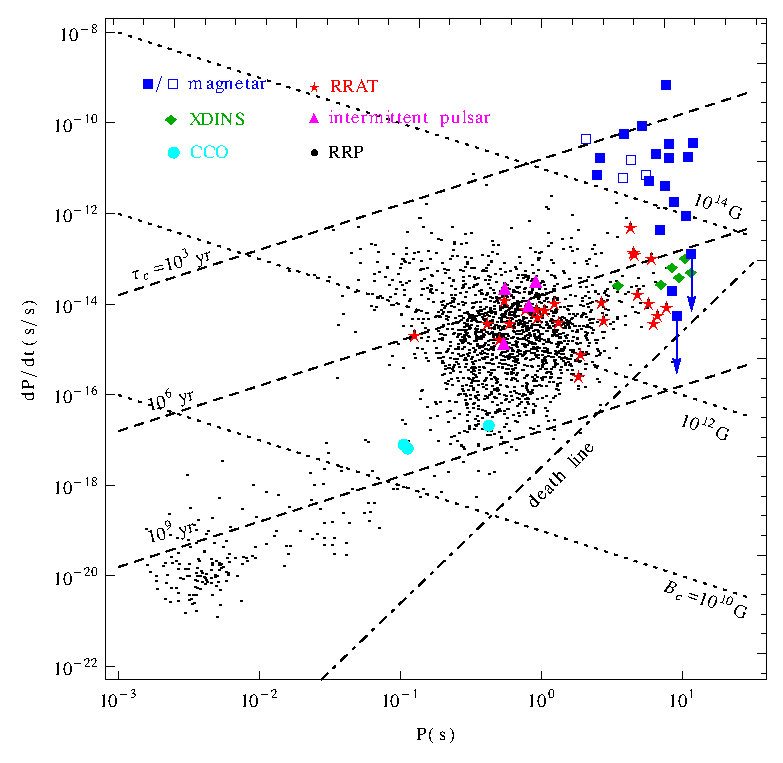
\includegraphics[scale=0.99]{PPdot_PSRLikeObjects.eps}
				\caption{\small\
				Распределение известных пульсаров на диаграмме период -- производная периода. Миллисекундные аккрецирующие пульсары кучкуются в левой нижней части диаграммы.  Линии равного магнитного поля --- пунктирные прямые с наклоном $-1$
				в силу зависимости \eqref{eq:BPPdot}.
				Рисунок взят из работы \cite{Tong2014}, диаграмма построена по данным каталога пульсаров ATNF \cite{ATNF}.
				}\label{fig:PPdot}
			\end{figure}
			Вращательная энергия в случае однородного вращения может быть записана через момент инерции звезды $I$ как $E = I\Omega^2 /2 $.
			Таким образом, измеряя период вращения звезды $P=2\pi/\Omega$ и его производную по времени $\dot{P}$, можно оценить величину магнитного поля на её поверхности из формулы \eqref{loss} так:
			\begin{equation}\label{eq:BPPdot}
				B^2=-\frac{I\dot{\Omega}}{A\Omega^3}=\frac{IP\dot{P}}{4\pi^2A}.
			\end{equation}
			Подставляя некоторые типичные параметры и характерные для нейтронных звезд величины, можно получить порядковую оценку на типичное магнитное поле миллисекундного пульсара \be
			B\sim  10^{8} \sqrt{ \frac{\dot{P}[\text{с/с}]}{10^{-20}} P[\text {мс}]} \text{ Гс},
			\ee 
			что является относительно большой величиной по сравнению с магнитными полями обычных звёзд и даже белых карликов. 
			Однако, среди всего многообразия различных видов пульсаров, миллисекундные имеют наиболее слабые магнитные поля (рис.~\ref{fig:PPdot}).  
			Таким образом, имеют самые малые значения дипольного магнитного поля среди всего многообразия различных типов пульсаров, так как кроме чрезвычайно малых периодов, миллисекундные пульсары, как правило, выделяются еще и невероятно малыми производными периода. 
			Так, для некоторых пульсаров производная периода может достигать $10^{-20}$ с/с, что делает миллисекундные пульсары  так же источниками самых стабильных периодических сигналов во  Вселенной.  


		% subsection subsection_name (end)

		\subsection{Структура и уравнения состояния} % (fold)
		\label{sub:EOS}
			На данный момент на Земле в лабораториях недостижимы такие условия, как
			очень сильное стационарное магнитное поле, колоссальное высокое давление и предельно высокая плотность вещества, 
			описанные в пункте~\ref{sub:NS}.
			Поэтому, к сожалению, вещество в таком состоянии не поддается экспериментальному изучению. 
			Чтобы изучать законы, по которым существует вещество в таких экстремальных условиях, остается только наблюдать за подобными явлениями в космосе.
			Ещё до первого наблюдательного обнаружения пульсаров, обсуждалась \cite{Oppenheimer1939} возможность путём изучения их свойств получать знания о характеристиках и параметрах вещества в экстремальных состояниях.
			Наблюдая за нейтронными звездами и моделируя различные сценарии процессов, которые могут протекать в их недрах, 
			современные ученые надеются продвинуться в изучении межнуклонного взаимодействия, квантовой хромодинамики и теории сверхтекучих жидкостей, в частности, нейтронного вещества.

			Нейтронную звезду окружает оптически тонкая атмосфера из высокоэнергитичных элементарных частиц. Под атмосферой располагается тонкий слой кулоновской жидкости. 
			Глубже, у нейтронных зведы выделяют кору, которая делится на внешнюю и внутреннюю, 
			а под ней располагается ядро, которое тоже делится на внешнее и внутреннее.
			Переходы между этими слоями плавные, но каждый из них обладает своими особыми свойствами.
			Внешняя кора состоит из атомных ядер железа, сложенных в кристаллическую решетку и вырожденных электронов. 
			Внутренняя кора состоит из тяжелых атомных ядер переобогощенных нейтронами и самих свободных нейтронов. 
			Эти ядра могут складываться в различные конфигурации, схожие с жидкими кристаллами. 
			При повышении плотности расстояние между ядрами сначала становится сравнимым с размерами самих ядер, а после и сами ядра начинают сливаться между собой.
			По мере возрастания давления различные конфигурации слившихся ядер и пустот между ними сменяют друг друга, пока на границе с ядром не превращаются в однородную ядерную материю. 
			Сами эти конфигурации получили называние ядерной пасты.
			Кора имеет толщину всего около 10\% радиуса нейтронной звезды.
			Считается, что ядро жидкое и состоит из вырожденных нейтронов с малой примесью вырожденных заряженных частиц --- протонов и электронов.
			Внутреннее ядро выделяется у массивных нейтронных звезд, плотность вещества в центре которых превышает ядерную более чем в два раза, а из чего может состоять такое плотное вещество в настоящее время точно не известно.
			В ядре и внутренней коре нейтронной звезды возможна сверхтекучесть нейтронного компонента, а также для протонного компонента при плотностях порядка ядерных возможна сверхпроводимость. 
			Эти эффекты имеют больше значение для физики нейтронных звезд, а их величины напрямую зависят от реализующегося уравнения состояния.  

			\begin{figure}[H]
				\centering
				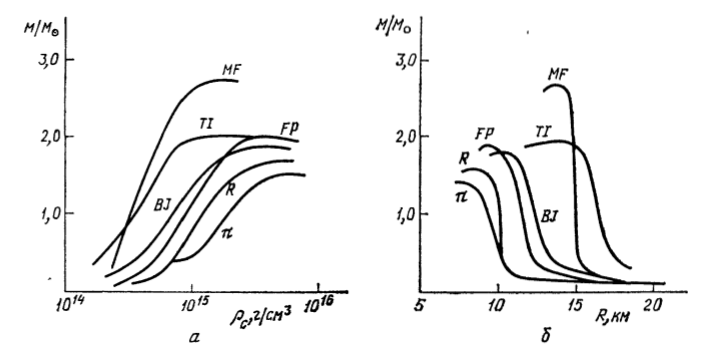
\includegraphics[scale=0.6]{B87EOS.png}
				\caption{\small
				Приведенные в обзоре \cite{Beskin1987} зависимости гравитационной массы нейтронной звезды $M$ от ее радиуса $R$  и центральной плотности $\rho_c$. 
				Определив с высокой точностью соотношения между массой и радиусом нейтронной звезды, становится возможным определить правильную модель состояния вещества в её недрах и условия там.}
				\label{B87EOS}
			\end{figure}

			\begin{figure}[H]
				\centering
				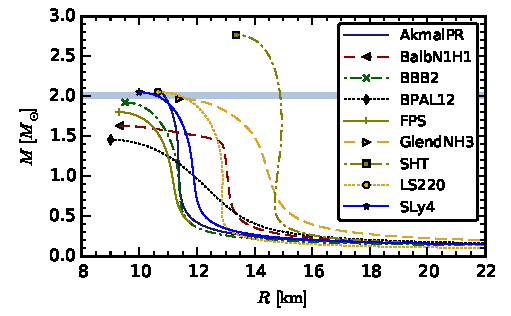
\includegraphics[scale=1.7]{Ch15EOS}
				\caption{\small
				Зависимости масса -- радиус для набора различных моделей уравнения состояния, использованных в исследовании \cite{Chirenti2015}.
				По сей день остается большое количество различных уравнений состояния, сильно противоречащих одна другой.}
				\label{Ch15EOS}
			\end{figure}


			

	\newpage

	\section{Мотивация}\label{Motivation}
		Большинство измерений радиусов нейтронных звёзд было получено путём моделирования тепловых спектров барстеров \cite{Miller2016}.
		Также, возможно получать ограничение на размеры нейтронной звезды путём исследования рентгеновских спектров остывающих молодых нейтронных звезд и транзиентных пульсаров в их спокойной фазе \cite{Heinke2013}.  

		Одним из альтернативных методов основан на исследовании профилей импульсов аккрецирующих пульсаров. 
		Большинство уравнений и алгоритмов этого метода были изначально выведены в \cite{Poutanen2003}. 
		Согласно этой модели, вблизи некоторой области поверхности нейтронной звезды имеется горячее пятно --- разогретая ударная волна около магнитного полюса звезды, где выделяется гравитационная энергия.
		Если ось магнитного диполя не совпадает с осью вращения, вещество из аккреционного диска падает на звезду так же не симметрично относительно оси вращения, а больше с той стороны, где в данный момент времени ближе диск. 
		Соответственно, в этом месте и образуется горячее пятно.
		Газ в горячем пятне вращается вокруг нейтронной звезды с частотой равной к частоте вращения самой звезды.
		Мягкое тепловое электромагнитное излучение нейтронной звезды комптонизуется в горячей плазме пятна с электронной температурой порядка 50 кэВ.
		Так же излучение претерпевает аберрацию и эффект Доплера,  создаваемый быстрым вращением звезды, и в дальнейшем распространяется в пространстве-времени искривленном гравитацией нейтронной звезды.  
		Таким образом, наблюдатель видит зависящую от энергии форму импульса, которая несет в себе информацию о параметрах нейтронной звезды:
		относительная скорость движения точки на поверхности содержит информацию о радиусе, а компактность звезды определяется отношением между массой и радиусом звезды. 
		Следовательно, из тщательного анализа форм импульсов можно получить эти параметры нейтронной звезды.

		Однако, к сожалению, неизвестных величин в этой модели оказывается слишком много для точного определения всех параметров нейтронной звезды \cite{Poutanen2008}, хотя в некоторых случаях позволяют получить хорошие результаты в виде ограничений на эти параметры \cite{Leahy2007}.
		На практике оказывается, что для получения параметров пульсара с достаточной точностью, он должен иметь частоту вращения в несколько сотен герц, так же плоскость его экватора и положение его пятна не должны иметь слишком большой угол с направлением на наблюдателя \cite{Miller2016}.
		В связи с быстрым вращением, нейтронная звезда принимает форму сплюснутого сфероида. 
		Влияние этого факта на кривые яркости изучалось в \cite{Cadeau2007} и позднее, например, в \cite{Leahy2006}. 

		Несмотря на несферичность нейтронной звезды, распространение света в непосредственной близости к звезде можно рассматривать в приближении Шварцшильдовской метрике \cite{Morsink2007}. 
		Так же предполагается, что излучение горячего пятна азимутально симметрично относительно локальной нормали, а форма звезды симметрично относительно оси вращения. 

		В скором будущем с запуском космических рентгеновских поляриметрических обсерваторий таких, как \begin{itemize}
			\item миссия XIPE, планируемая Европейским Космическим Агентством \cite{XIPE}, 
			\item спуник IXPE, который NASA планирует запустить в конце 2020 года; целями двухгодичной миссии являются изучение активных галактических ядер, микроквазаров и пульсаров \cite{IXPE},
			\item проект eXTP, готовящийся совместно Китайской Академией Наук и несколькими крупными университетами стран Европы к запуску в 2026 году 
			\cite{eXTP},
		\end{itemize}
		станет возможным получать информацию не только из кривых яркости, но и из колебания степени поляризации излучения и её позиционного угла.
		Это напрямую поможет измерять наклон оси вращения пульсара к лучу зрения и к магнитной оси. 
		Ожидается, что новые ограничения, получаемые из поляризационных наблюдений пульсаров, помогут значительно улучшить точность определения масс и радиусов этих объектов.
		Помимо этого можно будет узнать температуру мягкого излучения, которое комптонизуется в слое горячей плазмы, и температуру электронов в этой плазме. 
		Тем самым, возможно будет проверить основную модель образования спектров аккрецирующих миллисекундных пульсаров.

		В работе \cite{Viironen2004} для аккрецирующих миллисекундных пульсаров изучается и яркость рентгеновского излучения, и свойства его поляризации.
		Моделируется зависимость потока рентгеновского излучения, степени его поляризации и позиционного угла поляризации от фазы вращения нейтронной звезды.
		Рассматривается сферическая звезда с горячим пятном (или двумя диаметрально противоположно расположенными) на поверхности, которое излучает частично поляризованное излучение. 
		Ударная волна рассматривается как плоско-параллельный слой электронного газа, ширина которого много выше его вертикальной высоты. 
		Значения поляризации рассчитываются в приближении томсоновского рассеяния на частицах этого газа. 
		Спектр излучения и поляризацию в нем в этой работе предлагалось рассчитывать из соображения, что каждое последующее рассеяние фотона придает ему постоянный сдвиг по энергии, но точность этого приближения не обсуждалась.  

		%\textbf{Кто еще чем-то таким занимался занимался? И чем моя работа отличается от ихних?}
		
		Идея этой работы заключается  в том, чтобы разработать код, моделирующий совместно спектральный поток и поляризацию от пульсара в зависимости от фазы. 
		Эта задача логически разбивается на две независимые подзадачи. \begin{enumerate}
			\item Учесть приплюснутость нейтронной звезды в результате её быстрого вращения в методе расчета наблюдаемых поляризационных свойств излучения с элемента поверхности в зависимости от фазы звезды. 
			Эту задачу условно можно назвать внешней, так как предметом её рассмотрения является преобразование свойств света после излучения с поверхности нейтронной звезды и его распространение в искривленном гравитационным полем пульсара космическом пространстве. 
			\item Рассчитать спектральную интенсивность и поляризацию излучения в результате комптоновского рассеяния в оптически тонком однородном слое горячего электронного газа аккреционной ударной волны. В противопоставление предыдущей подзадаче, эту можно уловно назвать внутренней, так как её целью является моделирование комптонизации начального чернотельного излучения внутри оптически тонкого слоя горячей электронной плазмы.
		\end{enumerate}

		Результаты такого моделирования в будущем предполагается сравнить сравнить с результатами наблюдений будущих рентгеновских поляриметрических космических миссий.


	\newpage

	\section{Наблюдаемые поляризационные свойства излучения в зависимости от фазы звезды (внешняя задача)}\label{Outer}
		В этом разделе обсуждается преобразование параметров Стокса между поверхностью нейтронной звезды и приёмником космического аппарата. 
		Методы, изложенные в этом разделе, по большей части основаны на методах работ \cite{Viironen2004} и \cite{Poutanen2006}. 
		Описания основных геометрических эффектов из-за сплюснутости звезды  берут начало в статье\cite{Morsink2007}.  

		\subsection{Геометрия звезды}\label{sub:GG}
		    Рассматривается нейтронная звезда массы $M$, вращающаяся с частотой $\nu > 300$ Гц, при которой отличие формы звезды от сферической можно считать значительным \cite{Cadeau2007}. 
		    Ось вращения пульсара является осью его симметрии и осью аппликат $z$ в неподвижной системе отсчета. 
		    Направление оси $x$ выбирается так, чтобы направление на бесконечно удаленного наблюдателя $\bm{k}$ лежало в плоскости $xz$.
		    Вектор $\bm{k}$, указывающий на наблюдателя, составляет с осью вращения пульсара угол $i$. 

		    Пусть небольшое пятно располагается на полярном расстоянии (кошироте) $\theta$ от северного полюса вращения пульсара. 
		    Фаза пульсара $\varphi$ отсчитывается от плоскости $xz$, которую пересекает пятно в момент времени $t=0$, в сторону оси $y$, дополняющей базис до правой тройки векторов, и увеличивается со временем. 

			\begin{figure}[H]
				\centering
				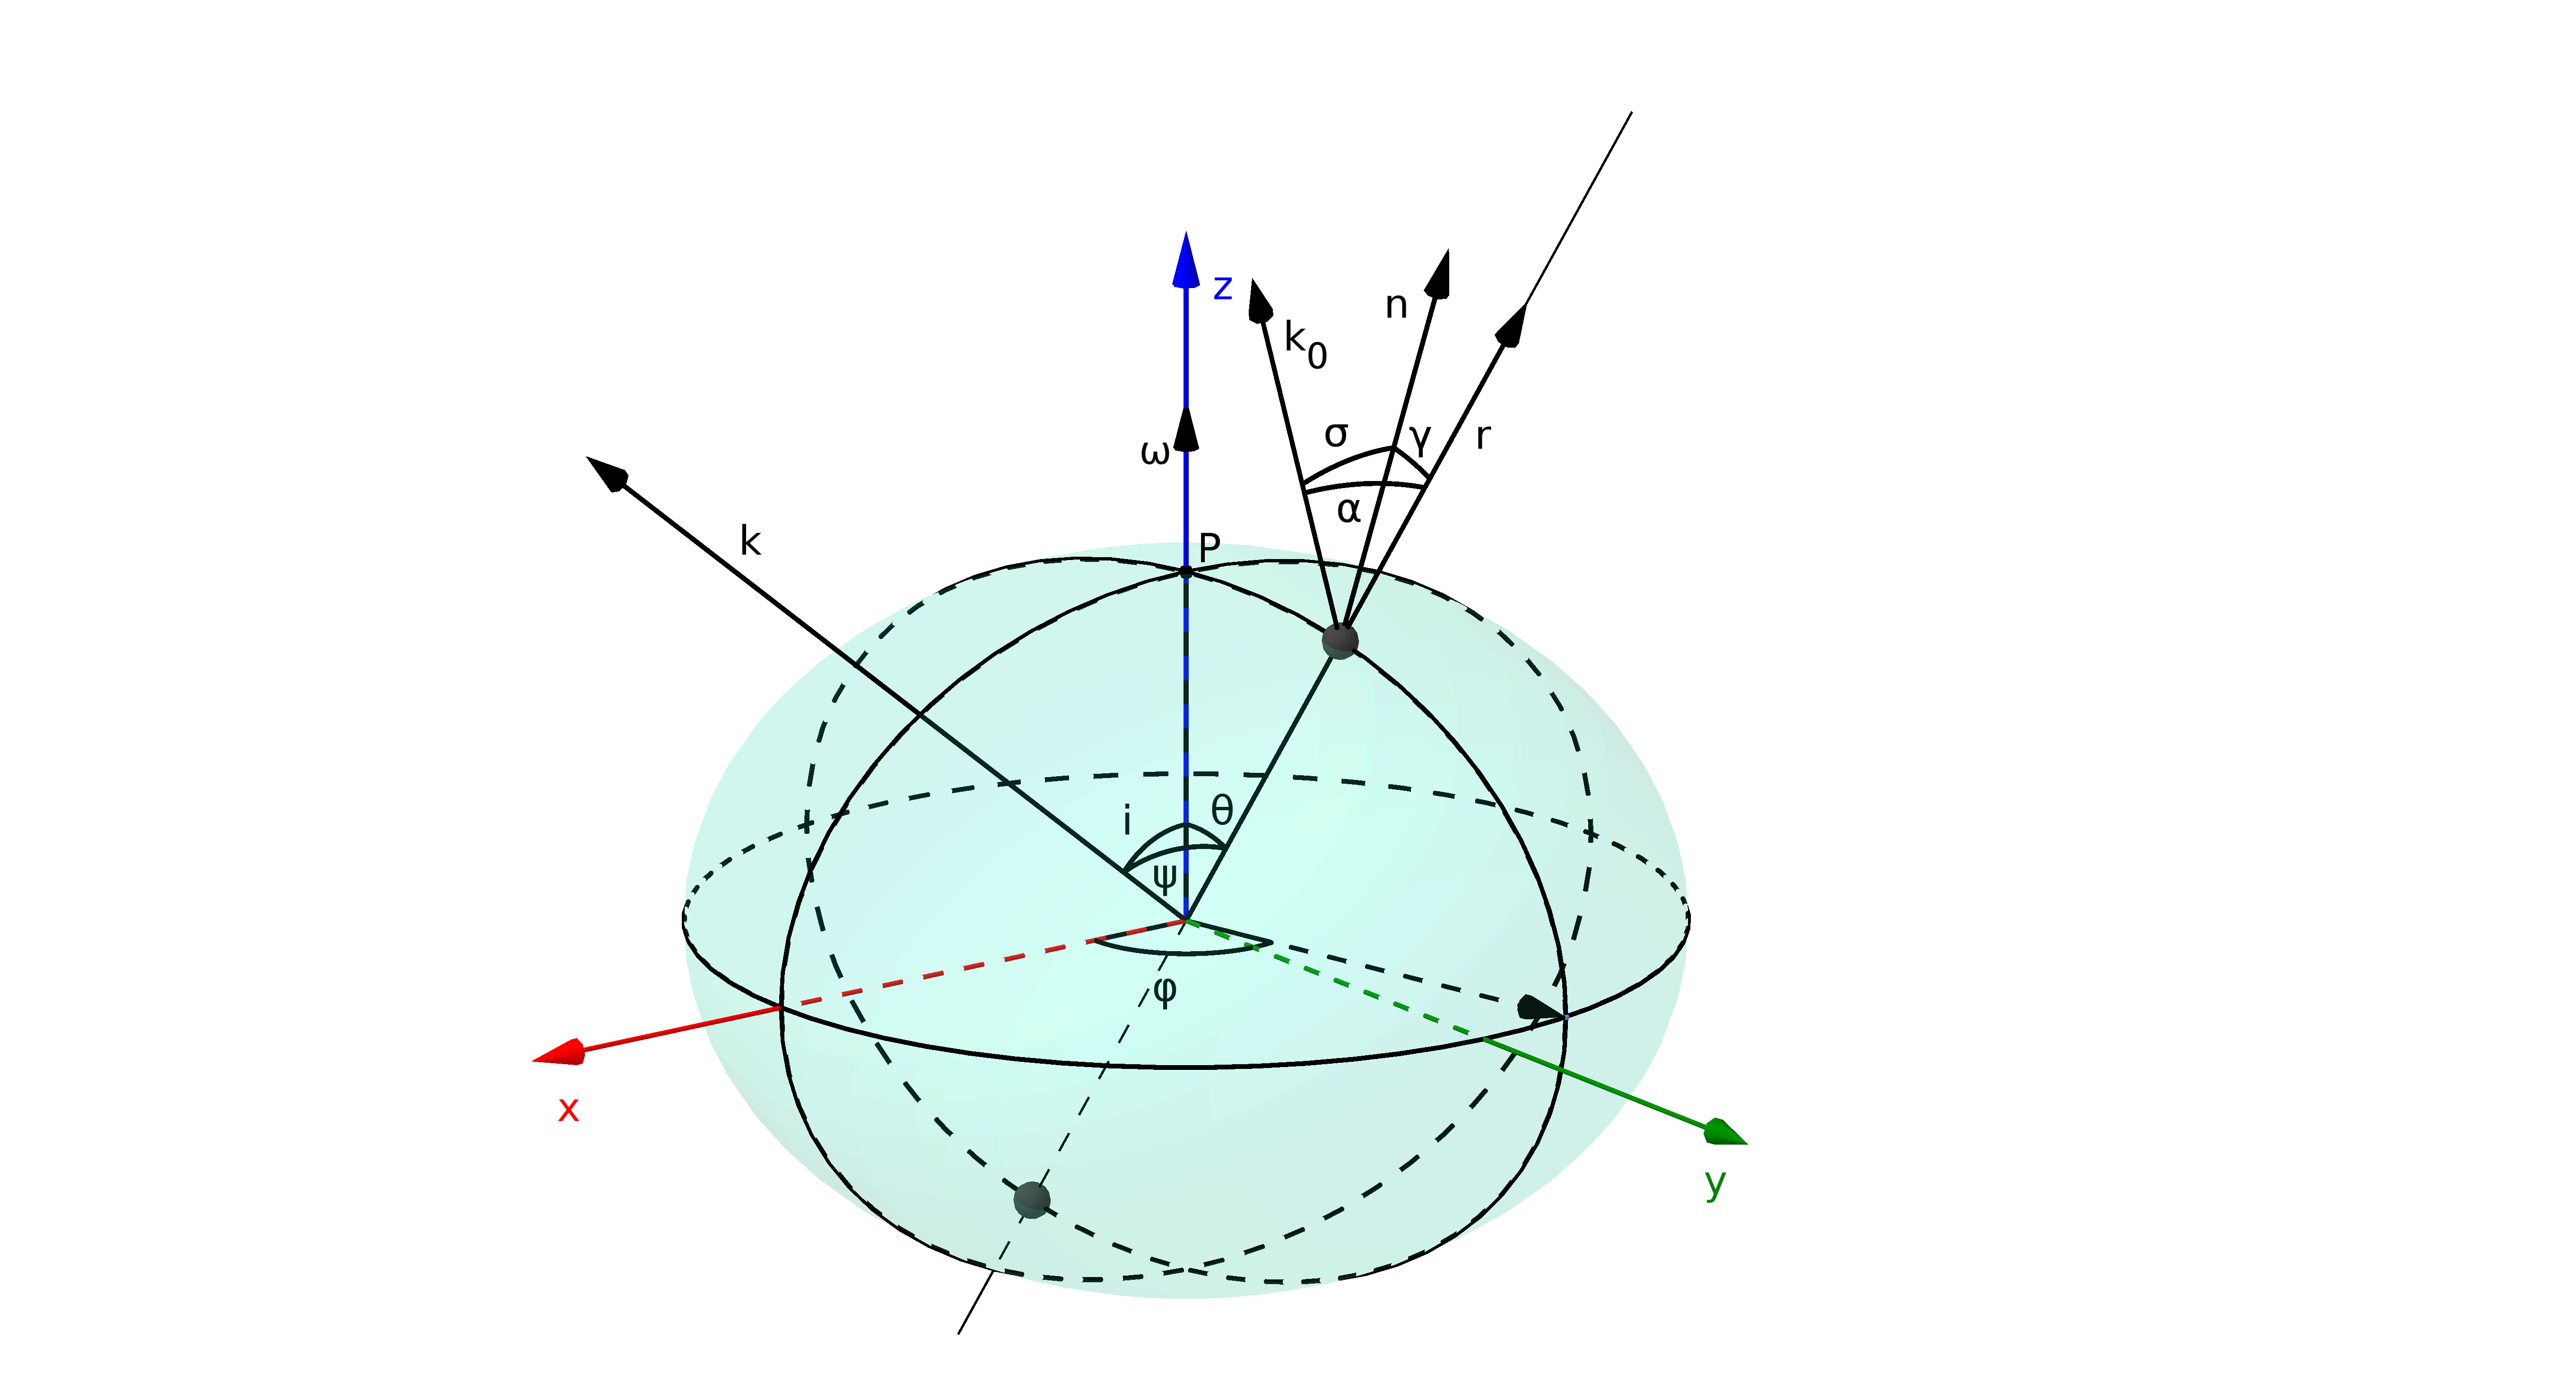
\includegraphics[scale=0.4]{fig1.png}
				\caption{\small
				Иллюстрация к геометрии задачи.}
				\label{geogebra0}
			\end{figure}

		    В каждый момент времени для пятна определены 3 единичных вектора: \begin{itemize}
		    	\item радиус-вектор $\bm{r}$, определяющий положение пятна на поверхности звезды относительно центра,
		    	\item вектор нормали $\bm{n}$ к поверхности пульсара,
		    	\item вектор $\bm{k_0}$, в направлении которого испущенное излучение в конечном счете достигнет наблюдателя.
		    \end{itemize}
		    Взаимное направление этих векторов определяется углами: 
		    \begin{itemize}
		    	\item $\gamma$ --- между $\bm{n}$ и $\bm{r}$,
		    	\item $\alpha$ --- между $\bm{r}$ и $\bm{k_0}$ и 
		    	\item $\sigma$ --- между $\bm{n}$ и $\bm{k_0}$.
		    \end{itemize}
		    Взаимное расположение всех перечисленных элементов показано на рисунке \ref{geogebra0}.
		    Например, вектор $\bm{r}$ в неподвижной системе отсчета запишется как 
		    \be 
		    \bm{r}=(\sin\theta\cos\varphi,\sin\theta\sin\varphi,\cos\theta),
		    \ee
		    а единичный вектор, указывающий на наблюдателя --- как
		    \be
		    	\bm{k}=(\sin i, 0 , \cos i),
		    \ee
		    а угол между ними, обозначенный как $\psi$, можно выразить так:
		    \be\label{cospsi}
		    	\cos \psi = \bm r \cdot \bm k = 
		    	 \cos i \cos\theta + \sin i \sin\theta\cos\varphi.
		    \ee

		    Форму звезды можно задать функцией 
		    	 шварцшильдовской координаты 
		    $R(\theta)$
		     точки поверхности на данном полярном расстоянии. 
		    Поскольку звезда вращается, пятно движется в лабораторной системе с безразмерной скоростью $\bm{\beta}=\bm{\hat\beta} \beta$, которая представляется в виде произведения единичного вектора движения 
		    \be\label{betahat}
		    	\bm{\hat\beta}=(-\sin\varphi,\cos\varphi,0)
		    \ee
		    и безразмерного (в единицах скорости света) модуля скорости 
		    \be
		    	\beta=\frac v c = \frac{2 \pi R(\theta) \sin\theta}{\sqrt{1-r_s/R(\theta)}} \frac{\nu}{c},
		    \ee
		    где гравитационное красное смещение имеет несколько вариантов обозначения
		    \be
		    	\left(1-\frac{r_s}{R(\theta)}\right)^{-\frac12}=\frac1{\sqrt{1-u}}=1+z.
		    \ee
		    Величина скорости равносильно задается соответствующим Лоренц-фактором
		    \be\label{Lorentz-factor}
		    	\Gamma=\frac1{\sqrt{1-\beta^2}}.
		    \ee

		    Угол $\gamma$ в силу осевой симметрии лежит в плоскости меридиана и зависит только от широты.
		    Тригонометрические функции этого угла можно представить в форме 
		    \be
		    \cos\gamma=\frac1{\sqrt{ 1+ f^2(\theta) }},
		    \ee
		    \be
		    \sin\gamma=\frac{f(\theta)}{\sqrt{ 1+ f^2(\theta) }},
		    \ee
		    где функция $f$ задается через функцию формы звезды и её производную
		    \be\label{eq:shape}
				f(\theta)= \frac{1+z(\theta)}R\frac{\df R}{\df \theta}.
			\ee

		    В этой работе используется одна из недавних моделей, приведенная в \cite{AlGendy2014}.
		    Согласно ей, пульсар имеет форму
		    \be
		    	R(\theta)=R_e\left(1+o_2(x,\bar\Omega)\cos^2(\theta)\right), 
		    \ee 
		    где коэффициент
		    \be
		    o_2(x,\bar\Omega)=\frac{R_p-R_e}{R_e}\approx\bar\Omega^2(1.030x-0.788)
		    \ee
		    определяет различие между экваториальным радиусом $R_e$ и полярным $R_p$ и зависит от 
		    безразмерного параметра компактности звезды
		    \be
		    x=\frac{GM}{c^2R_e}=\frac{r_s}{2R_e}
		    \ee
		    и безразмерной круговой частоты её вращения
		    \be
		    \bar\Omega=\Omega\left(\frac{R_e^3}{GM}\right)^{\frac12}.
		    \ee
		    Данное приближение дает форму звезды с процентной точностью для $\bar\Omega^2<0.1$. 
		    Для реалистичных уравнений состояния большинство нейтронных звезд с $\nu<700$ Гц и $M>M_{\odot}$ удовлетворяют этому условию. 

		\subsection{Форма пространства}\label{sub:SS}
		    Излучившийся с поверхности нейтронной звезды в направлении $\bm{k_0}$ в неподвижной системе отсчета фотон должен на бесконечно большом расстоянии от звезды иметь направление распространения вдоль вектора  $\bm{k}$,
		    отличающегося от $\bm{k_0}$ из-за искривления световых траекторий сильным гравитационным полем звезды.
		    Так как свет в метрике Шварцшильда распространяется по плоским траекториям, вектор $\bm{k}$ должен лежать в плоскости, составленной векторами $\bm{k_0}$ и $\bm r$. Сечение этой плоскостью изображено на рисунке~\ref{fig:trajectory}.
		    Иначе говоря, вектор 
		    \be\label{k0}
		    	\bm{k_0}=\frac{\sin\alpha \bm k + \sin(\psi-\alpha) \bm r}{\sin \psi}
		    \ee 
		    лежит между векторами $\bm{k}$ и $\bm{r}$.  


		    Точное соотношение между углами $\alpha$ и $\psi$ в Шварцшильдовской метрике записывается (см. <<Гравитация>> \cite{Misner1973} ) в виде интеграла
		    \be\label{eq:bendexact}
		    	\psi(R,\alpha)=\int_R^{\infty} \frac{\df r}{r^2} \left(\frac1{b^2}-\frac1{r^2}\left(1-\frac{r_s}r\right)\right)^{-\frac12},
		    \ee
		    с прицельным параметром 
		    \be\label{eq:impact}
		    	b=R(1+z)\sin\alpha.
		    \ee
			\begin{figure}[H]
				\centering
				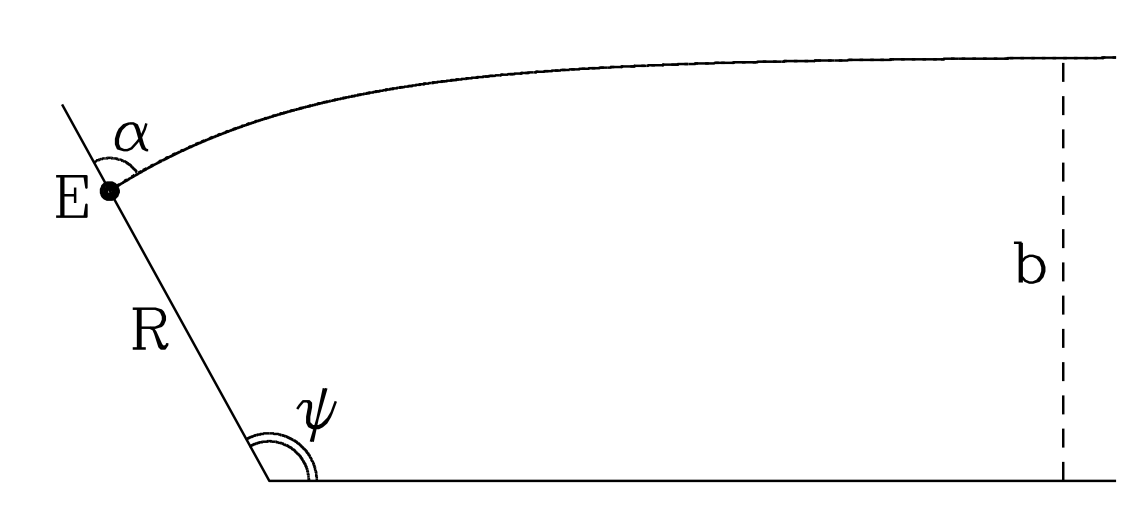
\includegraphics[scale=0.3]{Bb02.png}
				\caption{\small
				Иллюстрация возможной траектории фотона \cite{Beloborodov2002}.}\label{fig:trajectory}
			\end{figure}
		    		
		    Поскольку звезда имеет сплюснутую форму, теоретически угол 
		    $\alpha$
		    может быть даже больше чем 
		    $\frac{\pi}2$.
		    В таком случае зависимость 
		    $\psi(\alpha)$
		    принимает форму 
		    \be
		    	\psi(R,\alpha)=2\psi_{max}-\psi(R,\pi-\alpha)
		    \ee
		    где угол
 			$\psi_{max} = \psi (p,\pi-\alpha)$
		   	рассчитывается на перицентрическом расстоянии 
		    $p$, которое удовлетворяет уравнению
		    \be
				b=\frac{p}{\sqrt{1-r_s/p}},
			\ee
			решение которого можно записать следующим образом
			\be
				p=-\frac{2b}{\sqrt3}\cos \left(\frac13 \arccos \left(\frac{3\sqrt3 r_s}{2b}\right)+\frac{2\pi k}{3}\right).
			\ee
			

		    Для данной фазы пульсара $\varphi$ излучение с разных точек его поверхности будет доходить до наблюдателя в разные моменты времени \be\label{eq:timedelay}
		    \varphi_{obs} = 
		    \varphi+\Delta\varphi(b,R)\ee
		    из-за разности длин световых траекторий.  
		    Световая задержка зависит от прицельного параметра $b$ и расстояния до центра звезды $R$, на котором был излучен фотон. 
		    При одинаковом 	$R$ задержка по времени $\Delta t(b)$  фотона, имеющего прицельный параметр $b$, относительно фотона с нулевым прицельным параметром (и следовательно нулевым углом $\alpha$) выражается \cite{Pechenick1983} через интеграл 
		    \be\label{eq:timelag}
		    	c\Delta t_R(b) = \int_R^{\infty} \frac{\df r}{1-r_s/r}\left(\frac{r}{\sqrt{r^2-b^2(1-r_s/r)}}-1\right).
		    \ee 
		    Но надо еще учесть сплюснутость звезды, то есть то, что излучение приходит с разных $R$. 
		    Задержка между двумя фотонами излученными с нулевым прицельным параметром с расстояния $R$ и некоторого заранее заданного и превышающего $r_s$, к примеру $R_e$, вычисляется через 
		    \be
		    	c\Delta t(R) = \int_R^{R_e} \frac{\df r }{1-r_s/r} = R_e-R+r_s \ln\left(\frac{R_e-r_s}{R-r_s}\right).
			\ee 
			Смещение фазы будет пропорционально сумме этих величин
			\be
				\Delta\varphi(\varphi)= 2\pi\nu(\Delta t_R(b(\varphi)) +\Delta t(R)).
			\ee
			Для любого малого пятна на поверхности пульсара, мы можем  фазу пульсара $\varphi$ однозначно сопоставить
			\be2 \pi t=P\varphi_{obs}\ee
			времени, когда поток фотонов испущенных в этой фазе достигнет приемника.    
		    Способ численного расчета интегралов \eqref{eq:timelag} и \eqref{eq:bendexact} описан в приложении \ref{app:exact}.

		    Интенсивность и поляризация излучения пятна задаётся в системе отсчета, где это пятно покоится. 
		    В этой системе отсчета излучение исходящее от поверхности в направлении 
		    $\bm{k}_0'$
		    под углом 
		    $\sigma'$
		    к вертикали подвергается эффекту релятивистской аберрации. 
		    Косинус этого угла 
		    \be\label{eq:cossigmaprime}
		    	\mu=\cos \sigma'=\delta\cos\sigma
		    \ee
		    при переходе в лабораторную систему домножается \cite{Poutanen2003} на Доплер-фактор
		    \be\label{Doppler-factor}
		    	\delta=\frac1{\Gamma(1-\bm{k_0}\cdot\bm{\beta})},
		    \ee
		    где скалярное произведение с использованием \eqref{k0} выражается через комбинацию углов
		  	\be\label{cosxi}
		  		\bm{k_0}\cdot\bm{\beta}=\frac{\sin \alpha }{\sin\psi} \bm{k}\cdot\bm{\hat\beta} \beta=
		  		- \beta \frac{\sin \alpha }{\sin\psi} \sin i \sin \phi,
		  	\ee
		  	А сам $\cos \sigma$ может быть получен путём двухкратного применения сферической теоремы косинусов 
		  	ко всем обозначенным на рисунке~\ref{geogebra0} углам 
		  	и, затем, формулы \eqref{cospsi}:
			$$
		  		\cos\sigma=\cos \alpha \cos \gamma + 
		  		\frac{\sin\gamma}{\sin\theta}
		  		\frac{\sin\alpha}{\sin\psi}
		  		(\cos i - \cos\theta \cos\psi) =
		  	$$\be\label{eq:cossigma}
		  		=\cos \alpha \cos \gamma + 
		  		\frac{\sin\alpha}{\sin\psi}
		  		(\cos i \sin\theta - \sin i \cos\theta \cos\phi).
		  	\ee
			При малых углах $\psi$ в формулах
		  	\ref{eq:cossigma}
			и
		  	\ref{cosxi}
			во избежание деления двух малых величин друг на друга можно применить приближение Белобородова, показанное в  \cite{Beloborodov2002}
			\be\label{eq:beloborodovsapproximation}
				\cos\alpha\approx u + \cos\psi (1-u),
			\ee 
			которое иначе переписывается как
			\be
				\frac{1-\cos\alpha}{1-\cos\psi}\approx  1-u.
			\ee
			Отсюда имеем, что часто встречающееся в формулах
			отношение синусов
			\be\label{sinalphaoversinpsi}
				\frac{\sin\alpha}{\sin\psi} \underset{\psi \to 0}{\rightarrow} \sqrt{1-u}.
			\ee
			имеет предел, значение которого можно подставлять вместо этого отношения в случаях, когда пятно по отношению к наблюдателю располагается  
			почти плашмя.


		\subsection{Поток излучения}\label{sub:EF}
			Комбинация эффекта Доплера и гравитационного красного смещения дает соотношение \cite{Misner1973} между наблюдаемой интенсивностью на бесконечности и испускаемой интенсивностью в движущейся вместе с пятном системе отсчета в виде 
			\be\label{eq:shifts}
				I_x(\sigma)=\left(\frac{x}{x'}\right)^3 I'_{x'}(\sigma'),
			\ee
			где энергия сдвигается на величину
			\be
				\frac{x}{x'}=\delta\sqrt{1-u}.
			\ee

			Чтобы вычислить поток излучения, создаваемый этой интенсивностью, и фиксируемый наблюдателем в каждый момент времени, нужно знать телесный угол $\df \Omega$, который каждый излучающий участок поверхности занимает на небесной сфере. 
			Поскольку свет распространяется по шварцшильдовским геодезическим, этот телесный угол можно выразить \cite{Pechenick1983}
			в виде 
			\be\label{eq:dOmega}
				\df \Omega=\frac{b \df b \df \phi_o}{D^2},
			\ee
			где $D$ --- это расстояние от наблюдателя до звезды, а $\phi_o$ --- это азимутальный угол вокруг луча зрения $\bm k$.
			Прицельный параметр $b$ для фиксированной точки на поверхности с конкретным радиусом $R(\theta)$ является функцией только $\psi$. 
			Системы угловых координат $\{\psi,\phi_o\}$ и $\{\theta, \varphi \}$ связаны между собой соотношением
			\be
				\sin\psi \df\psi\df\phi_o=\sin\theta\df\theta\df\varphi.
			\ee
			Формула \eqref{eq:dOmega} с использованием \eqref{eq:impact}, \eqref{eq:shape} и \eqref{eq:cossigma} упрощается
			\cite{Poutanen2003,Morsink2007} 
			до вида
			\be\label{eq:solid}
				\df \Omega=\frac{\df S\cos\sigma}{D^2}\frac1{1-u}\pdv{\cos\alpha}{\cos\psi},
			\ee
			где значение частной производной определяется из интегрального определения  
			\eqref{eq:bendexact} функции $\psi(R,\alpha)$
			\be\label{eq:partial}
				\pdv{\cos\alpha}{\cos\psi}=\frac{\sin\alpha}{\sin\psi}\left(\pdv{\psi}{\alpha}\right)^{-1}.
			\ee
			В приближении \eqref{eq:beloborodovsapproximation} 
			формула \eqref{eq:solid}
			принимает привычный вид 
			\be
				\df \Omega=\frac{\df S\cos\sigma}{D^2}.
			\ee

			Бесконечно малый элемент площади, измеренный во вращающейся со звездой системе отсчета может быть сосчитан  с учетом несферичности поверхности звезды 
			\cite{Morsink2007} по формуле 
			\be
				\df S'(\theta)=\Gamma R^2(\theta)\frac{\sin\theta}{\cos\gamma}\df \theta \df \varphi.
			\ee

			Так как проекция площади потока излучения на плоскость перпендикулярную направлению его распространения является лоренцевским инвариантом 
			\cite{Lightman1975}, наблюдаемая площадь малого элемента пятна в лабораторной системе отсчета и связь между углами $\sigma$ и $\sigma'$ описывается соотношением 
			\be	
				\df S\cos\sigma=\df S'\cos\sigma',
			\ee
			что, согласно \eqref{eq:cossigmaprime}, можно эквивалентно записать как
			\be
				\df S = \delta \df S'.
			\ee


			Для простоты переобозначим исходящую спектральную интенсивность $I'_{x'}(\sigma')$ в системе отсчета пятна в $I'(x',\mu)$, переходя от угла к его косинусу. Тогда, используя \eqref{eq:solid} и \eqref{eq:shifts}, можно записать формулу для потока приходящего излучения от элемента площади пятна   
			\be\label{eq:flux}
				\df F_x=I_x \df \Omega= \delta^3\sqrt{1-u} \frac{\df \cos\alpha}{\df \cos\psi}  \frac{ \df S'\mu}{D^2} I'(x',\mu). 
			\ee
			В последней формуле под $I'$ может пониматься не только непосредственно интенсивность излучения, но, в том числе, и другие параметры Стокса.

		\subsection{Степень поляризации и позиционный угол}\label{sub:LB}
		
			Поляриметр наблюдает поляризацию излучения пульсара в картинной плоскости неба в неподвижной системе, в то время как данные получаемые из моделирования поляризационных спектров излучения вычисляются в системе неподвижной звезды.  
			Для того, чтобы привести излучение звезды в каждый момент времени к некой единой системе, нужно выполнить несколько последовательных шагов по переводу поляризационного вектора (вектора, составленного из параметров Стокса) между различными поляризационными базисами.
			Для начала введем главный поляризационный базис
			\be 
				\label{mbasis}
				\bm{e}_1^m = \frac{\bm{z}-\cos{i} \bm{k}}{\sin{i}},\qquad 
				\bm{e}_2^m = \frac{\bm{k} \times \bm{z}}{\sin{i}}.
			\ee
			Вектор $\bm{e_1^m}$ сонаправлен проекции оси вращения пульсара на картинную плоскость, а вектор $\bm{e_2^m}$ перпендикулярен ему.
			Этот базис зафиксирован в лабораторной системе отсчета, поскольку ось вращения пульсара (вдоль $\bm{\omega}$ или $\bm{z}$) крайне стабильна, и луч зрения (вдоль $\bm{k}$) так же не меняется со временем.
			Вектор поляризации для наблюдателя лежит в этом базисе.

			Далее рассмотрим базис образованный радиус-вектором пятна $\bm{r}$ и вектором наблюдателя $\bm{k}$
			\be\label{rbasis}
			\bm{e}^r_1 = \frac{\bm{r}-\cos{\psi} \bm{k}}{\sin{\psi}},\qquad 
			\bm{e}^r_2 = \frac{\bm{k} \times \bm{r}}{\sin{\psi}}.
			\ee
			Этот базис описывает ту же плоскость, что и главный, но он вращается относительно него со временем.   
			Разница между позиционными углами поляризации в этих двух базисах обозначим $ \chi_0 $.
			Этот угол отсчитывается от компонента главного базиса $\bm{e}_1^m$ в сторону вектора $\bm{e}_1^r$ против часовой стрелки.
			Он равен углу между соответствующими ортами этих базисов. 
			Используя \eqref{cospsi}, его можно выразить для каждой фазы пульсара следующими формулами
			\be
			\cos{\chi_0}=\bm{e}_1^m \cdot \bm{e}^r_1 = \frac{\sin{i}\cos{\theta}-\sin{\theta}\cos{i}\cos{\varphi}}{\sin{\psi}} , 
			\ee \be 
			\sin{\chi_0}= - \bm{e}_1^m \cdot \bm{e}^r_2 = \bm{e}_2^m \cdot \bm{e}^r_1 = - \frac{\sin{\theta}\sin{\varphi}}{\sin{\psi}} ,
			\ee
			По значениям обеих тригонометрических функций угол $\chi_0$ может быть однозначно определен.
			Для сферической медленно вращающейся звезды этого преобразования уже достаточно. 
			Для того чтобы учесть кривизну поверхности звезды, рассмотрим базис образованный радиус-вектором $\bm{r}$ и вектором распространения света $\bm{k_0}$ вблизи поверхности звезды
			\be\label{basis}
			\bm{e}_1 = \frac{\bm{r}-\cos{\alpha} \bm{k_0}}{\sin{\alpha}},\qquad 
			\bm{e}_2 = \frac{\bm{k_0} \times \bm{r}}{\sin{\alpha}}=\bm{e}^r_2.
			\ee
			В связи с плоскостью световых траекторий степень и угол поляризации в этом базисе будет совпадать с соответствующими значениями в базисе \eqref{rbasis}
			\textbf{(Вроде правда)}, а вектора $\bm{e}_2$ и $\bm{e}^r_2$ равны между собой.
			Затем рассмотрим базис связанный с нормалью к поверхности пятна $\bm n $
			\be\label{nbasis}
			\bm{e}_1^n = \frac{\bm{n}-\cos{\sigma} \bm{k_0}}{\sin{\sigma}},\qquad 
			\bm{e}_2^n = \frac{\bm{k_0} \times \bm{n}}{\sin{\sigma}} .
			\ee
			Эти базисы лежат в одной плоскости и повернуты друг относительно друга на угол $\chi_1$.
			Этот угол аналогично вычисляется
			\be
			\cos{\chi_1}=\bm{e}_1^n \cdot \bm{e}_1 = \frac{\cos\gamma-\cos\alpha\cos\sigma}{\sin{\alpha}\sin\sigma} , 
			\ee $$ 
			\sin{\chi_1}= \bm{e}_2 \cdot \bm{e}^n_1 = \frac{\bm{n} \cdot (\bm{k_0}\times\bm{r} )}{\sin\alpha\sin\sigma}
			= \frac{\bm{k_0} \cdot (\bm{r}\times\bm{n} )}{\sin\alpha\sin\sigma}=
			$$\be
			= \frac{\sin\alpha}{\sin\psi} \frac{ \bm{k} \cdot (\bm{r}\times\bm{n} )}{\sin\alpha\sin\sigma}
			= \frac{ \sin\gamma\sin i \sin\varphi}{\sin\psi\sin\sigma}.
			\ee
			Этот базис связан с исходящим излучением вблизи пятна в неподвижной системе отсчета. 
			Чтобы учесть вращение плоскости поляризации в связи с релятивистским вращением поверхности, рассмотрим базис в системе отсчета покоящегося пятна
			\be\label{primebasis}
				\bm{e}_1' = \frac{\bm{n}-\cos{\sigma'} \bm{k_0'}}{\sin{\sigma'}},\qquad 
				\bm{e}_2' = \frac{\bm{k_0'} \times \bm{n}}{\sin{\sigma'}} .
			\ee
			Перепишем первый вектор
			в виде (см. \cite{Nagirner1993} ) 
			\be
			\bm{e}_1' = \frac{\bm{n}+
			\Gamma
			\delta
			\cos{\sigma} (\bm{\beta-k_0})}{\sqrt{1-\delta^2 \cos^2{\sigma} } }.
			\ee
			Угол релятивистского поворота обозначим $\chi'$.
			Используя обозначения \eqref{eq:cossigmaprime}  и \eqref{betahat},
			этот угол можно выразить формулой
			\be\label{sinchi}
			\sin{\chi'}=\bm{e}_1'\cdot \bm{e}_2^n =
			 \frac{\mu\Gamma\beta }{\sin{\sigma}\sqrt{1-\mu^2} } \bm{\hat\beta} \cdot(\bm{k_0} \times \bm{n}).
			\ee
			Тройное векторное произведение $\bm{\hat\beta} \cdot(\bm{k_0} \times \bm{n}) $, содержащееся в \eqref{sinchi}, можно преобразовать 
			\be\label{tripleproductoblate}
			 \bm{k_0} \cdot (\bm{n}\times\bm{\hat\beta} )=
			 \bm{k_0} \cdot \left(\bm{n} \times \frac{\bm{n} \times \bm{r}}{\sin{\gamma}}\right)=
			 \bm{k_0} \cdot \frac{\cos{\gamma}\bm{n} - \bm{r}}{\sin{\gamma}} =
			 \frac{\cos{\sigma}\cos{\gamma}-\cos{\alpha}}{\sin{\gamma}}.
			\ee
			И в конце концов получаем 
			\be\label{eq:chiprime}
			\sin{\chi'}=\bm{e}_1'\cdot \bm{e}_2^n =
			 \frac{\mu\Gamma\beta (\cos{\sigma}\cos{\gamma}-\cos{\alpha})}{\sin{\gamma}\sin{\sigma}\sqrt{1-\mu^2} }.
			\ee

			Стоит отметить, что несферичность звезды упрощает внешний вид вывода \eqref{tripleproductoblate}. 
			Если же звезда сферичная, то этой формулой воспользоваться уже не удастся, так как в знаменателе будет стоять синус нулевого угла $\gamma$ между нормальным и радиальным направлениями. 
			Чтобы получить формулу, не содержащую этого синуса в знаменателе, 
			рассмотрим касательный к меридиану вектор 
			\be
				\bm m = (- \cos \lambda \cos \phi, -\cos \lambda \sin \phi, \sin \lambda ),
			\ee
			где $\lambda=\theta-\gamma$ --- это угол между нормалью и осью вращения.
			И пусть $\zeta$ --- это угол, который этот вектор составляет с вектором $\bm k$ \be
			\cos\zeta=\bm m \cdot \bm k =  \cos i \sin \lambda - \sin i \cos \lambda \cos \phi .
			\ee 
			Тогда \eqref{tripleproductoblate} можно переписать в более универсальном виде
			$$
			 \bm{k_0} \cdot (\bm{n}\times\bm{\hat\beta} )=
			 \bm{k_0} \cdot \bm{m}=\frac{
			 \cos\zeta
			 \sin \alpha
			 - 
			 \sin\gamma 
			 \sin(\psi-\alpha)
			 }{\sin\psi}
			 =	
			$$\be\label{tripleproductpherical}
				=(\cos\zeta+\cos\psi \sin\gamma)\frac{\sin\alpha}{\sin\psi} - \cos \alpha\sin\gamma, 
			\ee
			где малость или даже равенство нулю угла $\gamma$ не создает вычислительных проблем, а при малых углах
			$\psi$
			для отношения синусов по прежнему можно использовать формулу \eqref{sinalphaoversinpsi}.

			В частности, для абсолютно сферической звезды 
			формулу \eqref{eq:chiprime},
			используя выражение \eqref{tripleproductpherical} для тройного произведения,
			можно переписать в виде
			\be\label{chiprimespherical}
			\sin{\chi'}=\bm{e}_1'\cdot \bm{e}_2^n =
			 \frac{\mu\Gamma\beta (\cos i \sin \theta - \sin i \cos \theta \cos \phi)}{\sin{\psi}\sqrt{1-\mu^2} }.
			\ee
			Косинус же этого угла можно выразить следующим способом    
			$$
				\cos\chi'=\bm{e}_1'\cdot \bm{e}_1^n =\frac{\bm n + \delta  \Gamma \cos\sigma (\bm \beta - \bm{k_0} ) }{\sqrt{1-\mu^2} }\cdot
				\frac{\bm n - \cos \sigma  \bm{k_0} }{\sin{\sigma}} = $$
			$$
				=\frac{1-\cos^2\sigma-\delta \Gamma \cos^2 \sigma \bm \beta \cdot \bm{k_0} }{\sin{\sigma}\sqrt{1-\mu^2} } 
				=\frac{\sin^2\sigma-  \cos^2 \sigma \bm \beta \cdot \bm{k_0} /(1-\bm \beta \cdot \bm{k_0}) }{\sin{\sigma}\sqrt{1-\mu^2} } =
			$$
			$$
				=\frac{\sin^2\sigma -\bm \beta \cdot \bm{k_0} \sin^2\sigma - \cos^2 \sigma \bm \beta \cdot \bm{k_0} }{\sin{\sigma}\sqrt{1-\mu^2} (1-\bm \beta \cdot \bm{k_0}) } 
				=\frac{\sin^2\sigma -\bm \beta \cdot \bm{k_0}  }{\sin{\sigma}\sqrt{1-\mu^2} (1-\bm \beta \cdot \bm{k_0}) } =
			$$\be\label{eq:coschiprime}
				=\frac{\sin^2\sigma + \beta \frac{\sin \alpha }{\sin\psi} \sin i \sin \phi }{\sin{\sigma}\sqrt{1-\mu^2} (1+ \beta \frac{\sin \alpha }{\sin\psi} \sin i \sin \phi) }.	
			\ee

			Комбинируя \eqref{eq:chiprime}, \eqref{tripleproductpherical} и \eqref{eq:coschiprime}, в итоге имеем выражение для тангенса
			\be
			\tg\chi' = \beta \cos \sigma \frac{
				\cos\zeta + \sin \gamma (\cos \psi - \frac
					{\sin \psi}
					{\sin \alpha}
				\cos \alpha)}
				{\frac{\sin \psi}{\sin \alpha}\sin^{2}\sigma + \beta \sin i \sin \phi}.
			\ee
			В случае сферической звезды оно совпадает с результатом, представленным в \cite{Viironen2004} и выглядит так
			\be
			\tg\chi' = \beta \cos \alpha \frac{\cos i \sin \theta - \sin i \cos \theta \cos \phi}{\sin \psi\sin\alpha + \beta \sin i \sin \phi}.
			\ee





			Ввиду симметрии, в системе отсчета покоящейся звезды излучение пятна не имеет круговой поляризации, а линейная поляризация описывается только одним параметром Стокса, то есть вектор поляризации коллинеарен одному из векторов базиса \eqref{primebasis}. 
			Круговая поляризация излучения в любой системе отсчета будет оставаться нулевой, поэтому будем рассматривать вектор Стокса содержащий только три компоненты $(F_I,F_Q,F_U)$.
			В базисе покоящегося пятна равен нулю так же позиционный угол поляризации, то есть и третий компонент вектора Стокса будет нулевым.
			Степень поляризации $P$ в этом случае определяется простым соотношением $F_Q=P F_I$.
			С вращением поляризационного базиса степень поляризации меняться не будет.
			В конечном счете, в главном базисе вектор Стокса примет форму 
			\be
				(F_I, F_Q \cos{2\chi},F_Q \sin{2\chi}),
			\ee
		    где позиционный угол поляризации
			\be
			\chi=\chi_0+\chi_1+ \chi'\ee
			получается путем сложения углов между промежуточными базисами.

			В случае, если помимо основного пятна рассматривается пятно, сформированное вокруг противоположного магнитного полюса нейтронной звезды, и если пятна имеют существенный размер и требуется считать потоки от малых элементов их площади $dS'$ по формуле \eqref{eq:flux}, то полный вектор Стокса получается путем простого суммирования параметров Стокса для всех элементов $m$ площади и каждого пятна 
			$$
				F_I^{tot}=\sum_m F_I^m, $$ \be
				F_Q^{tot}=\sum_m F_Q^m,\ee $$
				F_U^{tot}=\sum_m F_U^m. $$ 
			Тогда полная степень поляризации будет вычисляться как 
			\be\label{eq:Ptot}
				P^{tot}=\frac{\sqrt{(F_Q^{tot})^2+(F_U^{tot})^2}}{F_I^{tot}}, \ee
			а полный поляризационный угол, очевидно, через соотношение 
			\be\label{eq:chitot}
				\tg{2\chi^{tot}}=\frac{F_U^{tot}}{F_Q^{tot}}.
			\ee


		\subsection{Профили импульса}\label{sub:LC}
			Используя вышеописанный метод, уже можно моделировать профили импульсов для разных параметров пульсара. 
			Рассматриваются два диаметрально противоположных друг другу пятна точечного размера.   
			На данном этапе можно рассмотреть случай рентгеновской вспышки, описаный в \cite{Viironen2004}.
			Рассматривается плоско-параллельная осесимметричная полубесконечная атмосфера с Томсоновским законом рассеяния.
			В итоге рассматривается интенсивность $I_x$ с чернотельным спектром, заданным температурой \be\label{eq:Theta}
			\Theta_{bb}=\frac{kT_{bb}}{m_ec^2}=0.002\ee
			с зависимостью от косинуса зенитного угла $\mu$ в виде
			\be
			I_x(\mu)=(1 + 2.06\mu)I_x.\ee
			Степень поляризации излучения принимает вид \be
				P=-\frac{1-\mu}{1+3.582\mu}11.71\%,
			\ee
			то есть основное направление колебаний вектора напряженности электрического поля происходит вдоль $\bm{k_0} \times \bm n$.
			Степень поляризации закономерно приближается к нулю вблизи вертикальных направлений ввиду осевой симметрии.
			Данное приближение здесь используется только для демонстрации величин различных поправок, рассматриваемых в этом разделе.
			Моделированию спектров и параметров поляризации для рентгеновского пульсара посвящен раздел \ref{Spectra}.

			Рассмотрим типичную нейтронную звезду с параметрами $M=1.4M_{\odot}$ и $R_e=12$ км, но с большой частотой вращения $\nu=600$ Гц. При этом сплюснутость звезды оказывается существенной (8\%), и полярный радиус звезды оказывается около значения в 11 км.   
			На рисунке~\ref{B0Comp} приведены кривые наблюдаемого потока и поляризационных параметров от такой звезды в сравнении с такой же, но сферической.

			\begin{figure}[H]
				\centering
				\begin{subfigure}{.45\textwidth}
					\flushleft
					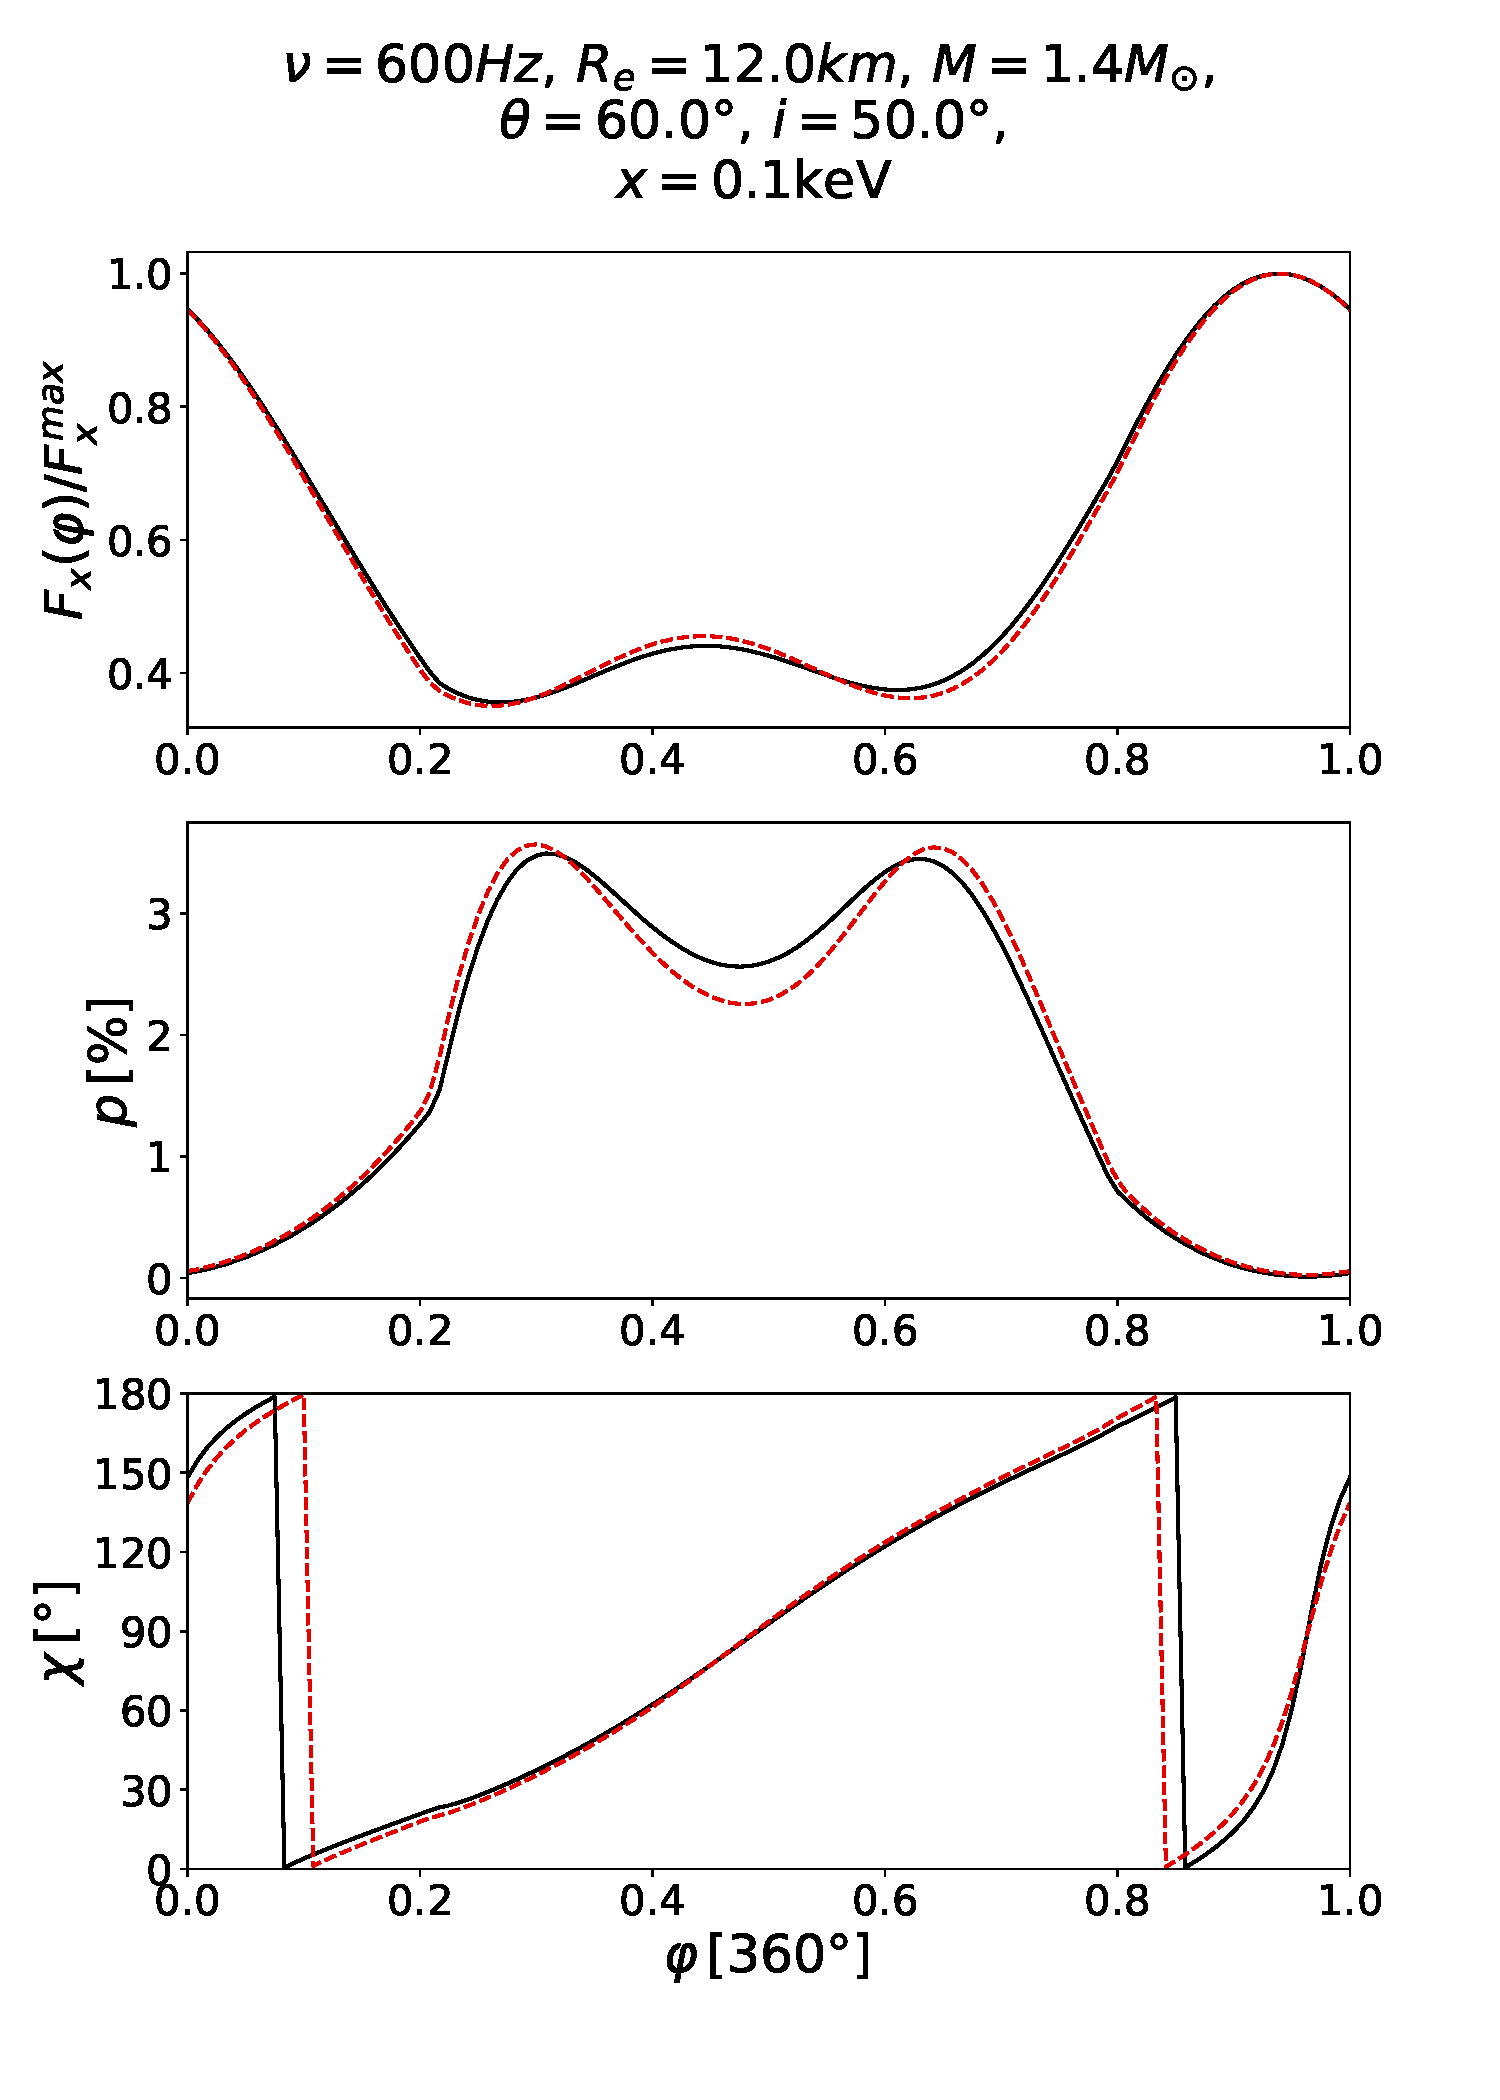
\includegraphics[width=1.1\textwidth]{B0Comb0Ff010.pdf}
					\caption{\small\centering Профили импульса для энергии рэлей-джинсовской области спектра.}
				\end{subfigure}%
				\begin{subfigure}{.45\textwidth}
					\flushright
					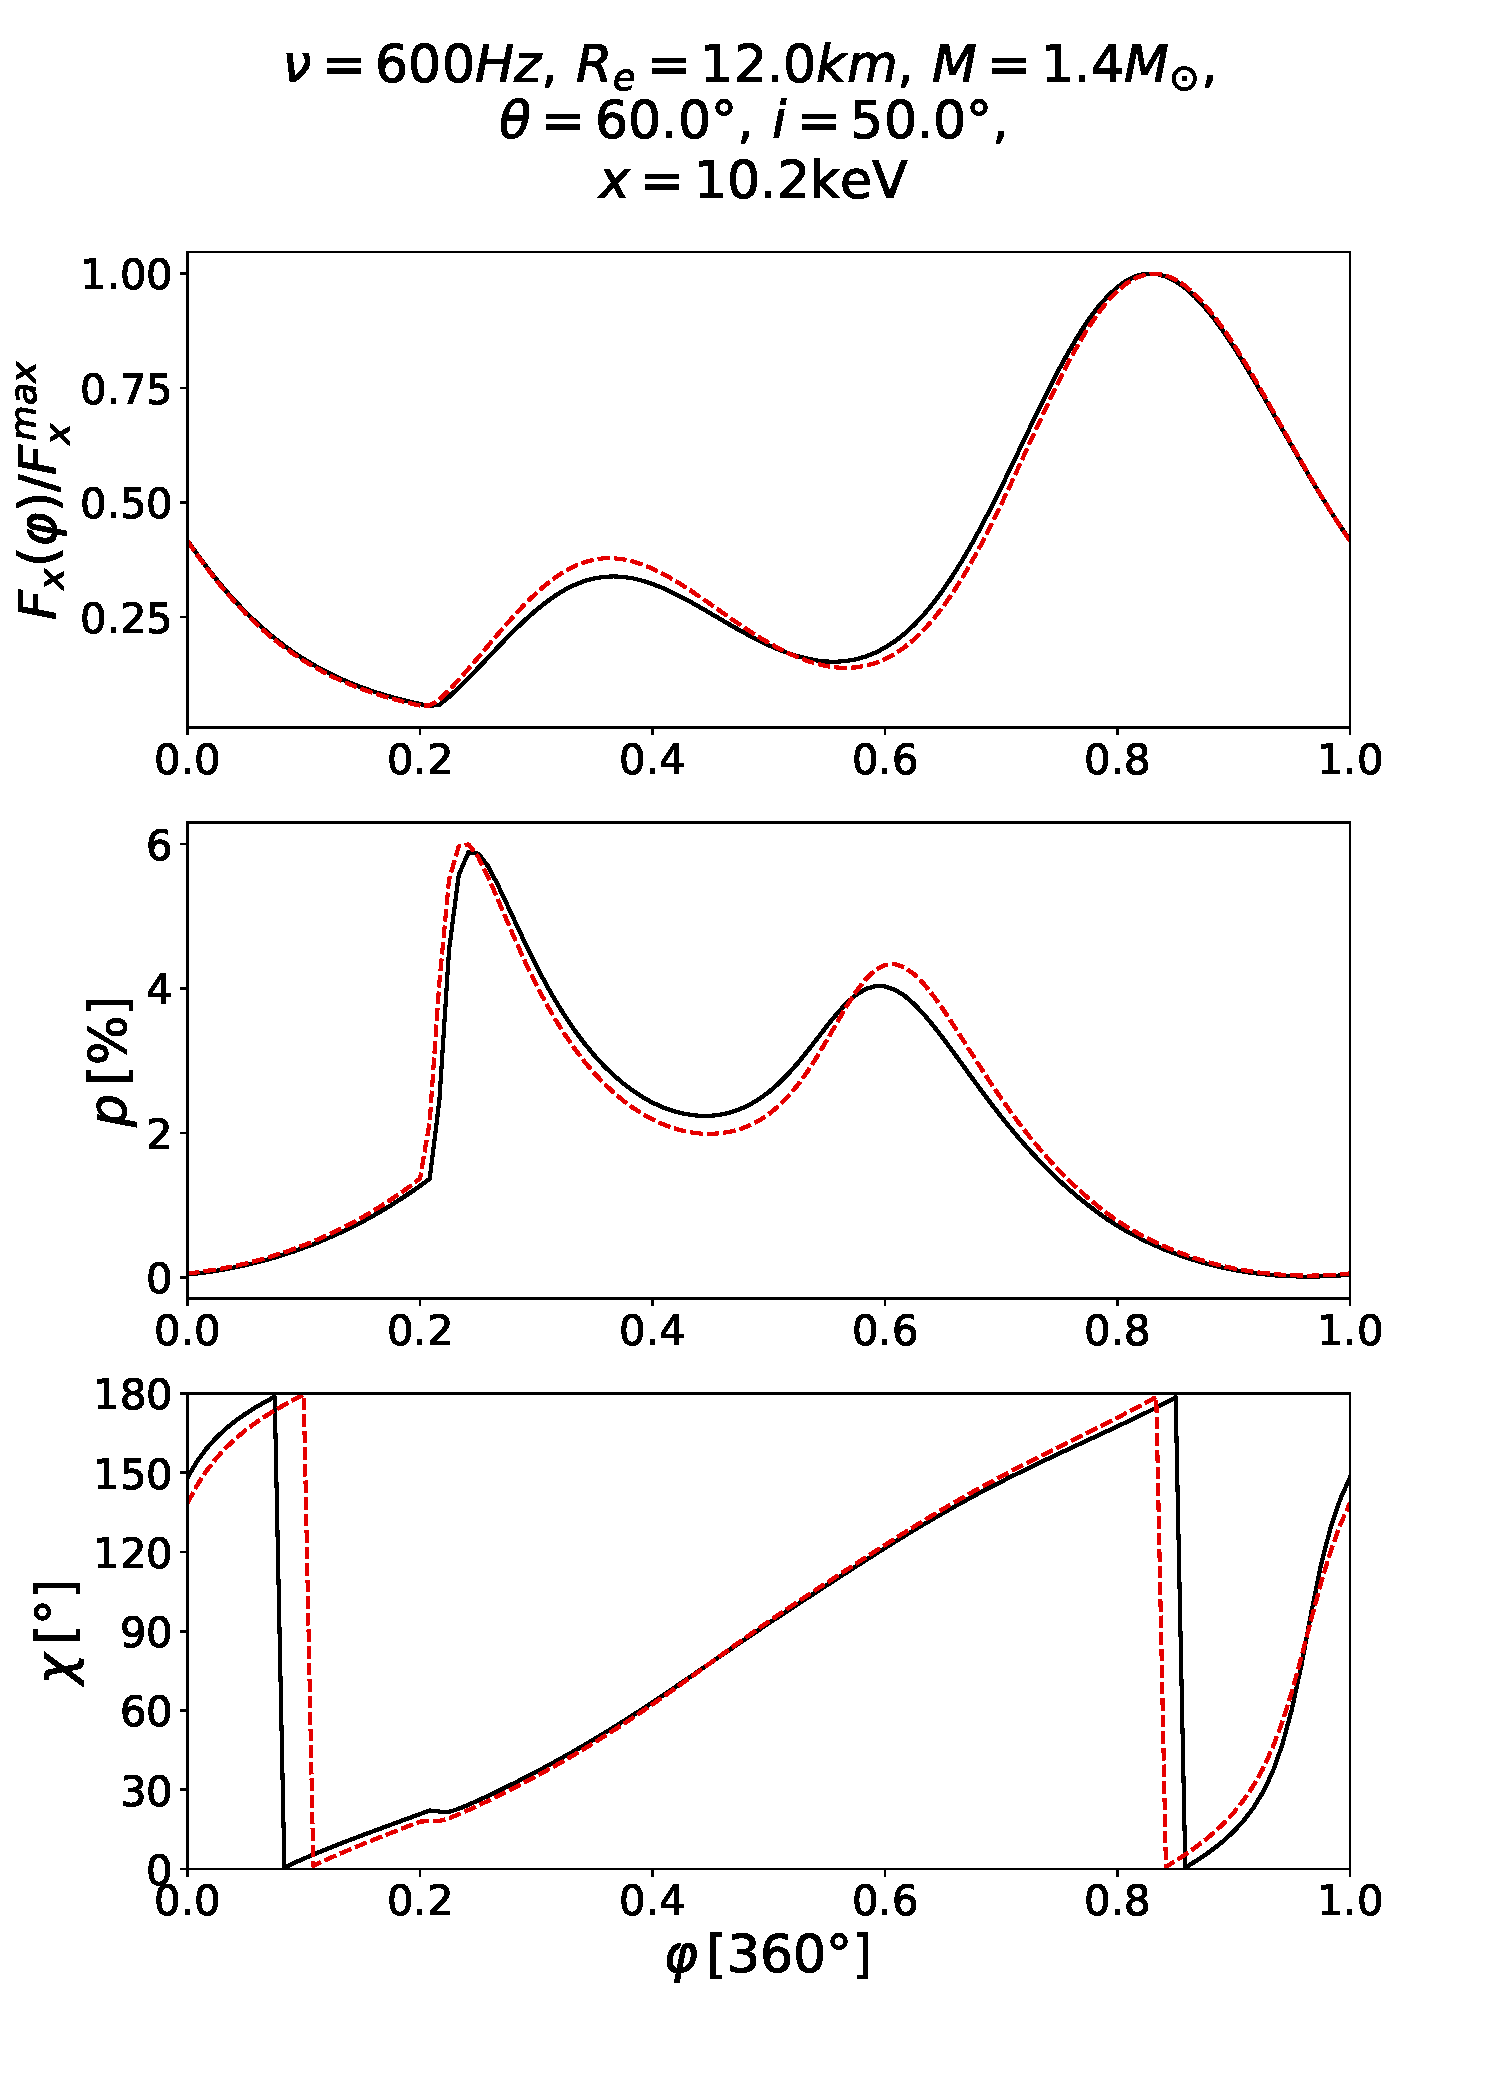
\includegraphics[width=1.1\textwidth]{B0Comb0Ff140.pdf}
					\caption{\small\centering Профили импульса для энергии из виновского хвоста.}
				\end{subfigure}
				\caption{\small
					Показаны отличия моделируемых профилей импульса от таких же, но без учета сплюснутости звезды, для областей спектра с различными спектральными индексами.
					На верхних панелях показан наблюдаемый поток, нормированный на максимум. 
					На средних --- степень поляризации в процентах, а на нижних --- позиционный угол поляризации в градусах от проекции оси вращения пульсара на картинную плоскость против часовой стрелки.
					Черными сплошными линиями обозначен основной результат моделирования, а красными пунктирными проведены кривые полученные для сферической звезды с радиусом $R_e$. 
					Конфигурация углов: $\theta = 60 \degree, \, i = 50\degree$.
					}\label{B0Comp}
			\end{figure}

			 
			Для такой звезды поправки связанные с её формой оказываются значительнее, чем поправки на задержку времени \eqref{eq:timedelay} и  
			отличия между точным выражением для функции $\psi(\alpha)$
			\eqref{eq:bendexact}
			и приближением Белобородова
			\eqref{eq:beloborodovsapproximation}, и это сравнение приведено на рисунке \ref{fig:allComp}.

			\begin{figure}[H]
				\centering
				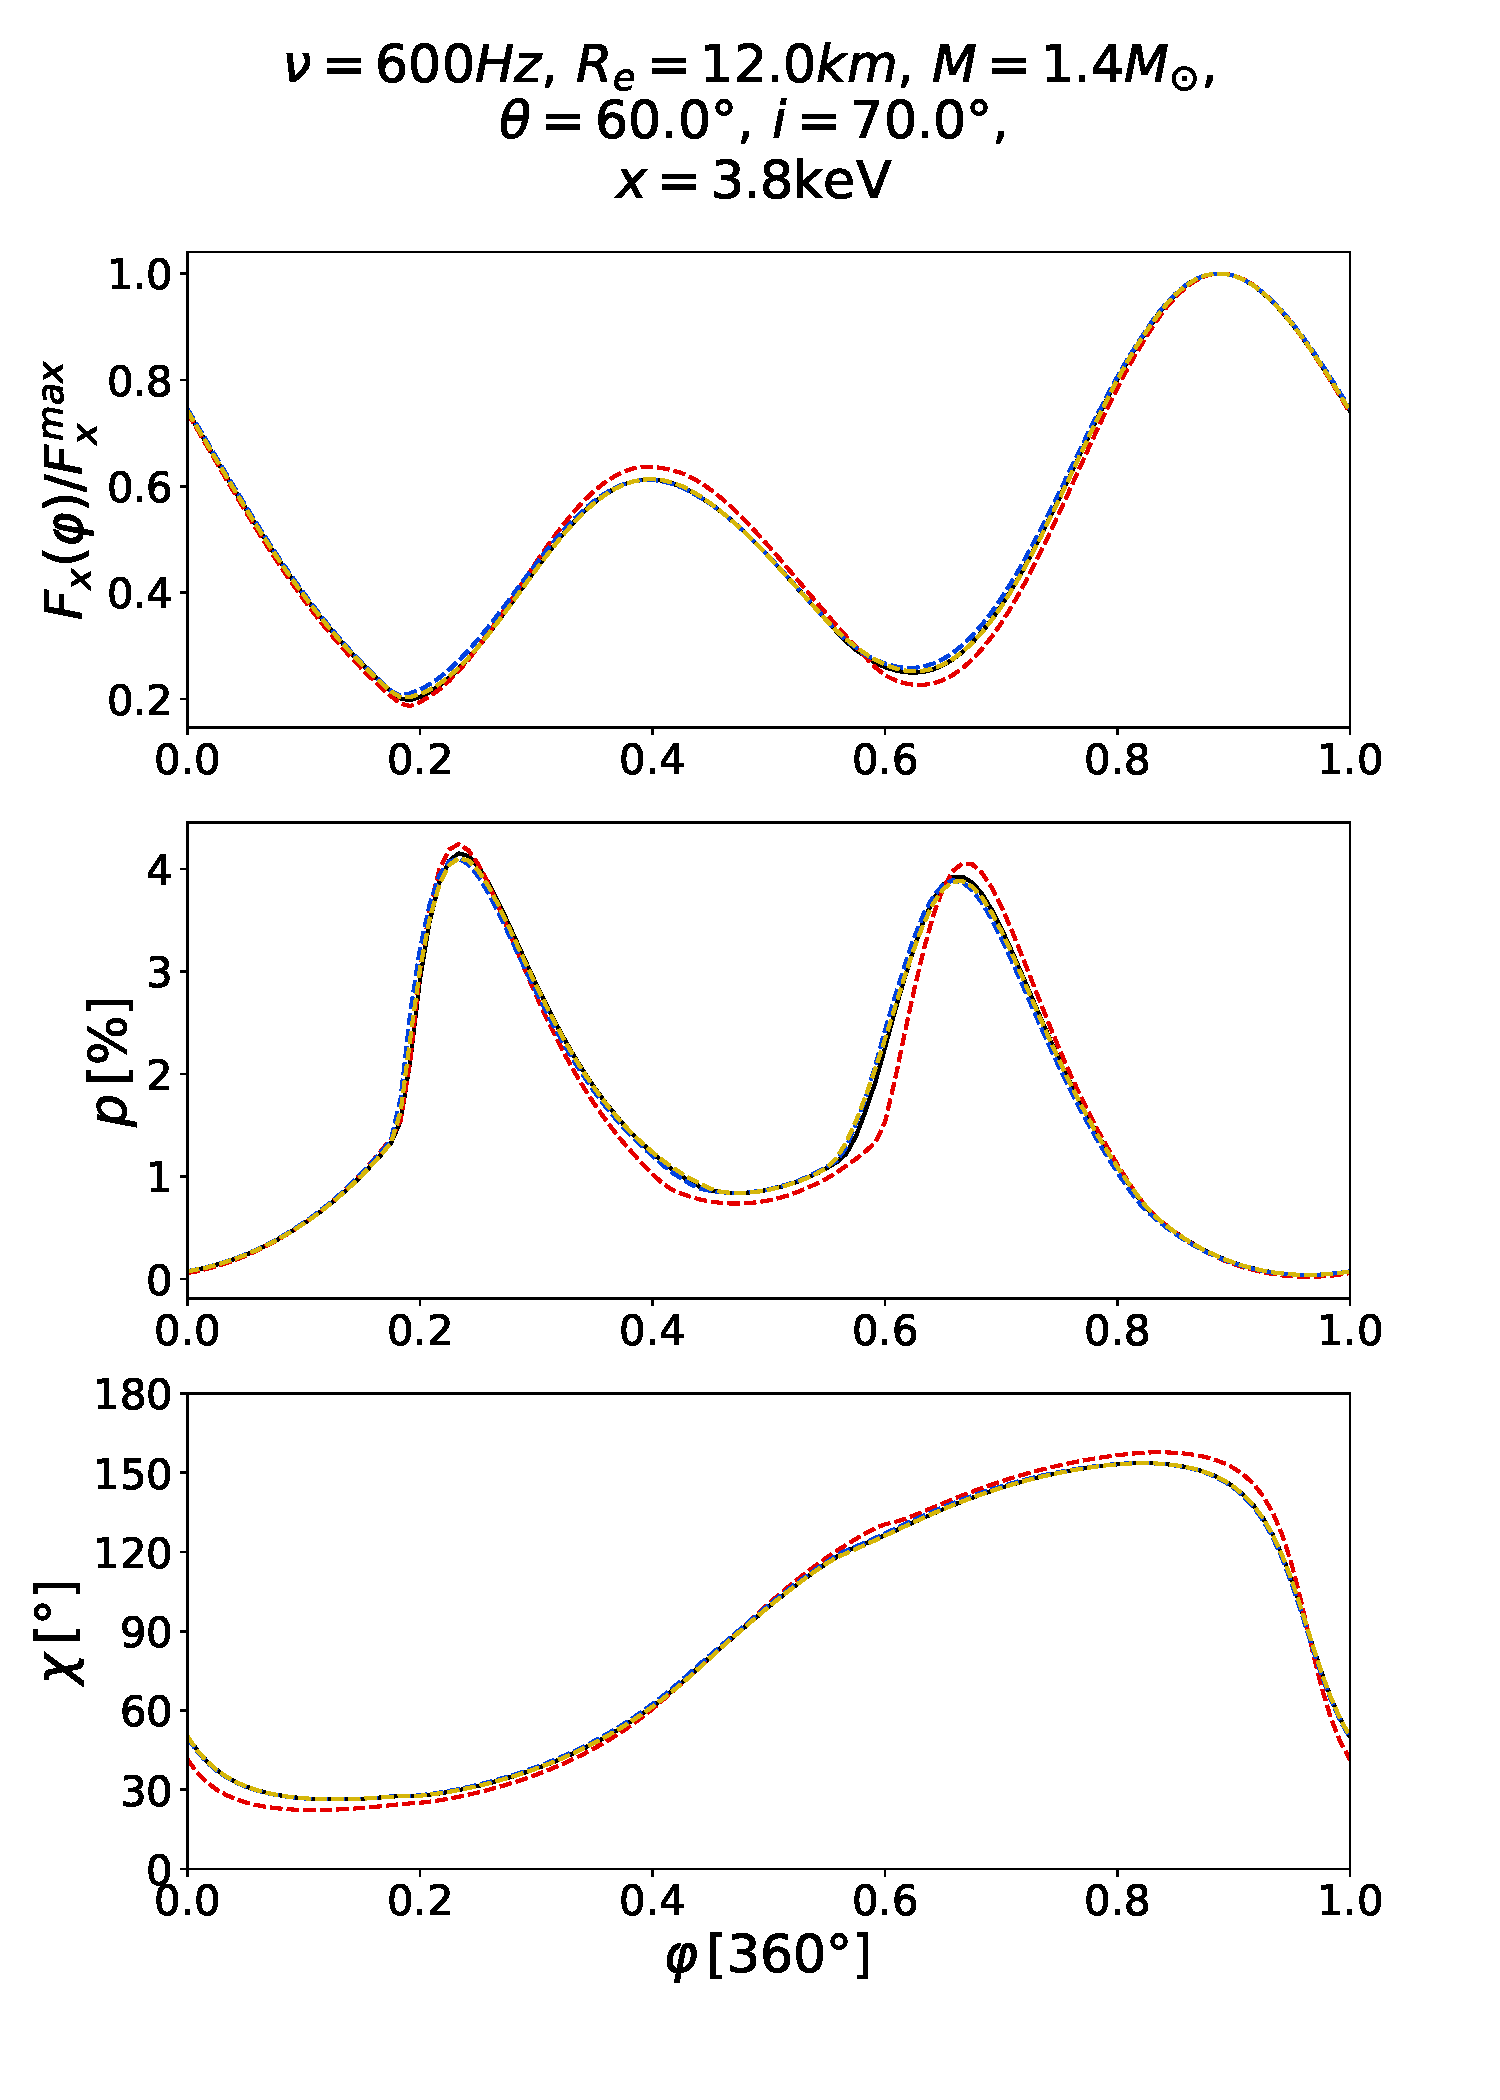
\includegraphics[width=0.8\textwidth]{B10Comb0Ff110.pdf}
				\caption{\small
					Сравнение различных поправок. Графики аналогичны тем, что на рисунке \ref{B0Comp}.
					Профили импульса построены для энергии вблизи максимума чернотельного спектра \eqref{eq:Theta}.
					Конфигурация углов: $\theta = 60 \degree, \, i = 70\degree$.
					Черными сплошными линиями и красными пунктирными так же обозначен основной результат и результат для сферической звезды. 
					Синими пунктирными линиями проведены кривые без учета задержки времени. Желтыми кривыми обозначены кривые полученные в приближении \eqref{eq:beloborodovsapproximation}. 
					}\label{fig:allComp}
			\end{figure}




	\newpage


	\section{Спектральная интенсивность и поляризация излучения в результате комптоновского рассеяния в слое газа в аккреционной ударной волне (внутренняя задача)}\label{Spectra}
		% \textbf{\color{blue} The section names should maybe be different}
		Пятно представляет собой ударную волну горячей плазмы вблизи поверхности звезды.
		Ее можно представить как оптически тонкий слой горячей электронной плазмы. 
		Можно считать, что горизонтальный размер этого слоя много больше его вертикальной высоты, поэтому рассматриваются только фотоны исходящие с верхней поверхности слоя.
		Начальное мягкое излучение с поверхности нейтронной звезды проходит сквозь этот слой и комптонизуется. 
		Спектр этого начального излучения здесь в основном считается тепловым с чернотельной температурой $T_{bb}=\Theta m_ec^2/k$, а степень поляризации начального излучения нулевая. 
		Сверху же на этот слой никакое излучение не приходит.
		Геометрическая толщина слоя $H$ эквивалентна общей томсоновской оптической глубине $\tau_T$. 
		Таким образом можно записать граничные условия для интенсивности излучения
		\be\label{eq:conditions}
			\begin{split}
			 I(\tau=0,x,\mu)&=\frac{2m_e^4c^6x^3}{h^3}\left( e^{ \frac{x}{\Theta_{bb}}} - 1\right)^{-1},\\
			 I(\tau=\tau_T,x,-\mu)&=0.
			 \end{split} \qquad (1>\mu>0)
		\ee   
		Энергия фотона здесь и далее считаются в безразмерных единицах, отнесенных к энергии покоя электрона $x=\frac{h \nu}{m_ec^2}$. 
		Температура $T_{bb}$ соответствует энергиям 1кэВ, или $\Theta_{bb} \approx 0.002 $.
		В этой работе предполагаются такие параметры начальных фотонов, такие как чернотельная форма распределения, отсутствие поляризации и изотропность,
		но эти предположения не влияют на методы расчета комптонизации, поэтому в принципе, в будущем можно рассмотреть и другие формы граничных условий. 


		

		\subsection{Комптоновское рассеяние}\label{sub:CS}
			Для расчета комптонизации были использованы методы и уравнения аналогичные использованным в работах \cite{Poutanen1993} и \cite{Poutanen1996}.
			Горячие электроны плазмы имеют характерное значение кинетической энергии около 50 кэВ, что соответствует безразмерной температуре электронной плазмы $\Theta\approx 0.1$ в единицах энергии покоя электрона $m_ec^2$. 
			Электроны, чьи кинетические энергии сопоставимы с энергией покоя, являются релятивистскими, поэтому их скорости характеризуются Лоренц-фактором $\gamma$. Также рассматривается релятивистское максвелловское распределение электронов по импульсам
			\be 
				\label{eq:Maxwell}
				f_M(\gamma)= \frac{Y e^{-\gamma Y}}{4\pi K_2(Y)},
			\ee
			где $K_2$ --- это вторая модифицированная функция Бесселя, которое характеризуется обратной  безразмерной температурой $Y = 1/ \Theta$. 
			Для ускорения вычислений эта температура считается постоянной по всему объему плазмы. В будущем возможно также рассмотрение двух слоев среды с разными оптическими толщинами и температурами, а так же и в принципе другого закона распределения электронов по энергиям; описанный далее метод практически не опирается на эти предположения. 

			Интенсивность излучения и степень поляризации описываются вектором Стокса $\bm{I}(\tau,x,\mu)$.
			Обычно вектор Стокса имеет в себе 4 параметра, но из-за осевой симметрии и отсутствия всяких источников круговой поляризации, последние два равны нулю и излучение может быть полностью описано лишь двумя параметрами \cite{Chandrasekhar1960}
			\be\bm I =\begin{bmatrix}I\\Q\end{bmatrix}.\ee
			Тогда степень поляризации излучения будет выражаться просто как их отношение $P=Q/I$, а позиционный угол поляризации $\chi$ будет либо $0\degree$, либо $90\degree$ в зависимости от знака $P$. 

			Для описания распространения поляризованного излучения сквозь слой электронной плазмы запишем уравнение переноса излучения в плоско-параллельной среде. 
			В данном случае мы рассматриваем только комптоновское рассеяние и пренебрегаем двухфотонным рождением пар и прочими источниками излучения.
			В таком случае оно выглядит так 
			\be
			\label{eq:transferprime}
			\mu \frac{d \bm I' (z,x,\mu)}{dz} = -  n_e\sigma_{CS}(x)\bm I'(z,x,\mu) + n_e\sigma_T\bm S'(z,x,\mu),
			\ee
			где
			$n_e$ обозначает это электронная концентрация,  
			$\sigma_{CS}(x)$ --- это комптоновское сечение рассеяния, а 
			$\sigma_T$ --- томсоновское сечение рассеяния. 
			Функции обозначены штрихами, потому что зависят от физической глубины $z$ а не оптической $\tau$, но такими функциями пользоваться не удобно.
			Поэтому, используя безразмерные величины \begin{align}
			\bm I=\bm I' \frac{H \sigma_T}{m_e c^3}=\bm I' \frac{\tau_T}{n_e m_e c^3}, \qquad \bm S=\bm S' \frac{H \sigma_T}{m_e c^3},\nonumber\\
			\sigma(x)=\sigma_{CS}(x)/\sigma_T, \qquad \df \tau= \sigma_T n_e dz, \end{align}
			уравнение переноса можно записать в виде  
			\be
			\label{eq:transfer}
			\mu \frac{d \bm I (\tau,x,\mu)}{\df \tau} = -  \sigma(x)\bm I(\tau,x,\mu) + \bm S(z,x,\mu),
			\ee
			где функция источников $\bm S$ тоже является вектор-столбцом из двух параметров и  
			может быть выражена через усредненную по азимуту функцию перераспределения $\bm{R}$, вычислению которой посвящено приложение \ref{redistr}, 
			\be
			\label{eq:Source}
			\bm S(\tau,x,\mu)= x^2 \int_0^\infty \frac{\df x_1}{x_1^2} \int_{-1}^1 \df \mu_1 
			\bm{R}(x,\mu,x_1,\mu_1)\bm{I}(\tau,x_1,\mu_1).
			\ee
			Это уравнение можно коротко записать как применение интегрального оператора $ \hat{\bm{R}}$
			\be
			\label{eq:Rop}
			\bm{S}=\hat{\bm{R}}\bm{I}.
			\ee
			Интегродифференциальное уравнение \eqref{eq:transfer} решается разложением $\bm{I}$ в ряд по порядкам рассеяния
			 \be
			 \bm{I}=\sum_{k=0}^\infty \bm{I}_k,
			\ee
			где $\bm{I}_k$ --- это вектор Стокса, описывающий фотоны, рассеянные $k$ раз \cite{Sunyaev1985}.
			Каждая из этих функций так же может быть выражена как интегральный оператор от некоторой $k$-ой функции источников $\bm{S}_k$
			\be
			\label{eq:Sop}
			 \bm{I}_k=\hat{\bm{\Sigma}}\bm{S}_k,
			\ee
			что расшифровывается как
			 \be
			 \hat{\bm{\Sigma}}\bm{S}=\int_{\tau_TH(\mu)}^\tau \frac{\df \tau'}{\mu} \bm{S}(\tau',x,\mu) e^{\sigma(x)\frac{\tau'-\tau}\mu},
			\ee 
			где $H(\mu)$ --- это ступенчатая функция Хевисайда. 
			Из граничных условий \eqref{eq:conditions} получаем начальный вектор Стокса $\bm{I}_0$, описывающий нерассеянные фотоны в слое плазмы
			\be
			\bm{I}_0(\tau,x,\mu)=I_{in}(x) e^{-\sigma(x)\tau/\mu}\begin{bmatrix}1\\0\end{bmatrix},
			\ee 
			а вектор Стокса для $k$-ого рассеяния получается из вектора Стокса для предыдущего последовательным применением \eqref{eq:Rop} и \eqref{eq:Sop}
			\be
			\bm{I}_k=\hat{\bm{\Sigma}}\hat{\bm{R}}\bm{I}_{k-1}
			\ee

			Затем можно вычислить степень поляризации исходящего потока   
			\be
			p(x,\mu)=100\%\frac{I(\tau_T,x,\mu)}{Q(\tau_T,x,\mu)},
			\ee
			а затем и наблюдаемые величины потока  $xF_x$ и его поляризации по формулам 
			\eqref{eq:flux},
			\eqref{eq:Ptot} и \eqref{eq:chitot} 
			из раздела \ref{Outer}.

			В результате спектр должен получаться относительно плоским \cite{Poutanen2003,Poutanen2008},  и с учетом этого подбираются параметры  $\tau_T$ и $\Theta$. 
			Наиболее похожие спектры получаются при $1<\tau_T<2$ и $0.06<\Theta<0.1$.
			На рисунках \ref{fig:Comp0},
			\ref{fig:Comp2}, \ref{fig:Comp4},
			\ref{fig:Comp1}
			и \ref{fig:Comp3} представлены результаты расчета комптоновского рассеяния для различных параметров атмосферы $\tau_T$ и $\Theta$. 

			\newpage
			\begin{figure}[H]
				\centering
				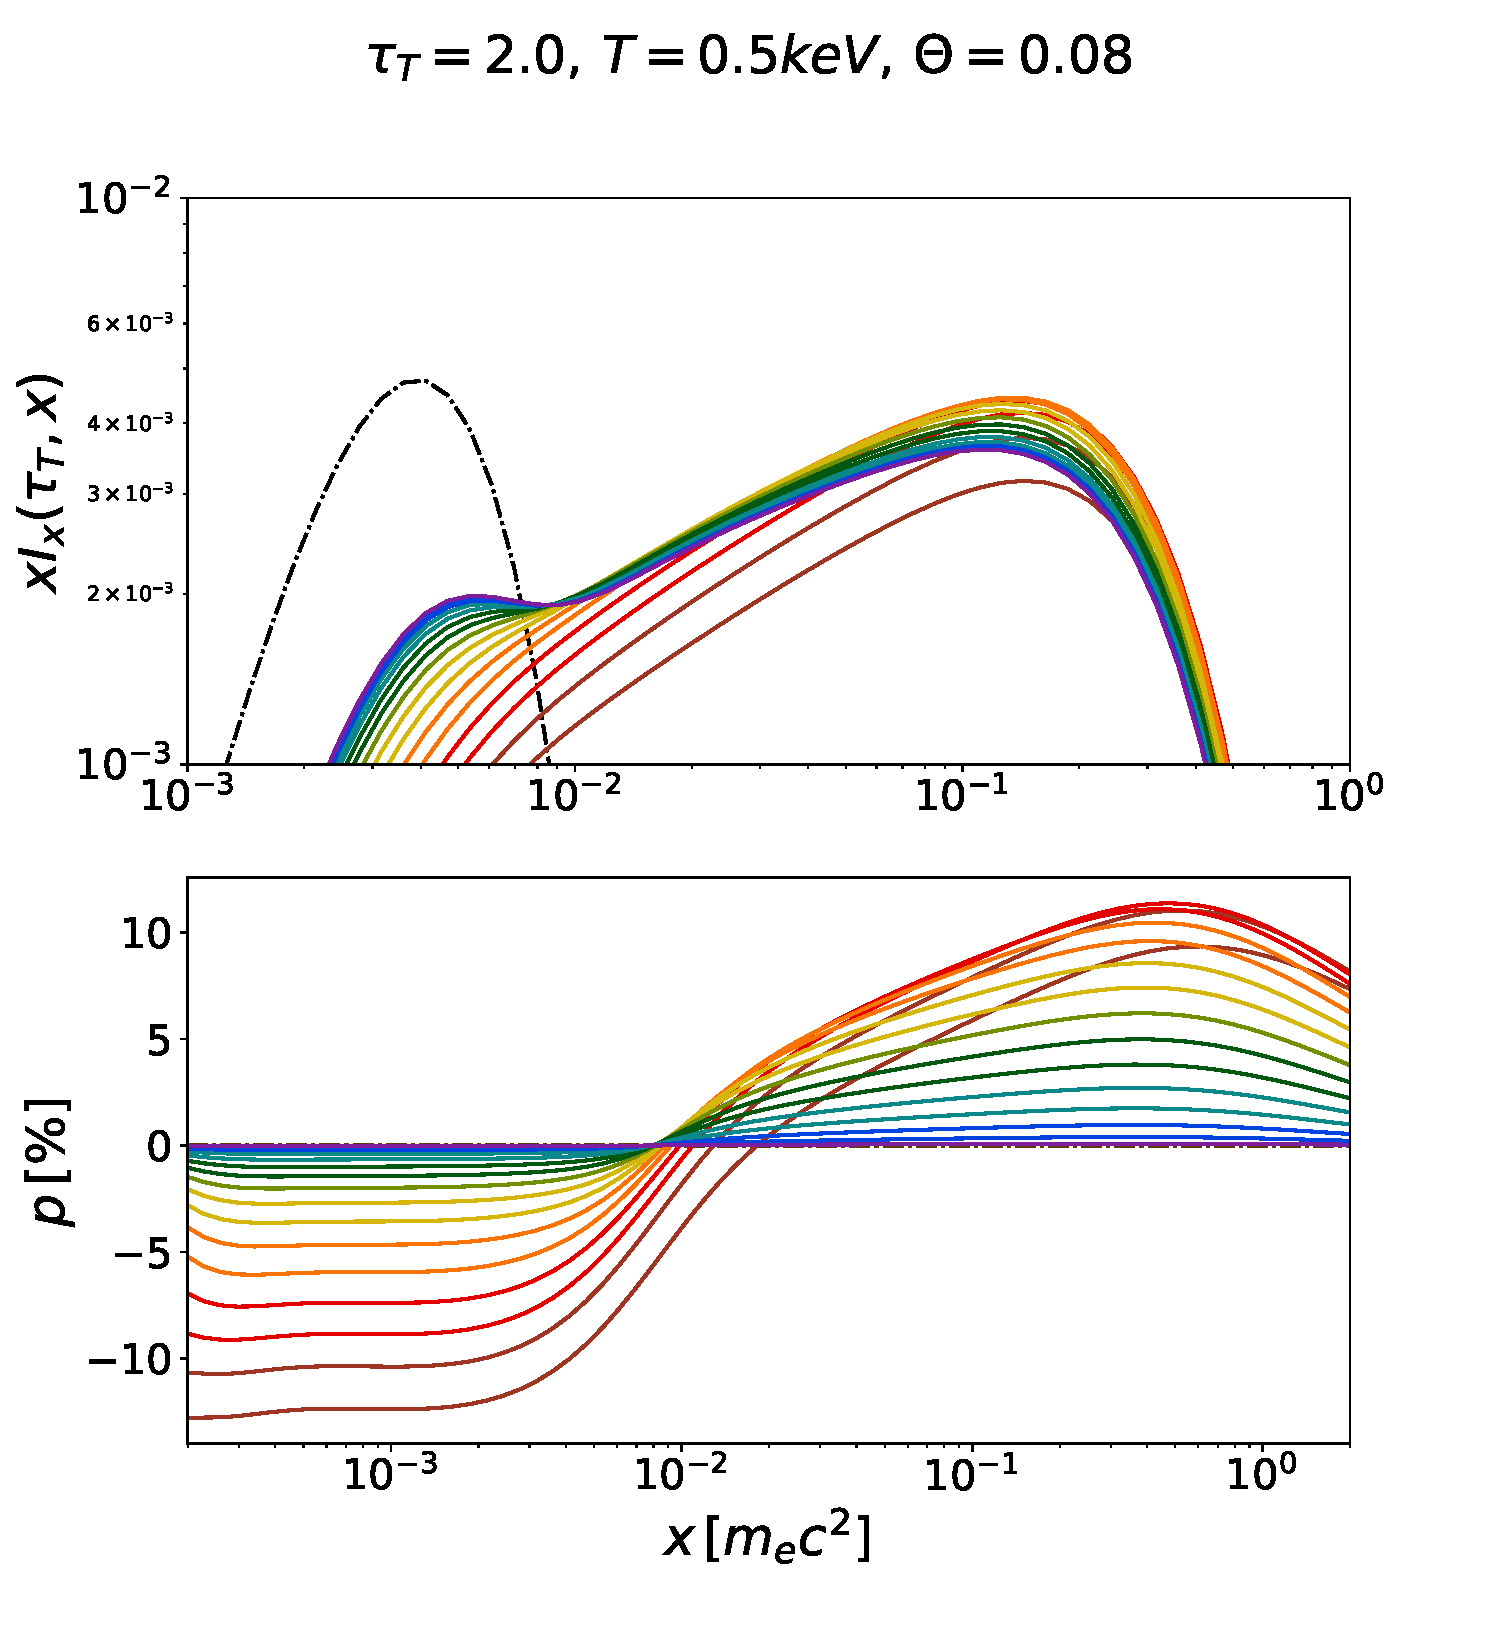
\includegraphics[width=0.8\textwidth]{CM2zAll.pdf}
				\caption{\small
					Результат моделирования спектра излучения рассеянного в слое
					 релятивистских электронов с температурой $\Theta=0.08$
					 оптической толщины $\tau_T=2$. 
					Цвета кривых соответствуют разным зенитным углам, под которым выходит излучение. 
					Каждый цвет соответствует косинусу зенитного угла $\mu$ равному положительному корню одного полинома Лежандра, таким сетка по зенитному углу $z$ близка к равномерной. 
					На верхнем графике показаны величины спектральной интенсивности $xI_x(\mu)$ в произвольных величинах, а на нижнем --- отношение параметров Стокса $P=Q/I$ в процентах. 
					Таким образом отрицательная степень поляризации $P$ соответствует повороту плоскости поляризации на 90\degree.
					Чернотельное начальное излучение имеет температуру $T_{bb}=0.5$ кэВ и его спектр показан темно-коричневым штрих-пунктиром на верхней панели.
					Этот набор параметров и обозначений принимается основным для графиков в этом пункте. 
				}\label{fig:Comp0}
			\end{figure}
			\newpage
			\begin{figure}[H]
				\centering
				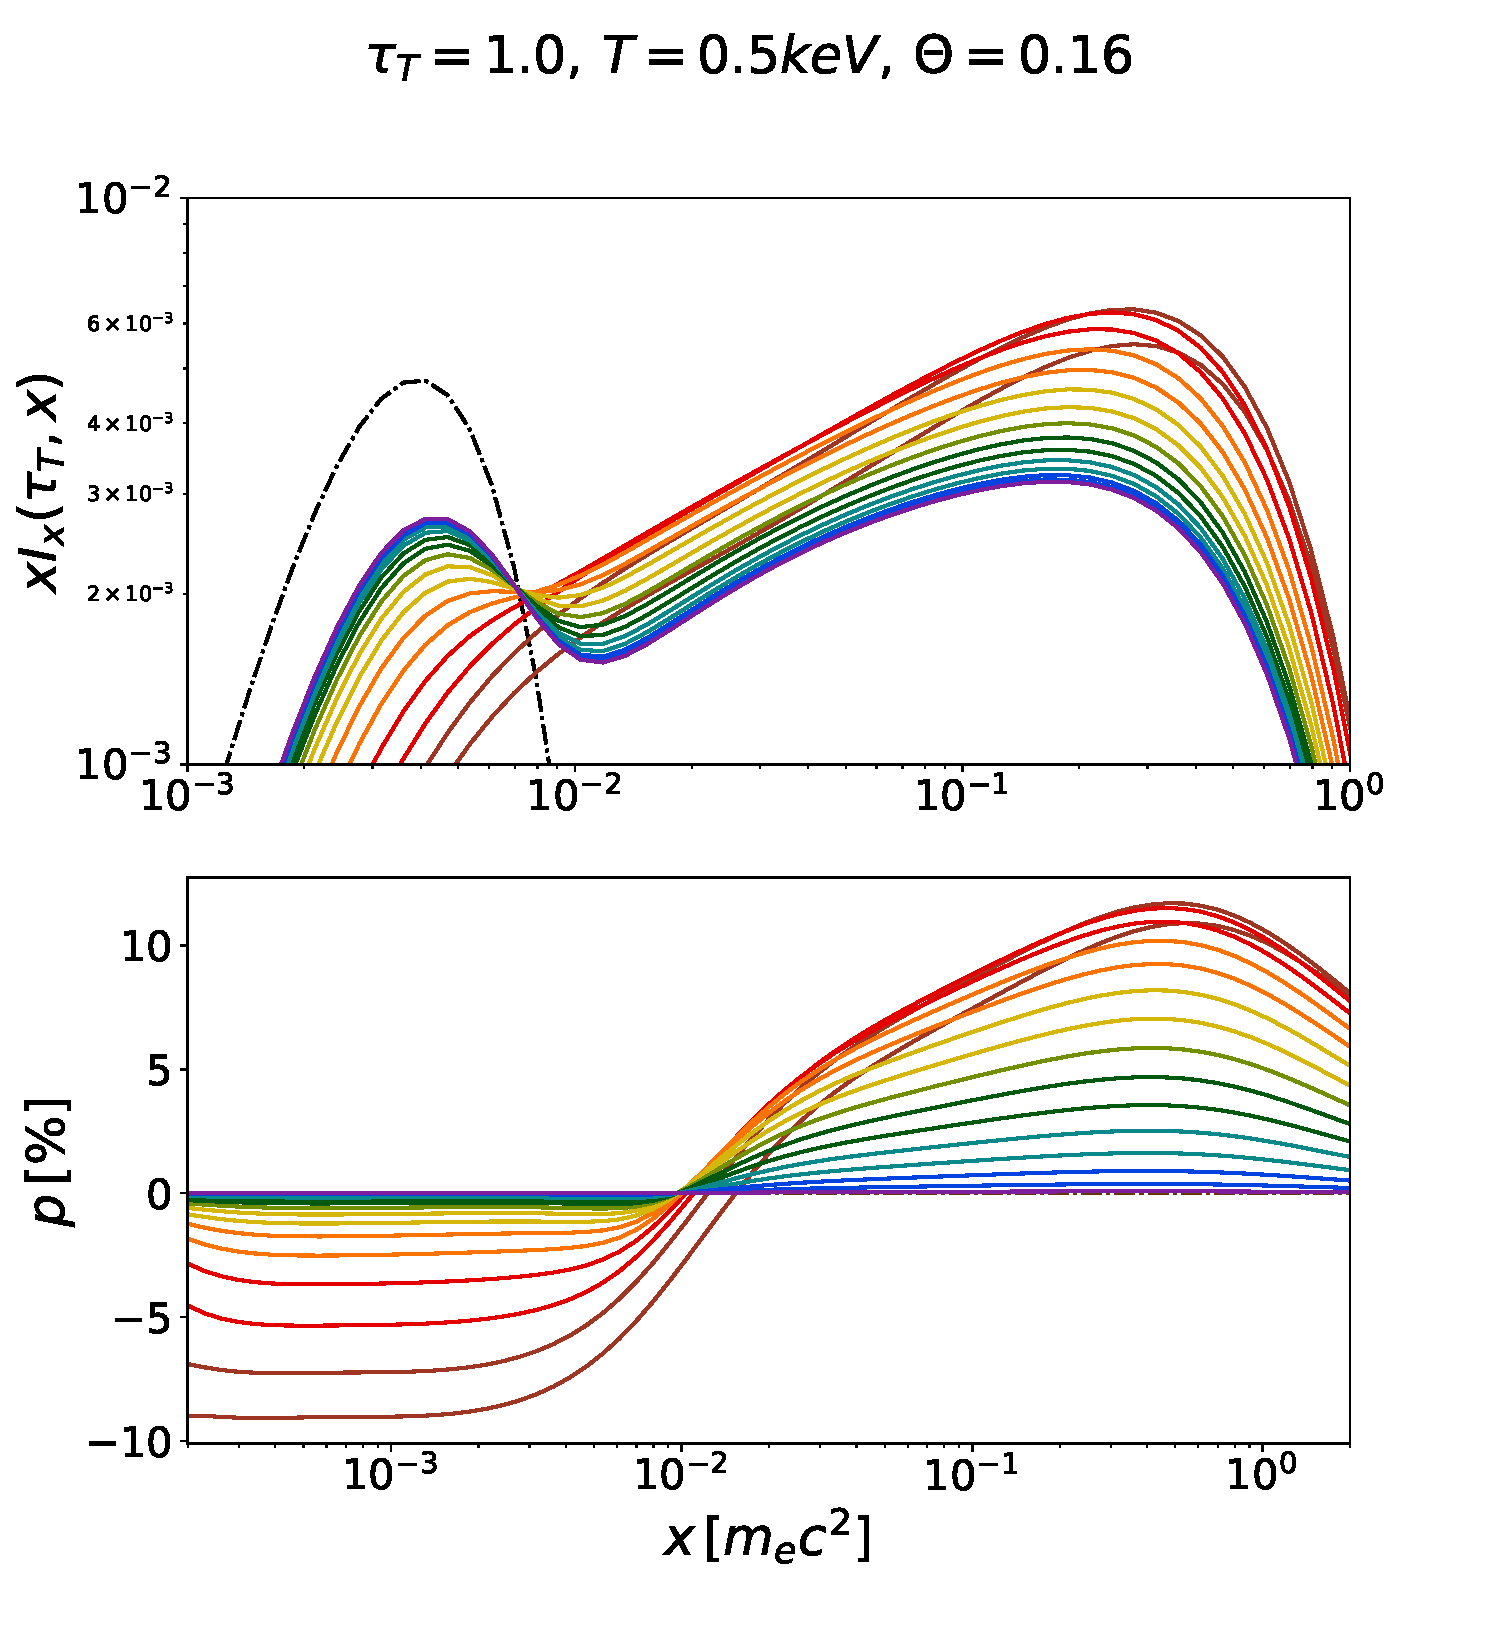
\includegraphics[width=0.8\textwidth]{CM1zAll.pdf}
				\caption{\small
				Результат моделирования спектра излучения рассеянного в слое
			    оптической меньшей оптической толщины $\tau_T=1$,  
			    но большей температуры $\Theta=0.16$
				}\label{fig:Comp2}
			\end{figure}
			\newpage
			\begin{figure}[H]
				\centering
				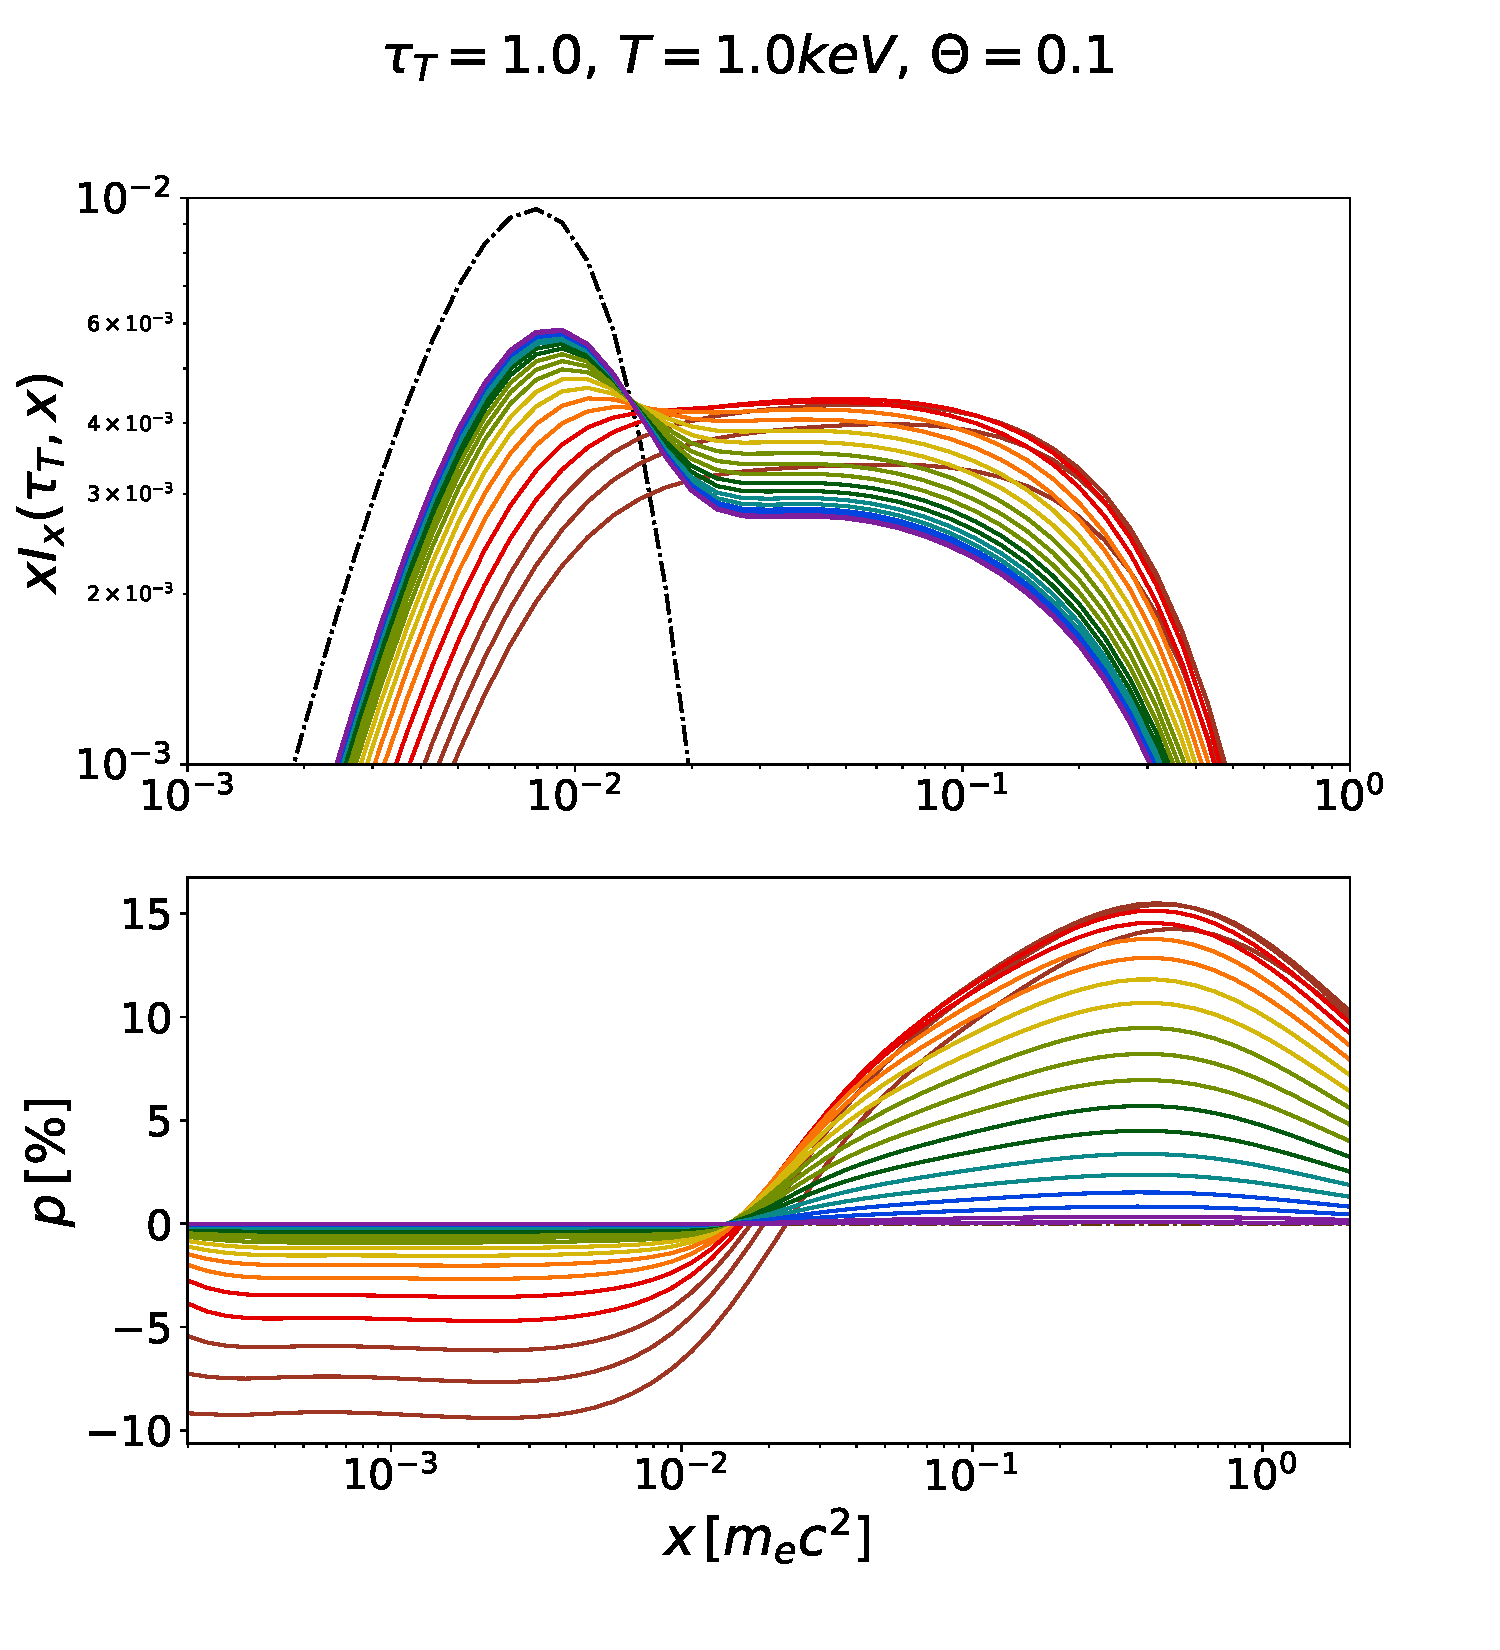
\includegraphics[width=0.8\textwidth]{C0zAll.pdf}
				\caption{\small
				Результат моделирования спектра излучения рассеянного в слое 
					 релятивистских электронов с температурой $\Theta=0.1$ оптической толщины $\tau_T=1$.
					Температура начального чернотельного излучения увеличена до 1 кэВ.
				}\label{fig:Comp4}
			\end{figure}
			\newpage
			\begin{figure}[H]
				\centering
				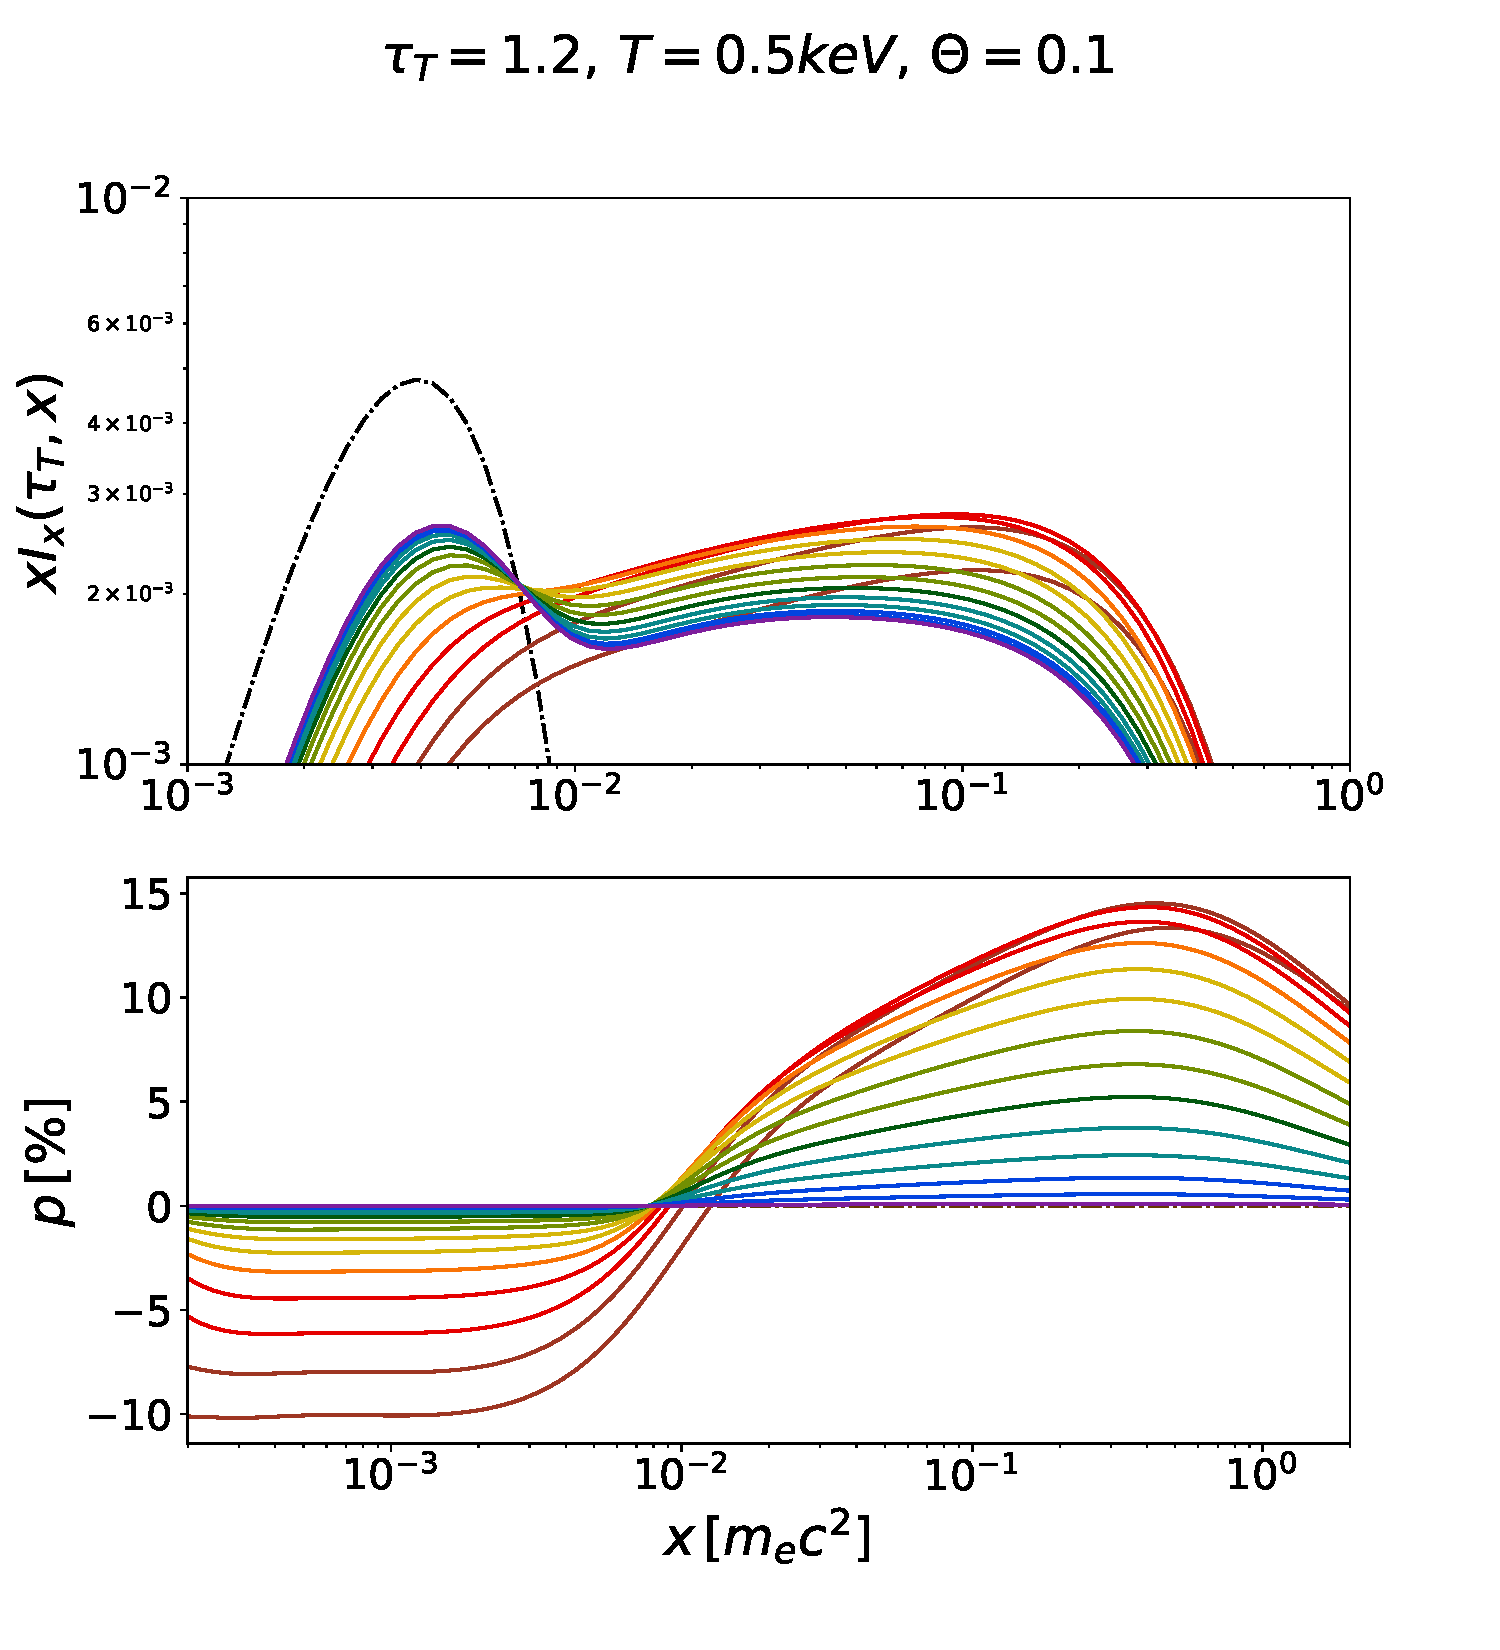
\includegraphics[width=0.8\textwidth]{CM10zAll.pdf}
				\caption{\small
					Результат моделирования спектра излучения рассеянного в слое
					оптической толщины $\tau_T=1.2$ с температурой электронов $\Theta=0.1$. 
				}\label{fig:Comp1}
			\end{figure}
			\newpage





		\subsection{Томсоновское рассеяние}\label{sub:TS}
			В этом разделе рассмотрим приближение, основанное на модели классического томсоновского рассеяния с постоянным относительным сдвигом по энергии, предложенное в \cite{Viironen2004}.
			При рассеянии на электронах плазмы с безразмерной температурой $\Theta$ квант света, имеющий энергию $E$, намного меньшую, чем кинетическая энергия этого электрона, в среднем приобретает энергию \cite{Rybicki1979} \be\label{eq:energyshift}
				\frac{\Delta x}{x} \approx 4\Theta - x\ee % -x oili
			Таким образом, при каждом рассеянии энергитический спектр равномерно сдвигается по логарифмической шкале энергий пока не достигнет энергий порядка $\Theta$, характерных для электронов плазмы. На энергиях выше $4\Theta$ поляризация просто исчезает. 

			Зависимость интенсивности и поляризации от направления исходящих от слоя фотонов рассчитывается в приближении томсоновского рассеяния. 
			Используемый метод расчета параметров Стокса для $k$ раз рассеянных фотонов аналогичен методу, описанному в 
			\cite{Sunyaev1985}.
			Интенсивность излучения раскладывается на две компоненты $I^l$ и $I^r$ с векторами электрической напряженности колеблющимися в плоскости, образованной векторами $\bm{k_0} $ и $ \bm n$, и, соответственно, перпендикулярно ей (вдоль $\bm{k_0} \times \bm n$).
			Для каждой из этих компонент выполняются граничные условия \eqref{eq:conditions}.
			Тогда интенсивности для ни разу не рассеянных фотонов в любой области спектра задаются формулой 
			\be
				I_0^l(\tau,\mu)=I_0^r(\tau,\mu)=I_0 e^{-\frac{\tau}{\mu}}.
			\ee
			С произвольной начальной нормировочной интенсивностью $I_0$.
			А интенсивности для фотонов, испытавших $k$ рассеяний вычисляются рекуррентно по формулам
			\be
				I^l_{k} (\tau,\mu) = \int_{\tau_TH(\mu)}^\tau \frac{\df \tau'}{\mu}  \left(
					A_k(\tau')\left(1-\mu^2\right)+\left(B_k(\tau')+C_k(\tau')\right)\mu^2
				\right)e^{\frac{\tau'-\tau}\mu},
			\ee
			\be
				I^r_k (\tau,\mu) = \int_{\tau_TH(\mu)}^\tau \frac{\df \tau'}{\mu}  \left(B_k(\tau')+C_k(\tau')
				\right)e^{\frac{\tau'-\tau}\mu},
			\ee
			где величины $A_k$, $B_k$ и $C_k$ вычисляются следующим образом
			$$
				A_k(\tau') = \frac34\int_0^1  \left(1-\mu'^2\right)\left(I_{k-1}^l(\tau',\mu')+I_{k-1}^l(\tau',-\mu')\right) \df \mu',
			$$\be
				B_k(\tau') = \frac38\int_0^1  \mu'^2 \left(I_{k-1}^l(\tau',\mu')+I_{k-1}^r(\tau',-\mu')\right) \df \mu',
			\ee$$
				C_k(\tau') = \frac38\int_0^1  \left(I_{k-1}^r(\tau',\mu')+I_{k-1}^r(\tau',-\mu')\right) \df \mu'.
			$$
			В конечном счете, параметры Стокса получаются соответственно путём сложения и вычитания двух компонент интенсивности 
			\be
				I_{k}(\tau,\mu)=I^l_{k}(\tau,\mu)+I^r_{k}(\tau,\mu),
			\ee\be
				Q_{k}(\tau,\mu)=I^l_{k}(\tau,\mu)-I^r_{k}(\tau,\mu).
			\ee
			Наконец, можно записать вектор Стокса исходящего излучения для  всех порядков рассеяния
			\be
				\bm I_{k}(\mu)=\begin{bmatrix}I_{k}(\tau_T,\mu)\\Q_{k}(\tau_T,\mu)\end{bmatrix}.
			\ee
			Зависимость от энергии получается с учетом соотношения \eqref{eq:energyshift}
			путём суммирования вектора Стокса для всех порядков рассеяния
			\be
				\bm I(x_0,\mu)=\sum_{k=0}^{\infty}\frac{\bm I_{k}(\mu)}{I_0} I\left(\tau=0,x_k,\mu\right) \frac{x}{x_k},
			\ee
			где, согласно \eqref{eq:energyshift}, \be
				x_{k-1}-x_k=4\Theta x_k - x_k^2.
			\ee


			На рисунках \ref{fig:specificanglecomperison} и \ref{fig:allcomparison} представлены сравнения результатов моделирования исходящего спектра для этого приближения и для точного расчета комптоновского рассеяния, описанного в разделе \ref{sub:CS}. 
			В целом кривые степени поляризации имеют похожую форму, но с некоторыми существенными различиями. В томсоновском приближении процент поляризованного излучения как правило значительно выше (до двух раз), чем в комптоновском почти на всем промежутке рентгеновского спектра. 
			Также можно отметить, что степень поляризации излучения меняет знак с отрицательного на положительный при больших энергиях, чем это получается при расчете комптоновского рассеяния. 
			Тем не менее, в обоих случаях, минимальная степень поляризации попадает  в область спектра, предполагаемую для наблюдения космическими аппаратами \cite{XIPE}, что может затруднить наблюдение параметров поляризаци. 
			В томсоновском приближении на энергии порядка $4\Theta$ и выше фотоны просто не рассеиваются, поэтому степень поляризации в этой области спектра просто равна нулю. 
			При расчете комптоновского рассеяния на этих энергиях существует положительная поляризация, однако, это не имеет значения, так как в настоящее время точные наблюдения потока и его поляризации на таких высоких энергиях попросту не возможны.   
			\newpage
			\begin{figure}[H]
				\centering
				\begin{subfigure}{.5\textwidth}
					\centering
					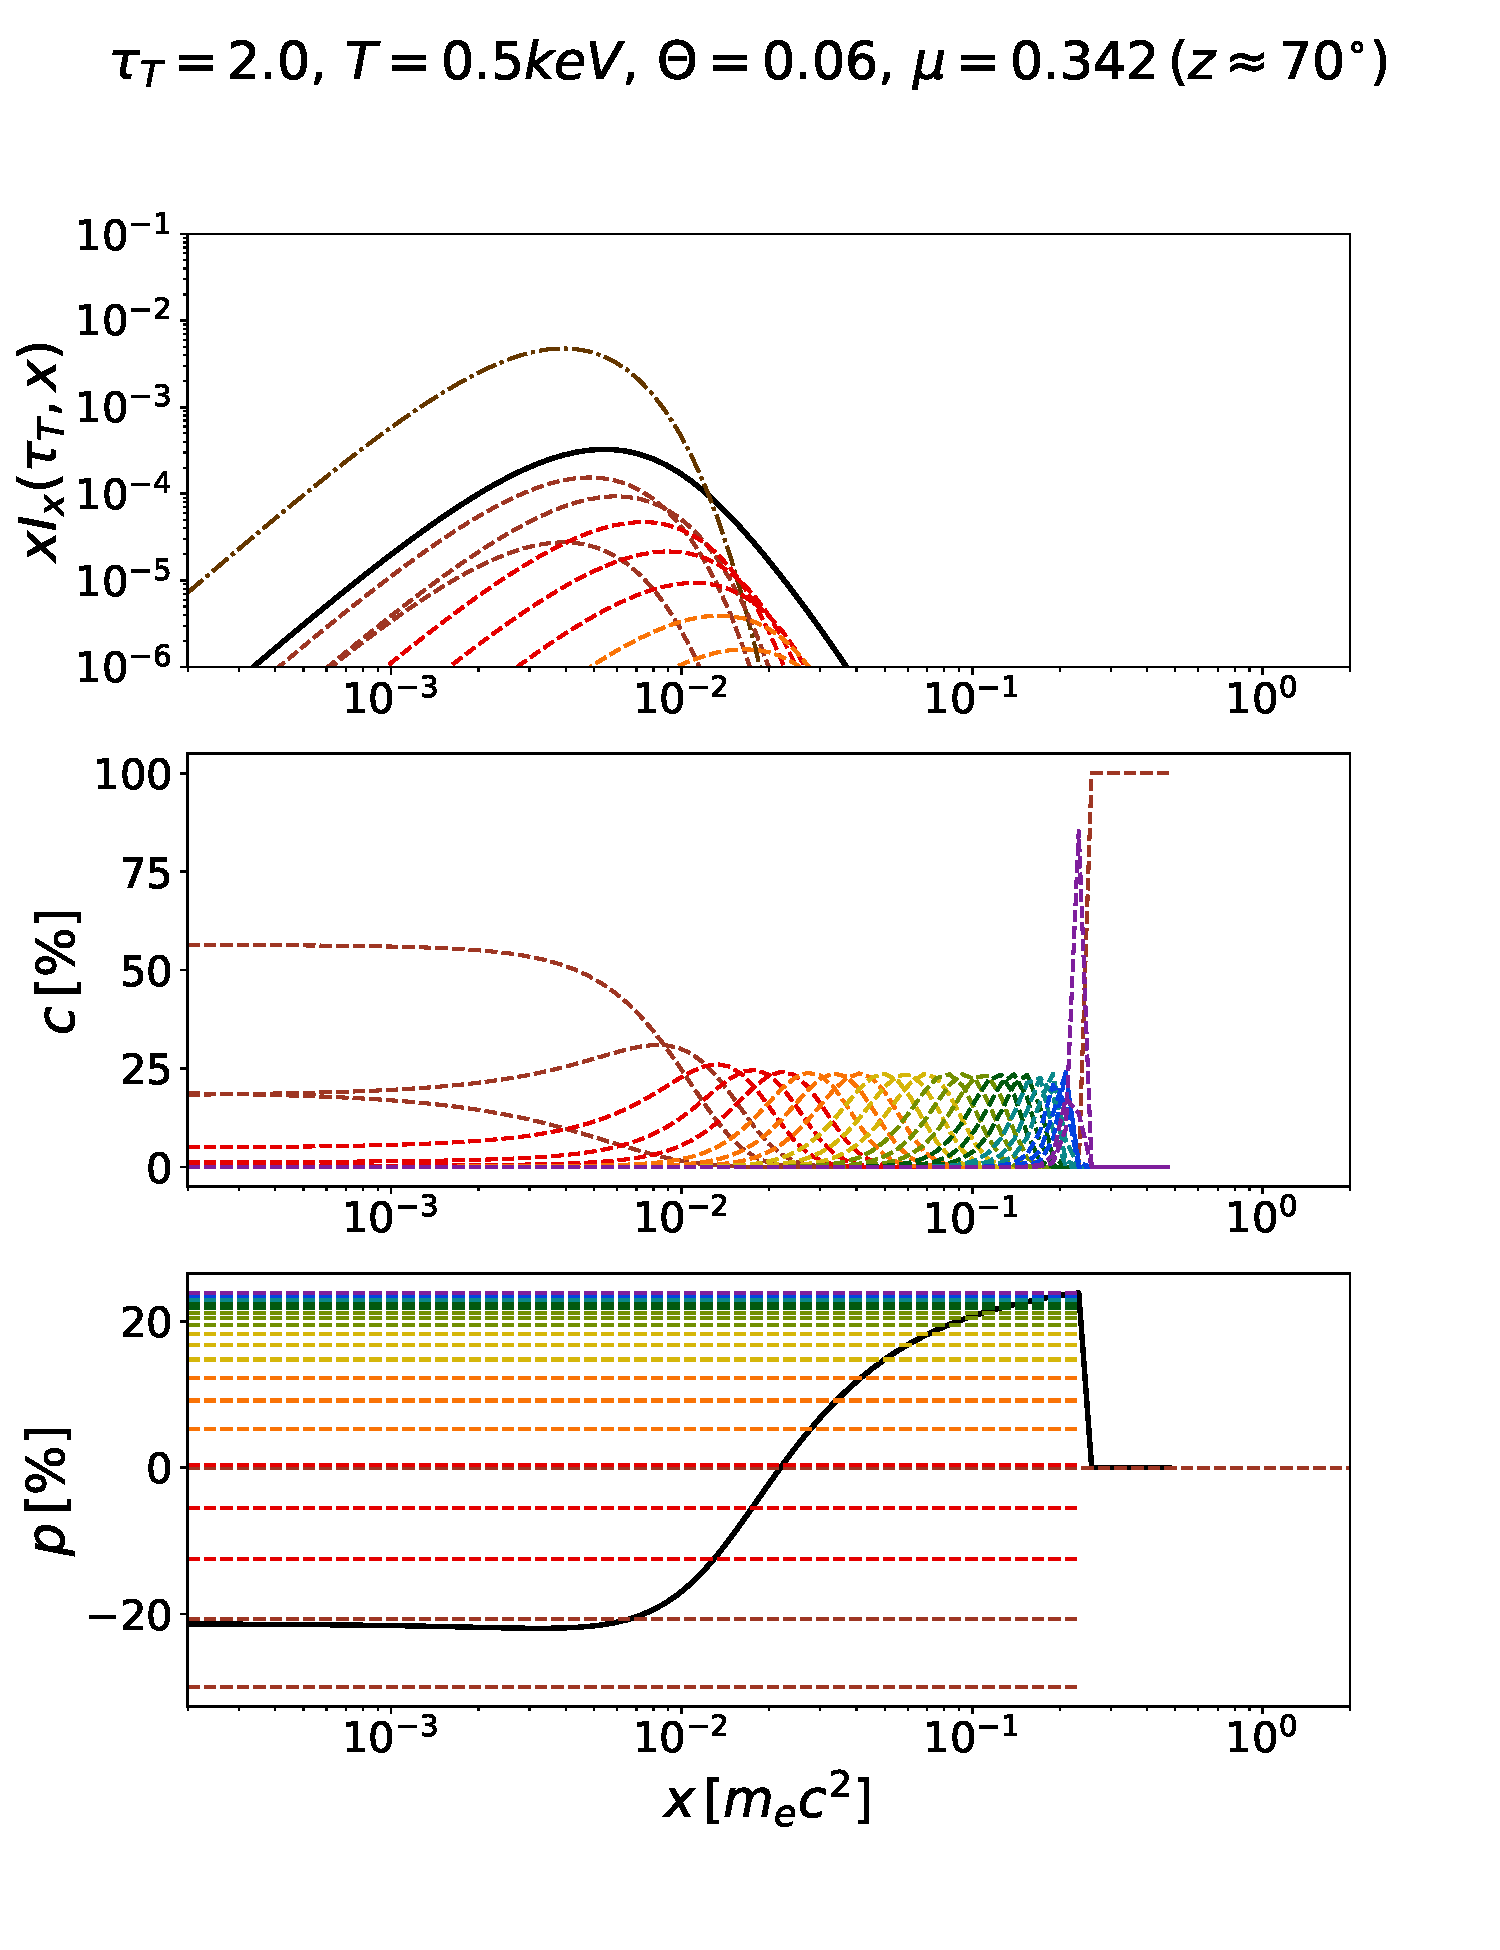
\includegraphics[width=\textwidth]{TM9z70.pdf}
					\caption{\small\centering Поляризация в томсоновском приближении.}
				\end{subfigure}%
				\begin{subfigure}{.5\textwidth}
					\centering
					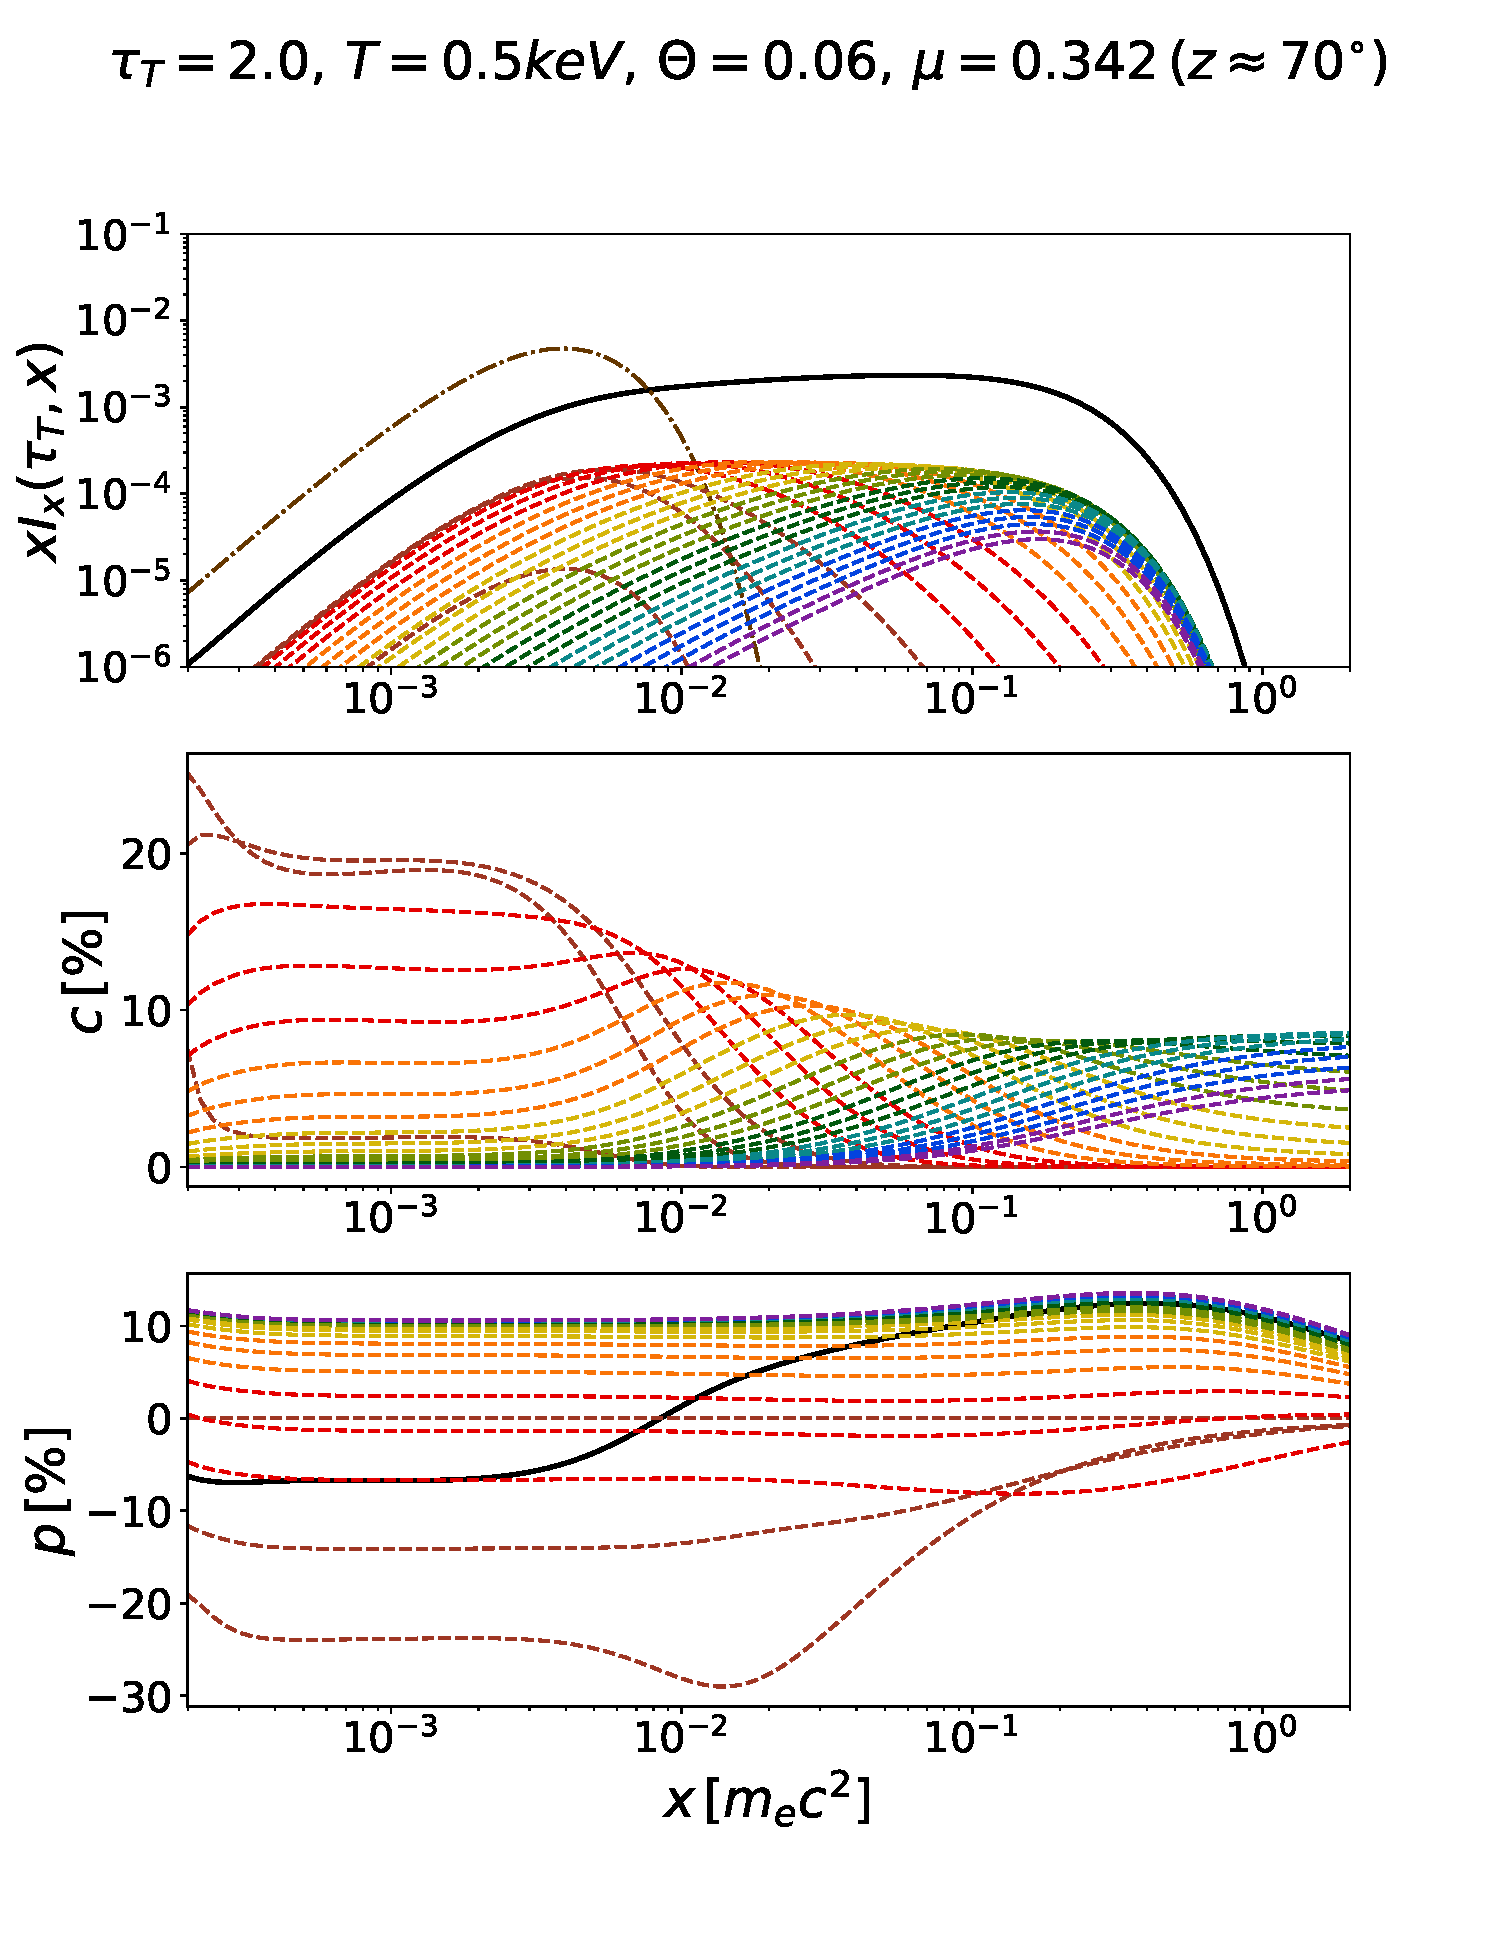
\includegraphics[width=\textwidth]{CM9z70.pdf}
					\caption{\small\centering Комптоновское рассеяние.}
					\end{subfigure}
				\caption{\small
					Сравнение Томсоновской и Комптоновской моделей. 
					Сравниваются исходящие с поверхности слоя плазмы фотоны под углом около $70\degree$ к вертикальному направлению.
					На верхних панелях изображены зависимости спектрального потока $xF_x$ в произвольных величинах от энергии $x$. 
					Черная линия - результирующий суммарный поток, а цветные пунктирные линии --- потоки фотонов рассеянных определенное число раз, красным цветом обозначены первые несколько рассеяний, более синие, соответственно, --- более высокие порядки рассеяния. 
					Темно-коричневым штрих-пунктиром обозначен чернотельный спектр начальных фотонов на нижней границе слоя. 
					На средних панелях обрисованы вклады соответствующих чисел рассеяний в суммарный спектр излучения в процентах. Это иллюстрирует сколько раз был в среднем рассеян квант света, имеющий определенную энергию в спектре. 
					На нижних панелях изображены степени поляризации, так же черным --- результирующая, а цветными пунктирами --- поляризация фотонов рассеянных определенное число раз.  
					}\label{fig:specificanglecomperison}
			\end{figure}\newpage
			\begin{figure}[H]
				\centering
				\begin{subfigure}{.5\textwidth}
					\centering
					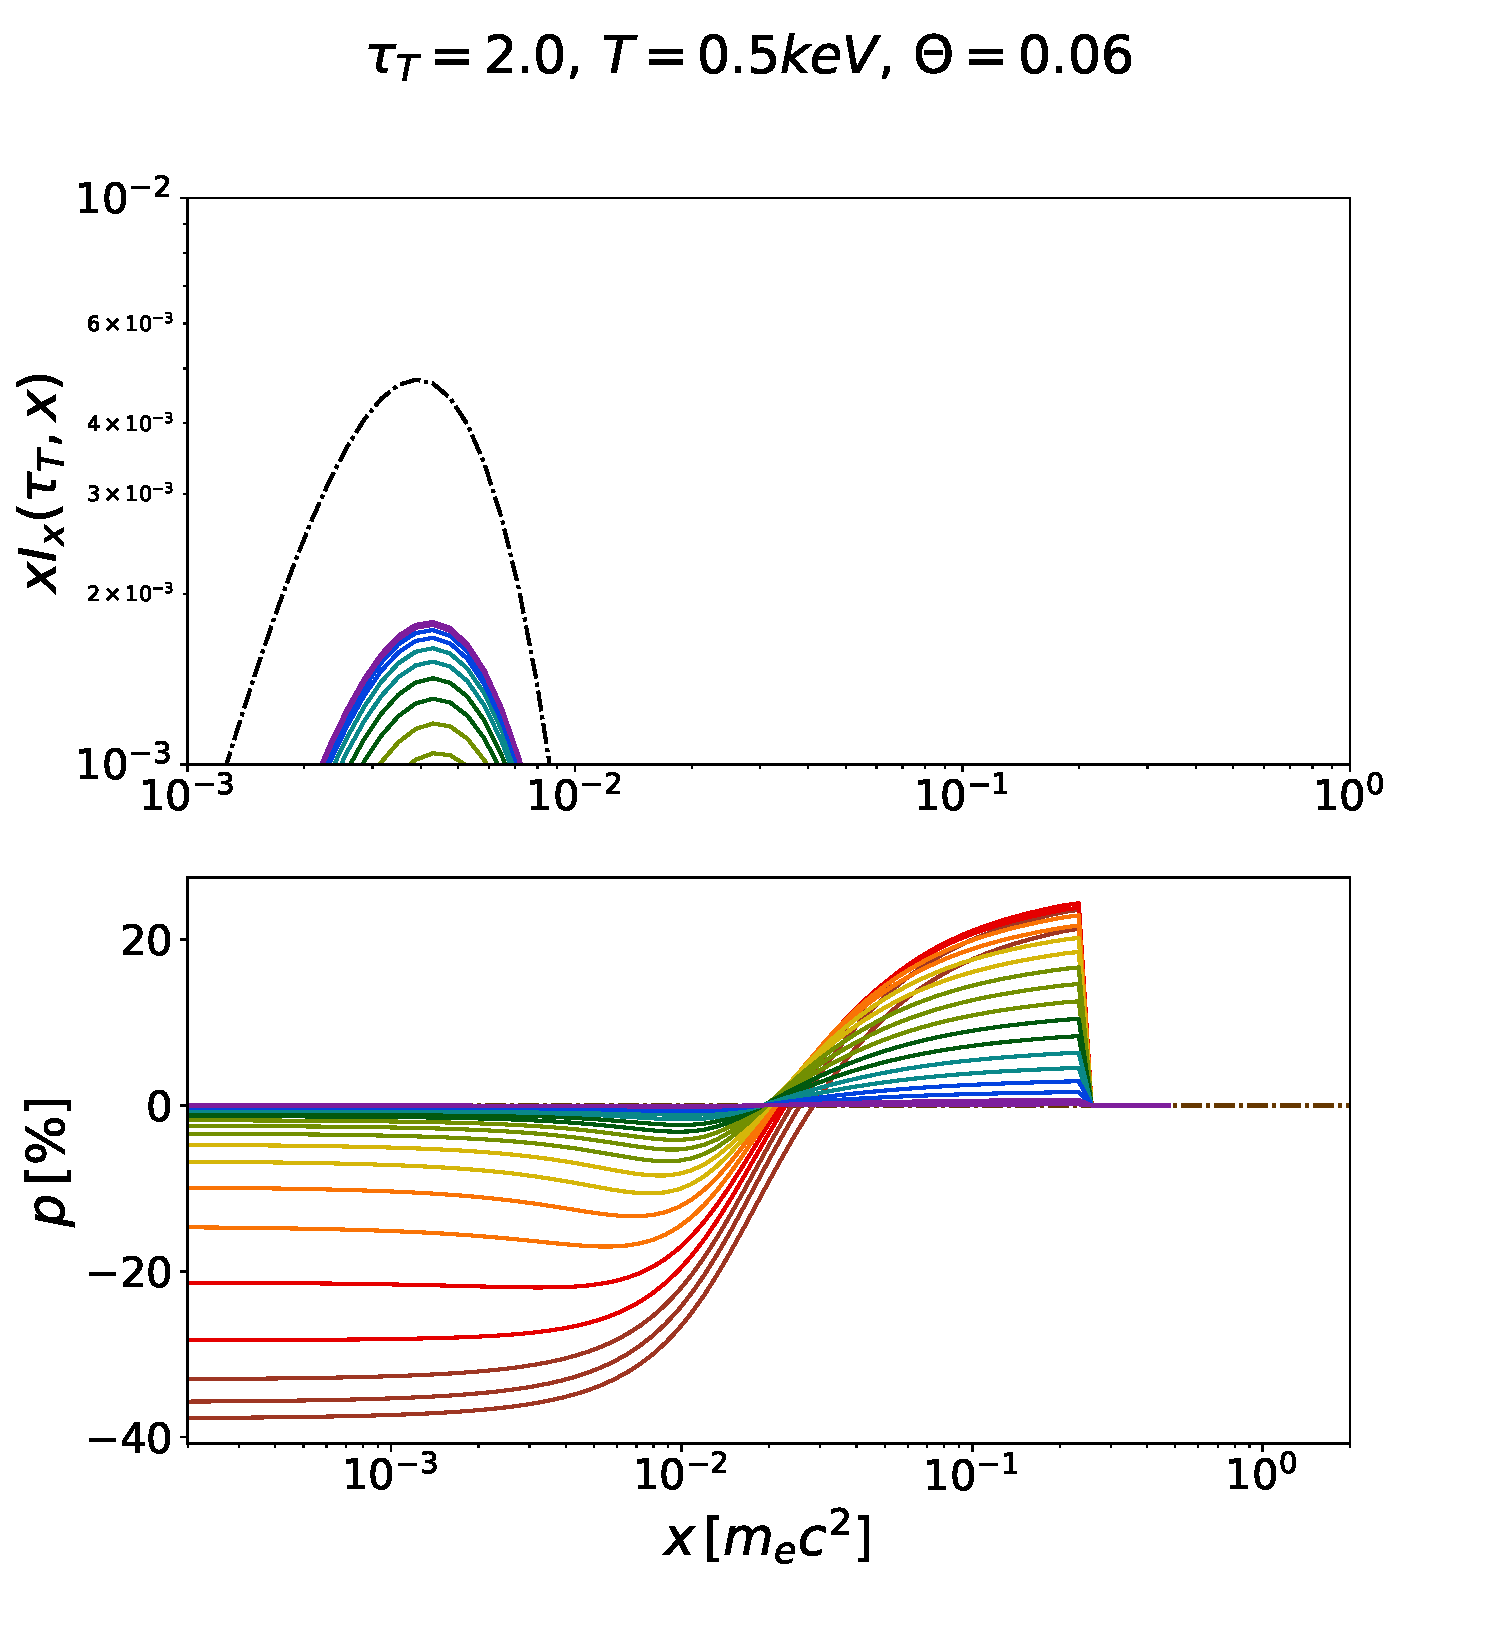
\includegraphics[width=\textwidth]{TM9zAll.pdf}
					\caption{\small\centering Поляризация в томсоновском приближении.}
				\end{subfigure}%
				\begin{subfigure}{.5\textwidth}
					\centering
					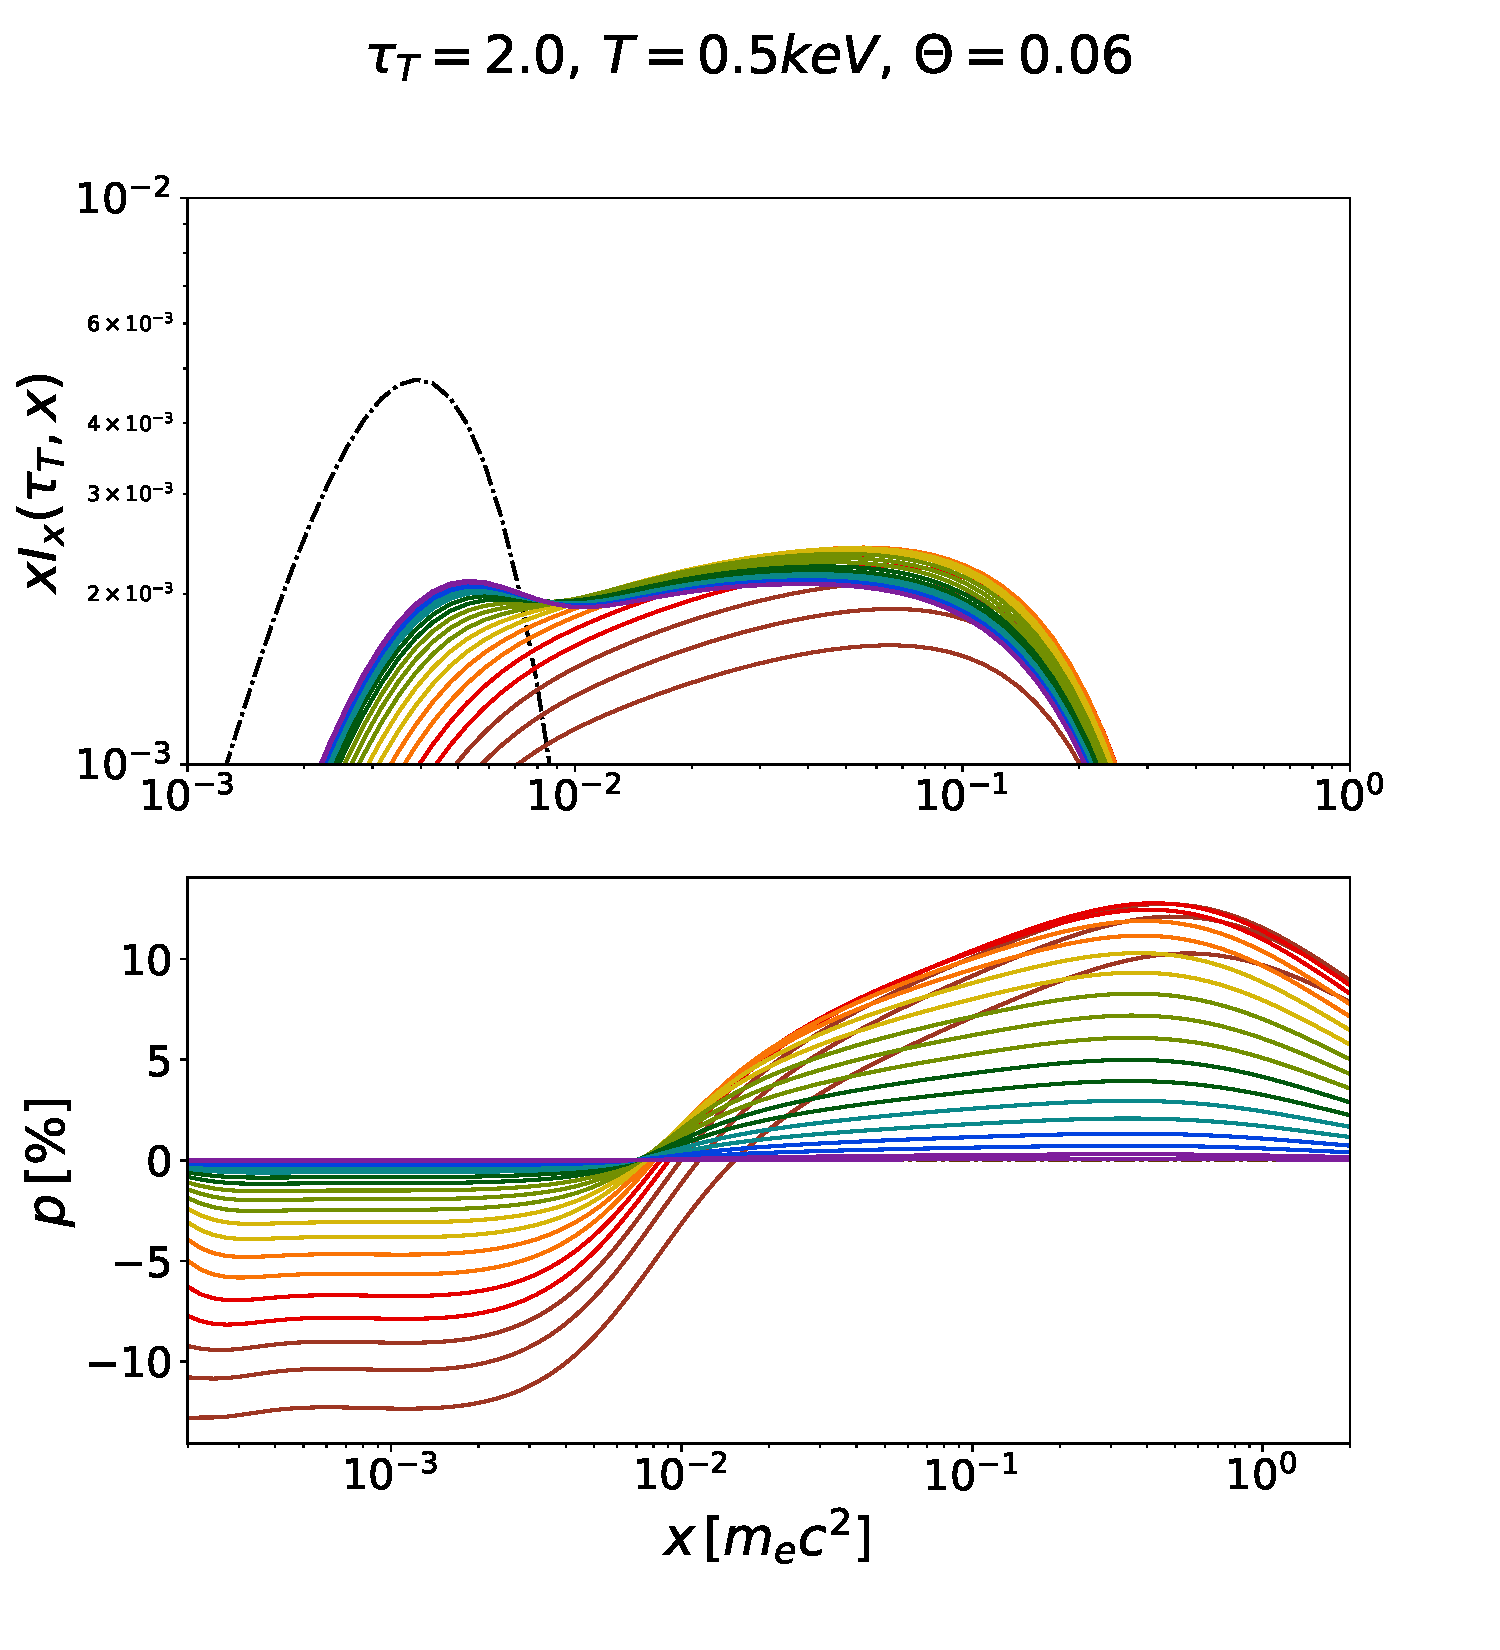
\includegraphics[width=\textwidth]{CM9zAll.pdf}
					\caption{\small\centering Комптоновское рассеяние.}\label{fig:Comp3}
				\end{subfigure}
				\caption{\small
					Сравнение Томсоновской и Комптоновской моделей. 
					Сравниваются исходящие с поверхности слоя плазмы фотоны под
					различными углами к вертикальному направлению. Например, черная линия на графике с рисунка \ref{fig:specificanglecomperison} здесь соответствуют одной из красных линий. Более синие цвета соответствуют более вертикальным направлениям излучения. 
					Для интегрирования по направлениям использовались гауссовы квадратуры, то есть линии соответствуют углам распространения, косинусы которых являются корнями полинома Лежандра, и, таким образом, сами углы соответствующие различным цветам являются почти равноотстоящими друг от друга. 
					Темно-коричневым штрих-пунктиром обозначен чернотельный спектр начальных фотонов на нижней границе слоя. 
					На верхних панелях изображены зависимости спектрального потока $xF_x$ в произвольных величинах от энергии.  
					На нижних панелях изображены соответствующие степени поляризации.
					}\label{fig:allcomparison}
			\end{figure}\newpage


		\subsection{Результирующие спектры}\label{sub:SI}

		На рисунках \ref{fig:C3C} и \ref{fig:C2C} приведены профили импульса и параметры поляризации для различных значений энергии, полученные для звезды с параметрами как на рисунке \ref{fig:allComp}. Рассматриваются различные конфигурации углов и спектры пятен. 

		% \textbf{\color{blue} What else... }
		\newpage
		\begin{figure}[H]
			\centering
			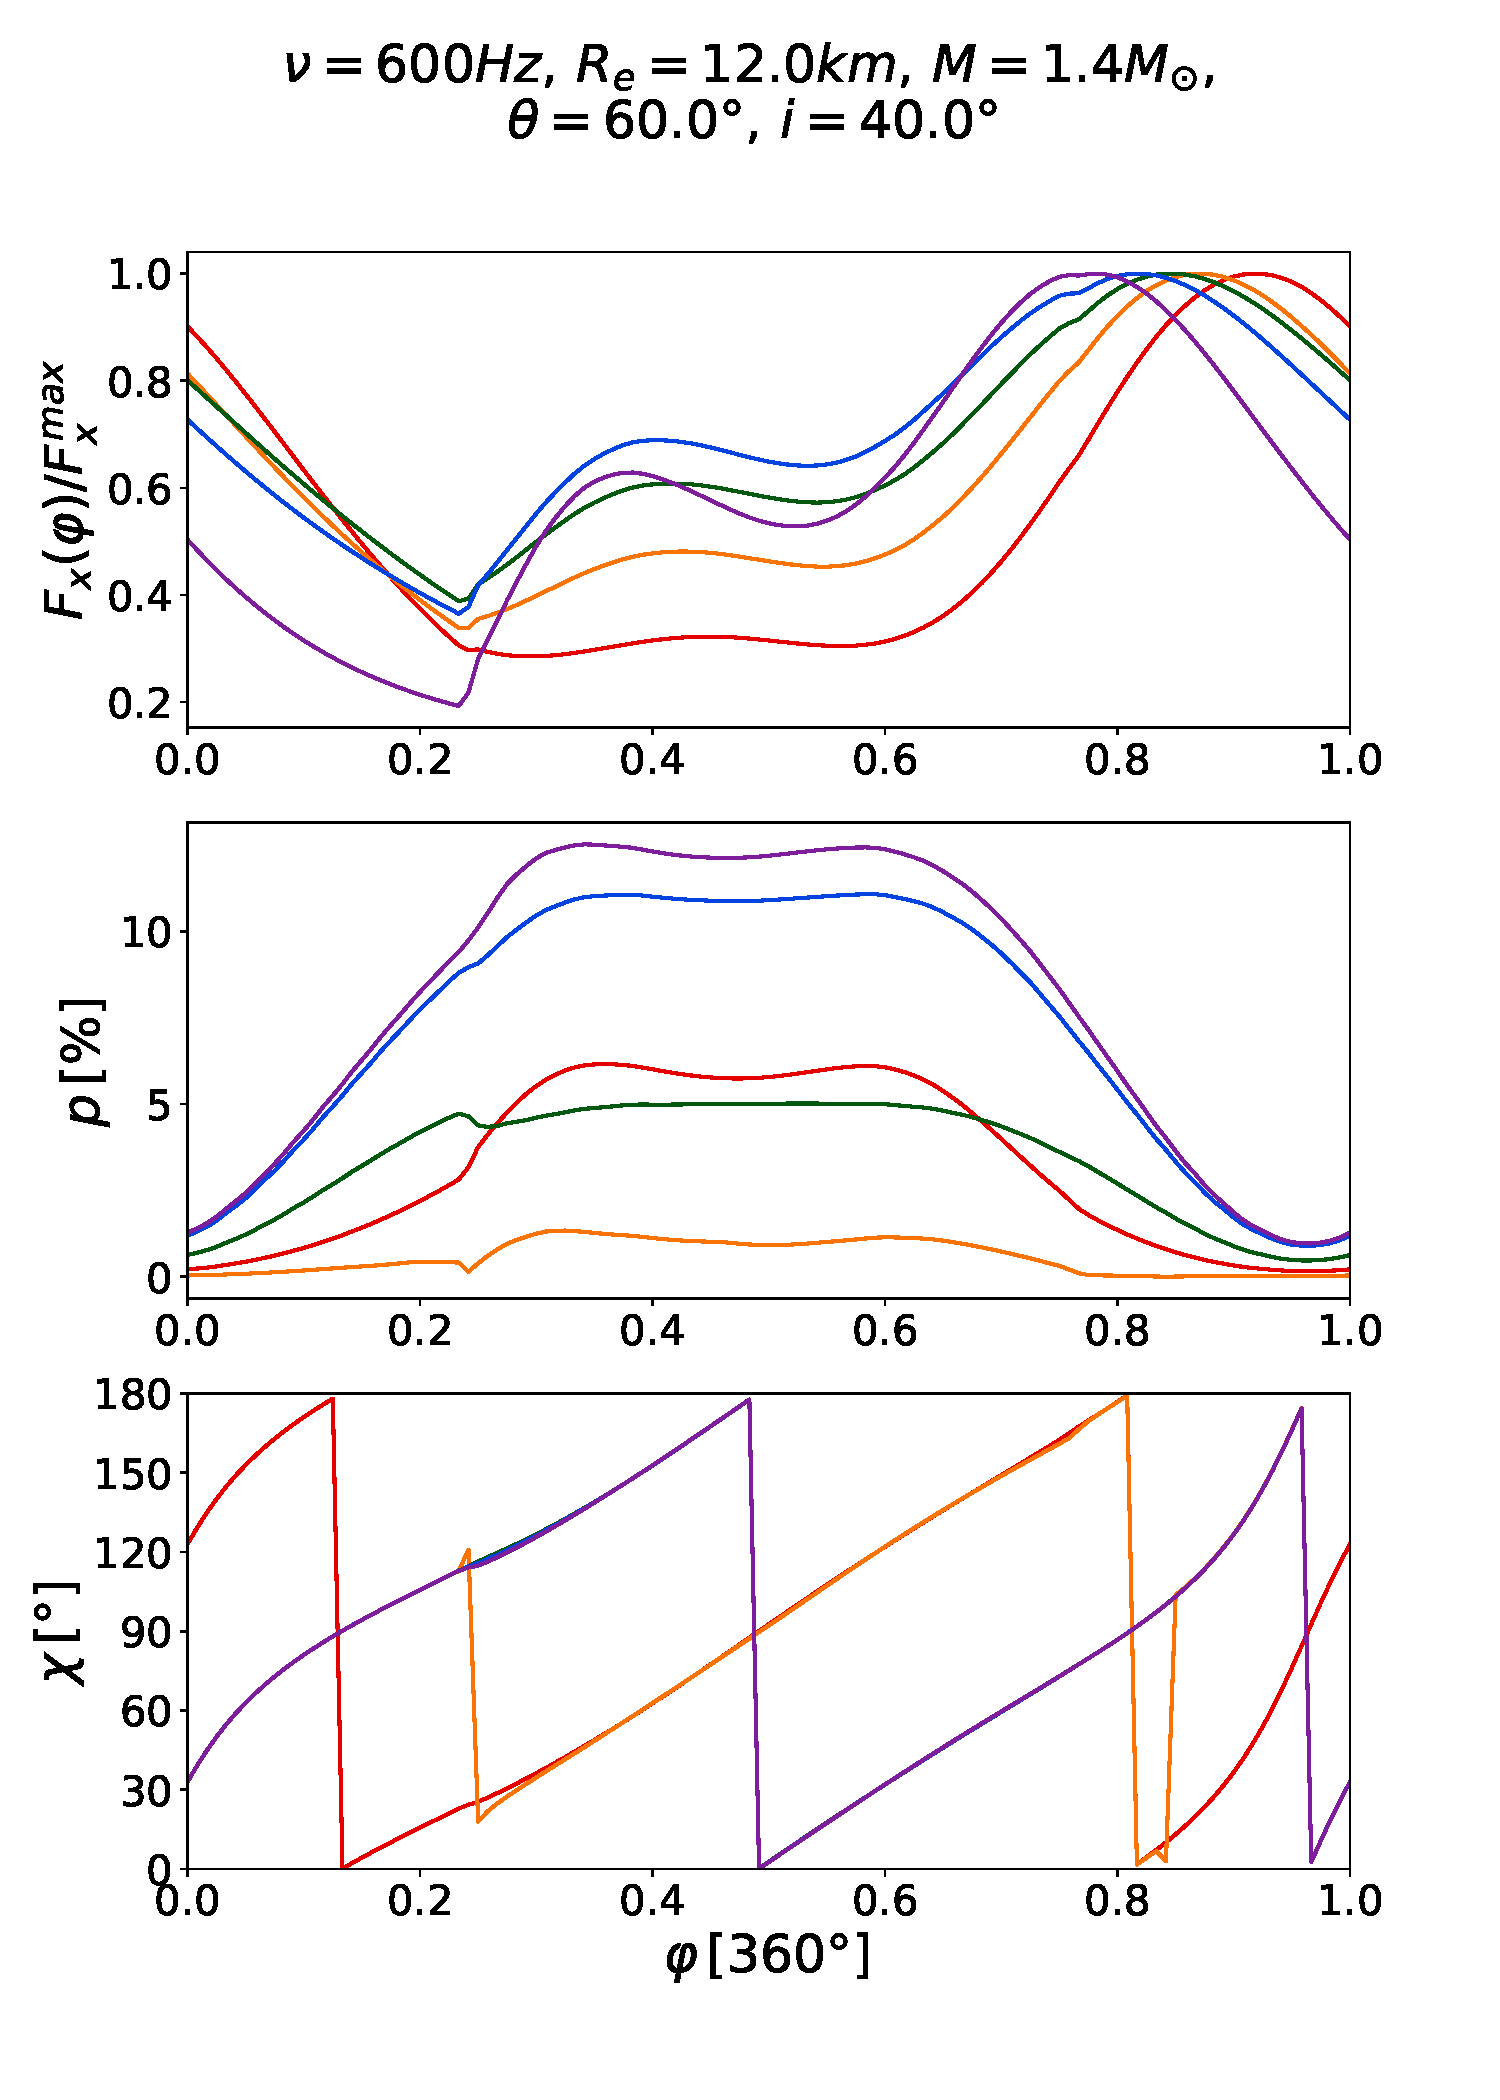
\includegraphics[width=0.8\textwidth]{CMComb12Ff.pdf}
			\caption{\small
				Профили импульса для пульсара с параметрами как на рисунке \ref{fig:allComp} с конфигурацией углов $\theta=60\degree,\,i=40\degree$.
				Спектр и поляризации исходящего от пятна излучения соответствуют рисунку \ref{fig:Comp3}.
				Цвета сопоставлены различным значениям энергии:
				красный --- 1 кэВ,
				оранжевый --- 3 кэВ,
				зеленый --- 7.5 кэВ,
				синий --- 58 кэВ,
				и фиолетовый --- 179 кэВ. На верхнем графике приведены потоки приходящего излучения, каждый кривая нормирована на свой максимум. 
				На среднем графике приведена степень поляризации, а на нижнем --- позиционный угол.
			}\label{fig:C3C}
		\end{figure}\newpage
		\begin{figure}[H]
			\centering
			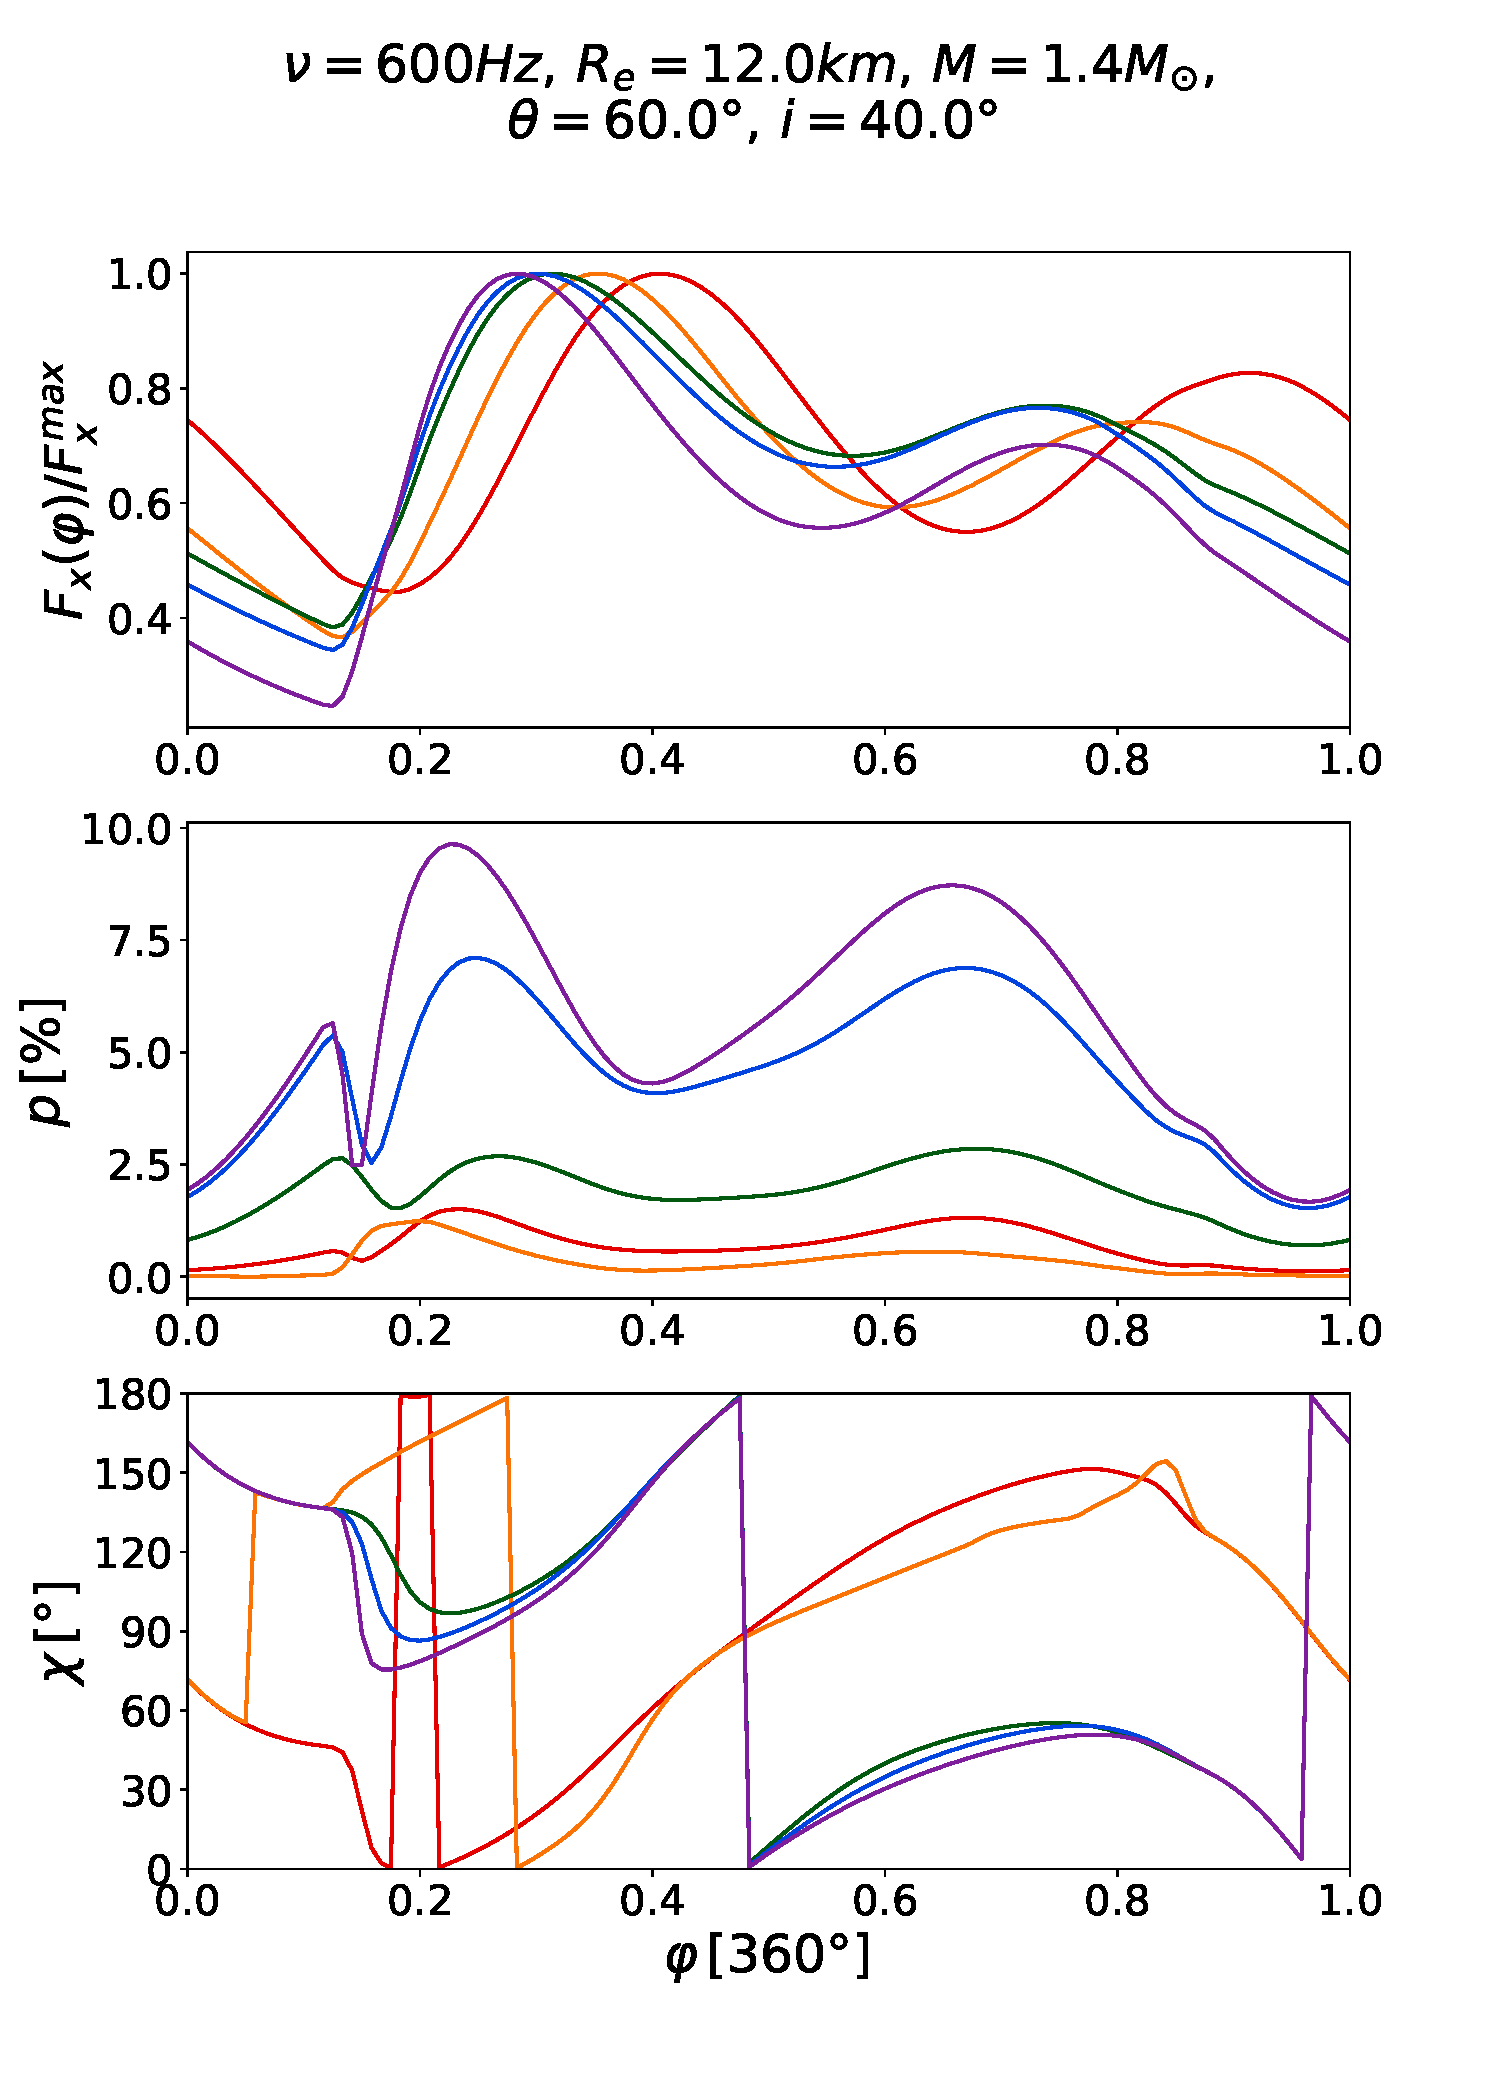
\includegraphics[width=0.8\textwidth]{CMComb11Ff.pdf}
			\caption{\small
				Графики профилей импульса аналогичные рисунку \ref{fig:C3C} но с конфигурацией углов $\theta=40\degree,\,i=60\degree$.
				Спектр и поляризации исходящего от пятна излучения соответствуют рисунку \ref{fig:Comp1}.
			}\label{fig:C2C}
		\end{figure}\newpage

		%C3Comb12Ff


	\newpage

	\section{Заключение}\label{conclusion}
		Был произведен учет и оценка эффектов связанных с несферичностью звезды.
		Эффекты сплюснутости для быстро вращающихся пульсаорв достигают нескольких процентов и могут значительно превышать вклад прочих эффектов которые обычно \cite{Poutanen2003,Viironen2004} учитываются при расчете профелей импульса. 
		Неучет этих эффектав может привести к пропорциональнм ошибкам при решении обратной задачи. 

		Было произведено сравнение поляризационных спектров полученных в приближении из статьи \cite{Viironen2004}  с реальными спектрами комптоновского рассеяния. 
		Зависимость степени поляризации от энергии для комптоновского и томсоновского рассеяний качественно получаются похожими друг на друга, однако систематически для комптонизованного спектра степень поляризации излучения ниже. 
		Для моделирования кривой интенсивности приближение томсоновского рассеяния использовать вообще нельзя, наклоны спектра получаются очень разными. 

		


		\newpage
	\bibliographystyle{unsrt}
	\bibliography{Thesis.bib}
	% \printbibliography
	\appendix
	% \textbf{\color{blue} Is any of that appendeces useful?}
		
	\newpage

		\section{Интегрирование по метрике Шварцшильда}\label{app:exact}
			Для численного расчета интеграла \eqref{eq:bendexact}, чтобы свести к интегрированию по конечному промежутку, нужно произвести замену переменных $y=R/r$
			\be
			\psi (R,\alpha) = \sin\alpha\int_0^1\df y {\left(1-u-y^2\sin^2\alpha(1-yu)\right)^{-\frac12}},
			\ee
			а после этого для раскрытия неопределенности на правом конце промежутка при $\sin \alpha \sim 1$ произвести вторую замену переменных $x=\sqrt{1-y}$
			\be\label{eq:2ndsub}
			\psi (R,\alpha) = \frac{2\sin\alpha}{\sqrt{1-u}}\int_0^1\frac{x\df x}{\sqrt{\cos^2\alpha+a\sin^2\alpha}},
			\ee
			где  
			\be
				a=x^2\left(2-x^2-\frac{u}{1-u}\left(1-x^2\right)^2\right).
			\ee
			Таким образом при $\cos\alpha\sim 0$ и $x \sim 0$ подынтегральное выражение в \eqref{eq:2ndsub} стремится к конечному значению \be
				\sqrt{\frac{1-u}{2-3u}}.
			\ee
			При $3u>2$ вокруг нейтронной звезды будут возможны замкнутые световые траектории. В данной работе эта возможность не рассматривается.
			Такие же замены переменных нужно произвести и для расчета интеграла \eqref{eq:timelag}.
	
	\newpage
		\section{Матрица перераспределения} \label{redistr}

			Матрица перераспределения $\bm{R}(x,\mu,x_1,\mu_1)$
			в уравнении \eqref{eq:Source}
			описывает вероятность для фотона, который до рассеяний имел энергию $x_1$ и направление распространения, определяющееся косинусом угла к вертикальному направлению $\mu_1$, после рассеяния на электроне иметь, соответственно, энергию $x$  и направление $\mu$.  
			Здесь и далее, индексом 1 маркированы величины, относящиеся к фотону до столкновения с электроном, а величины без индекса относятся к фотону после рассеяния.
			Для удобств	а интегрирования и представления результатов используется логарифмическая шкала безразмерных энергий 
			\be
			y=\ln x \qquad {y_1}=\ln x_1.
			\ee
			В таком случае становится удобным немного другое представление для матрицы перераспределения  
			\be
			\bm{R}^l(y,\mu,y_1,\mu_1)=\frac{x^2}{x_1}\bm{R}(x,\mu,x_1,\mu_1), \ee
			отличающееся от стоящего в уравнении \eqref{eq:Source} на множитель $x^2/x_1$, и тогда само уравнение примет немного упрощенный вид 
			\be
			S(\tau,y,\mu)= \int_{-\infty}^\infty \df y \int_{-1}^1 \df \mu_1 
			\bm{R}^l(y,\mu,y_1,\mu_1)\bm{I}(\tau,y_1,\mu_1).
			\ee
			Пределы интегрирования, естественно, не обязательно должны быть бесконечными, достаточно чтобы они содержали
			подавляющую долю всей энергии, иначе говоря, для вычислительных целей нижняя границы берется несколько ниже  $\log\frac{kT}{m_ec^2}$, а верхняя, выше $\log\Theta$.

			Формулы для вычисления матрицы $R$ представлены в работе \cite{Nagirner1993}.

			\be
			\bm{R}(x,\mu,x_1,\mu_1)=\int_0^{2\pi}\df \varphi 
			\bm{L}(-\chi)
			\bm{R}^t(x,x_1,\xi)
			\bm{L}(\chi_1),
			\ee


			$$
			\eta=\sqrt{1-\mu^2}, \qquad \eta_1=\sqrt{1-\mu_1^2},
			$$
			\be
			\xi=\cos\theta=\mu \mu_1 + \eta \eta_1 \cos \phi,
			\ee

			\be
			\bm{L}(\chi)=
			\left[{\begin{array}{cccc}
			    1 & 0 & 0 & 0 \\
			    0 & \cos{2\chi} & \sin{2\chi} & 0 \\
			    0 & -\sin{2\chi} & \cos{2\chi} & 0 \\
			    0 & 0 & 0 & 1  
			   \end{array} } \right],
			\ee

			\be\label{eq:coschi}
			\cos\chi=\frac{\mu_1-\mu\xi}{\eta\sin\theta},
			\qquad
			\cos\chi_1=\frac{\mu-\mu_1\xi}{\eta_1\sin\theta},
			\ee

			\be
			\label{eq:sinchi}
			\sin\chi=\frac{\eta_1\sin\varphi}{\sin\theta},
			\qquad
			\sin\chi_1=-\frac{\eta\sin\varphi}{\sin\theta}.
			\ee

			Из \eqref{eq:coschi} и \eqref{eq:sinchi} мы получаем значение тригонометрических функций для удвоенного угла $\chi$ 
			\be
			\cos2\chi=2\frac{(\mu_1-\mu\xi)^2}{\eta^2(1-\xi^2)}-1,
			\ee
			\be
			\cos2\chi_1=2\frac{(\mu-\mu_1\xi)^2}{\eta_1^2(1-\xi^2)}-1,
			\ee
			\be
			\sin2\chi\sin2\chi_1=-
			4\frac{(\mu_1-\mu\xi)(\mu-\mu_1\xi)\sin^2\varphi}{(1-\xi^2)^2}.
			\ee

			Из произведения трех матриц нужны только элементы левой верхней подматрицы 2 на 2 
			
			\be
			\bm{R}=
			\left[ {\begin{array}{cc}
			    R_{11} & R_{12}  \\
			    R_{21} & R_{22}  
			    \end{array} } \right]
			\ee
			
			которые равны $$
			R_{11}=\int_0^{2\pi} \df \varphi R^t ,
			$$$$
			R_{12}=\int_0^{2\pi} \df \varphi R^t_I\cos2\chi_1 ,
			$$$$
			R_{21}=\int_0^{2\pi} \df \varphi R^t_I\cos2\chi ,
			$$$$
			R_{22}=\int_0^{2\pi} \df \varphi (R^t_Q\cos2\chi\cos2\chi_1 + R^t_U \sin2\chi\sin2\chi_1),
			$$
			% The functions $R^t,\,R^t_I,\,R^t_Q,\,R^t_U$ are components of thermal Compton redistribution matrix $\bm{R}^t(x,x_1,\xi)$ 
			\be
			\bm{R}^t= 
			\left[ {\begin{array}{cccc}
			    R^t & R^t_I & 0 & 0 \\
			     R^t_I &  R^t_Q & 0 & 0 \\
			    0 & 0 &  R^t_U & 0 \\
			    0 & 0 & 0 &  R^t_V  
			   \end{array} } \right]
			\ee
			% which is obtained by taking an integral over electron Lorenz factor $\gamma$ with a distribution function $f(\gamma)$ which
			% in the case is given by the formula \eqref{eq:Maxwell}
			\be
			\bm{R}^t(x,x_1,\xi)=\frac38\int_{\gamma_*}^\infty \df \gamma
			f(\gamma)\bm{R}^m(x,x_1,\xi,\gamma)
			\ee

			$$
			q=xx_1(1-\xi),$$$$
			Q=\sqrt{(x-x_1)^2+2q},
			$$
			\be
			\gamma_*=\frac{x-x_1+Q\sqrt{1+2/q}}2,
			\ee

			% The matrix $\bm{R}^m$ is the Compton redistribution matrix for mono-energetic electron gas. If each electron has a Lorenz factor of $\gamma$ then the redistribution matrix in such gas is
			\be
			\bm{R}^m(x,x_1,\xi,\gamma)= 
			\left[ {\begin{array}{cccc}
			    R^m & R^m_I & 0 & 0 \\
			     R^m_I &  R^m_Q & 0 & 0 \\
			    0 & 0 &  R^m_U & 0 \\
			    0 & 0 & 0 &  R^m_V  
			   \end{array} } \right].
			\ee



			Матрица перераспределения имеет свойства симметричности относительно перестановки аргументов.

			Симметрия по энергиям:\be
			\bm{R}(x_1,\mu,x,\mu_1)=\bm{R}(x,\mu,x_1,\mu_1) e^\frac{x-x_1}\Theta. \ee
			Симметрия по направлениям:

			\be
			\bm{R}(x,\mu_1,x_1,\mu)=\bm{R}^T(x,\mu,x_1,\mu_1), \ee
			\be
			\bm{R}(x,-\mu,x_1,-\mu_1)=\bm{R}(x,\mu,x_1,\mu_1), \ee
			\be
			\bm{R}(x,-\mu_1,x_1,-\mu)=\bm{R}^T(x,\mu,x_1,\mu_1). \ee

\end{document}

